% !TeX spellcheck = de_DE

\newcommand{\tikzInfoVis}{
	\begin{tikzpicture}[
			align = center,
			repr/.style = {
				draw,
				rectangle,
				minimum width = 2cm,
				minimum height = 1cm,
			}
		]
		\node [repr] (rawData) {Rohdaten};
		\node [repr, right = 1.5 of rawData] (dataTables) {Daten-\\tabellen};
		\node [repr, right = 1.5 of dataTables] (visualStructures) {Visuelle\\Strukturen};
		\node [repr, right = 1.5 of visualStructures] (views) {View};
		\node [right = 1 of views] (human) {Mensch};
		\node [right = 1 of human] (task) {Aufgabe};

		\draw [->] (rawData) to node[below, yshift = -0.8cm](dataTransformation){Daten-\\transformation} (dataTables);
		\draw [->] (dataTables) to node[below, yshift = -0.8cm](visualMapping){Visuelle\\Abbildung} (visualStructures);
		\draw [->] (visualStructures) to node[below, yshift = -0.8cm](viewTransformation){View\\Transformation} (views);


		\path (dataTables.south) to coordinate(dataTablesNeedleA) (dataTables.south west);
		\coordinate [below left = 0.5 of dataTables, yshift = 0.15cm] (dataTablesNeedleB);
		\path (dataTables.west) to coordinate(dataTablesNeedleC) (dataTables.south west);

		\path (visualStructures.south) to coordinate(visualStructuresNeedleA) (visualStructures.south west);
		\coordinate [below left = 0.5 of visualStructures, yshift = 0.15cm] (visualStructuresNeedleB);
		\path (visualStructures.west) to coordinate(visualStructuresNeedleC) (visualStructures.south west);

		\path (views.south) to coordinate(viewsNeedleA) (views.south west);
		\coordinate [below left = 0.5 of views, yshift = 0.15cm] (viewsNeedleB);
		\path (views.west) to coordinate(viewsNeedleC) (views.south west);

		\draw [->] (dataTablesNeedleA) |- (dataTablesNeedleB) |- (dataTablesNeedleC);
		\draw [->] (visualStructuresNeedleA) |- (visualStructuresNeedleB) |- (visualStructuresNeedleC);
		\draw [->] (viewsNeedleA) |- (viewsNeedleB) |- (viewsNeedleC);

		\coordinate [below = 2.25 of human] (needle);

		\draw [->] (human) -- (needle) -| (dataTransformation);
		\draw [->] (human) -- (needle) -| (visualMapping);
		\draw [->] (human) -- (needle) -| (viewTransformation);

		\draw [dotted] (task) -- (human);
	\end{tikzpicture}
}

\newcommand{\tikzKdd}{
	\begin{tikzpicture}[
			align = center,
			repr/.style = {
				draw,
				rectangle,
				minimum width = 2.1cm,
				minimum height = 1cm,
			}
		]
		\node [repr] (data) {Daten};
		\node [repr, right = 1 of data, yshift = 1cm] (targetData) {Zieldaten};
		\node [repr, right = 1 of targetData, yshift = 1cm] (preprocessedData) {Vorverarb.\\Daten};
		\node [repr, right = 1 of preprocessedData, yshift = 1cm] (transformedData) {Transf.\\Daten};
		\node [repr, right = 1 of transformedData, yshift = 1cm] (patterns) {Muster};
		\node [repr, right = 1 of patterns, yshift = 1cm] (knowledge) {Wissen};

		\draw [->] (data) to coordinate(selection) node[yshift = 0.3cm, anchor = south east]{Selektion} (targetData);
		\draw [->] (targetData) to coordinate(preprocessing) node[yshift = 0.3cm, anchor = south east]{Vorverarbeitung} (preprocessedData);
		\draw [->] (preprocessedData) to coordinate(transformation) node[yshift = 0.3cm, anchor = south east]{Transformation} (transformedData);
		\draw [->] (transformedData) to coordinate(dataMining) node[yshift = 0.3cm, anchor = south east]{Data Mining} (patterns);
		\draw [->] (patterns) to coordinate(interpretation) node[yshift = 0.3cm, anchor = south east]{Interpretation\\und Evaluation} (knowledge);
		\coordinate [below = 0.75 of selection] (needle);
		\path let \p1 = (needle), \p2 = (interpretation) in coordinate(needle) at (\x2, \y1);
		\draw [->, dashed] (interpretation) -- (needle) -| (selection);
		\draw [->, dashed] (interpretation) -- (needle) -| (preprocessing);
		\draw [->, dashed] (interpretation) -- (needle) -| (transformation);
		\draw [->, dashed] (interpretation) -- (needle) -| (dataMining);
	\end{tikzpicture}
}

\NewEnviron{ivvaIntegration}{
	\begin{tikzpicture}[->, every node/.style = { draw, rectangle, minimum height = 0.75cm, minimum width = 2.5cm }]
		\node (daten) {Daten};
		\node [below = 0.5 of daten] (parameter) {Parameter};
		\node [below = 0.5 of parameter] (verfahren) {Verfahren};
		\node [below = 0.5 of verfahren] (zwErgebnis) {Zw.-Ergebnis};
		\node [below = 0.5 of zwErgebnis] (bewertung) {Bewertung};
		\node [below = 0.5 of bewertung] (ergebnis) {Ergebnis};
		\coordinate [above = 0.15 of verfahren.west] (a);
		\coordinate [below = 0.15 of verfahren.west] (b);
		\coordinate [left = 0.5 of a] (A);
		\coordinate [left = 0.5 of b] (B);
		\draw (verfahren) to (zwErgebnis);
		\draw (zwErgebnis) to (bewertung);
		\draw (bewertung) to (ergebnis);
		\draw (parameter) to (verfahren);
		\draw (daten) -| (A) -- (a);
		\draw [dashed] (bewertung) -| (B) -- (b);
		\BODY
	\end{tikzpicture}
}

\chapter{Einleitung}
	In dieser Zusammenfassung werden zwei Themen behandelt: Informationsvisualisierung und Visual Analytics. Dabei sollen die Frage beantwortet werden, wie verschiedene Daten \emph{gut} visualisiert werden können und wie Visualisierung die Analyse unterstützen können. Viele Ideen der folgenden Kapitel und grundlegender Techniken bauen dabei auf dem Verständnis grundlegender Prozesse des Gehirns ab. Denn: Eine Visualisierung soll dem Gehirn des*der Nutzer*in Arbeit abnehmen. Dabei sollen für jede Visualisierung die folgenden drei Fragen beantwortet werden:
	\begin{itemize}
		\item Was wird wie dargestellt?: Formale Beschreibung einer Visualisierung.
		\item Was ist gut und (möglichst) ohne Anstrengung sichtbar?: Prinzipien der Wahrnehmung kennen und anwenden.
		\item Was hilft dem*der Nutzer*in bei der Aufgabe?: Beschreibung und Wahrnehmungsprinzipien im Kontext einer Aufgabe bewerten.
	\end{itemize}
	Ein relevantes, bisher noch nicht erwähntes, Wort in den obigen Fragen ist die \emph{Aufgabe}. Zu Beginn jeder Visualisierung muss zunächst die \emph{Aufgabe} der Visualisierung identifiziert werden. Dies sind oftmals Entscheidungen, die (objektiv) durch Daten und Informationen getroffen werden (sollten). Dies ist in \autoref{fig:aufgabe} dargestellt. In der Praxis werden jedoch häufig einfach Visualisierungkataloge (große Datenbanken mit Visualisierungstechniken) nach einer "schönen" Visualisierung durchsucht. Dadurch wird das Dasein der Visualisierung als Werkzeug jedoch zu dem Zweck gemacht, \dh die Visualisierung wird ein Selbstzweck. Dies sollte eigentlich nie der Fall sein!

	Oft die Aussage getroffen, dass "ein Bild mehr sagt als tausend Worte." Im Allgemeinen sollte allerdings eher gesagt werden, dass ein Bild etwas \emph{anderes} als tausend Worte sagt: Sprachliche Artefakte (wozu auch Zahlen gehören), werden von dem Gehirn \emph{bewusst} und verarbeitet und oftmals in eine zeitliche Reihenfolge gebracht. Eine Visualisierung der selben Daten hingegen ist ein bildliches Artefakt und erlaubt eine \emph{unbewusste} Verarbeitung, bei der die Informationen im Raum strukturiert werden. Dadurch können komplexe Zusammenhänge sehr schnell vermittelt und erfasst werden.

	\begin{figure}
		\centering
		\begin{tikzpicture}[->, every node/.style = { draw, rectangle, minimum width = 3cm, minimum height = 0.75cm }]
			\node (daten) {Daten};
			\node [right = 1 of daten] (vis) {Visualisierung};
			\node [right = 1 of vis] (wissen) {Wissen};
			\node [right = 1 of wissen] (entscheidung) {Entscheidung};

			\draw (daten) -- (vis);
			\draw (vis) -- (wissen);
			\draw (wissen) -- (entscheidung);
		\end{tikzpicture}
		\caption[Von Daten zu Entscheidungen]{Eine Visualisierung dient immer der Erfüllung einer Aufgabe und soll zu einem Erkenntnisgewinn führen. Oftmals steht am Ende davon eine Entscheidung, die objektiv durch Daten getroffen werden soll. Bei der Erstellung einer Visualisierung sollte dieser Prozess also rückwärts durchgeführt werden, \dh ausgehend von der Frage, welche Entscheidung getroffen werden soll.}
		\label{fig:aufgabe}
	\end{figure}

	\section{Anwendungen von Visualisierungen}
		Die Anwendung einer Visualisierung, lässt sich in zwei Kategorien einteilen: \emph{Erfassen} und \emph{Produzieren} von Informationen, wobei erstere durch Informationsvisualisierung und letztere durch Visual Analytics "bearbeitet" werden.

		Innerhalb der Informationsvisualisierung werden die folgenden Gruppen unterschieden:
		\begin{itemize}
			\item \eqmakebox[ivAufgaben][l]{\emph{Explain:}} Es sollen bekannte Informationen an andere vermittelt werden (möglicherweise, aber nicht immer, interaktiv).
			\item \eqmakebox[ivAufgaben][l]{\emph{Explore:}} Es sollen neue Information auf Basis von Daten gefunden oder unsichere Informationen bestätigt werden (üblicherweise sehr interaktiv; das Ziel ist nicht immer bekannt).
			\item \eqmakebox[ivAufgaben][l]{\emph{Enjoy:}}   Zwanglose und durch Neugier getriebene Begegnung mit den Daten; dabei ist die Aufgabe selten bekannt.
		\end{itemize}
		Von diesen drei Arten der Informationsvisualisierung werden in dieser Zusammenfassung vor allem die ersten beiden behandelt.

		Innerhalb der Visual Analytics werden die folgenden Gruppen unterschieden:
		\begin{itemize}
			\item \eqmakebox[vaAufgaben][l]{\emph{Annotate}}
			\item \eqmakebox[vaAufgaben][l]{\emph{Record}}
			\item \eqmakebox[vaAufgaben][l]{\emph{Derive}}
		\end{itemize}
	% end

	\section{Identifizierung der Visualisierungsaufgabe}
		Bei der Identifizierung der Aufgabe sollte auch mit einbezogen werden,
		\begin{itemize}
			\item welche Informationen als bekannt vorausgesetzt werden,
			\item welche Informationen gesucht werden, und
			\item was mit den neuen Informationen gemacht wird oder gemacht werden soll.
		\end{itemize}
		Das Design der Visualisierung bestimmt damit essentiell, wie gut mit der Visualisierung gearbeitet werden kann durch Wiedererkennung bekannter Informationen und Erkennung neuer Informationen. Die erste Regel ist dabei, wie bereits erwähnt, das die Visualisierung ein Werkzeug und kein Selbstzweck ist. Das lässt sich wie folgt zusammenfassen:
		\begin{center}
			Have something to tell or something to ask!
		\end{center}
	% end

	\section{Negativbeispiele} % 1.47, 1.48, 1.49, 1.50, 1.51, 1.52, 1.53, 1.54, 1.55, 1.56, 1.57, 1.58, 1.59
		\todo{Content}
	% end
% end

\chapter{Der Informationsvisualisierungsprozess}
\label{c:visualisierungsprozess}

Der \emph{Informationsvisualisierungsprozess}, dargestellt in \autoref{fig:visualisierungsprozess}, wurde von Card et al. als Referenzmodell entworfen, um die Erstellung einer Visualisierung zu strukturieren. Dabei wird zwischen den Repräsentationen (\emph{Rohdaten}, \emph{Datentabellen}, \emph{Visuelle Strukturen} und \emph{Views}) unterschieden. Der Übergang zwischen den Strukturen wird durch die \emph{Datentransformation}, die \emph{Visuelle Abbildung} und die \emph{View Transformation} beschrieben. Eine weitere Zentrale Komponente ist der*die Nutzer*in (\emph{Mensch}), welche*r die einzelnen Schritte modifiziert. Dadurch wird das Modell zu einem Kreislauf der Visualisierung. In diesem Kapitel wird jeder Schritt separat behandelt, beginnend mit der Datentransformation (\autoref{sec:dataTransformation}) über die visuelle Abbildung (\autoref{sec:visualMapping}) bis zur Interaktion (\autoref{sec:interaktion}). Im folgenden wird eine kurze Übersicht über die Transformationsschritte gegebene:
\begin{itemize}
	\item \eqmakebox[infoVisProzess][l]{\emph{Datentransformation:}} Der der \emph{Datentransformation} werden die \emph{Rohdaten} in \emph{Datentabellen} umgewandelt. Diese können dann in den nächsten Schritten einfacher als die Rohdaten verarbeitet werden, da diese häufig ungeordnet und unstrukturiert vorliegen.
	\item \eqmakebox[infoVisProzess][l]{\emph{Visuelle Abbildung:}}  Bei der \emph{visuellen Abbildung} findet der Hauptteil der Visualisierung statt. Dabei werden einzelne Datenvariablen auf visuelle Attribute (\bspw die Position) abgebildet, was die \emph{visuellen Strukturen}.
	\item \eqmakebox[infoVisProzess][l]{\emph{Datentransformation:}} Abschließend werden in der \emph{View Transformationen} die tatsächlichen Datenwerte auf die Variablenwerte der visuellen Struktur abgebildet, woraus sich die tatsächliche Visualisierung, die \emph{View}, ergibt.
\end{itemize}
Die Unterscheidung zwischen der visuellen Abbildung und der View Transformation ist, dass ersteres beschreibt, \emph{dass} eine Datenvariable auf eine visuelle Variable abgebildet wird, und letzteres beschreibt, \emph{welcher} konkrete Datenpunkt auf welchen konkreten Wert abgebildet wird.

Der letzte Schritt im Informationsvisualisierungsprozess ist die Interaktion, welche durch die zurückgeführten Pfeile in \autoref{fig:visualisierungsprozess} dargestellt wird. Dies ist die technische Möglichkeit, die einzelnen Schritte zu verändern und anzupassen. Es soll dem*der Nutzer*in dabei möglich sein, einzelne Komponenten anzupassen, ohne auf eine neue Visualisierung des*der Designer*in zu warten. Für den*die Designer*in kann dadurch zu teilen das Problem gelöst werden, dass eventuell die genaue Aufgabe noch nicht bekannt ist.

\begin{figure}
	\centering
	\tikzInfoVis
	\caption[Informationsvisualisierungsprozess]{Der Informationsvisualisierungsprozess nach Card et al.}
	\label{fig:visualisierungsprozess}
\end{figure}

\section{Die Datentransformation}
	\label{sec:dataTransformation}

	Bei der Datentransformation werden die Rohdaten in Datentabellen umgewandelt, welche in den folgenden Schritten einfacher zu verarbeiten sind. Außerdem können eine Reihe an Vorverarbeitungstechniken (\bspw Datenbereinigung) angewandt werden. Dieser Abschnitt führt zunächst in die grundlegenden Datentypen und -strukturen sowie anschließend verschiedene Techniken der Vorverarbeitung ein.

	\subsection{Datentypen und Datenstrukturen}
		Zur Diskussion und Abbildung von Daten auf visuelle Strukturen ist es zunächst sinnvoll, die verschiedenen auftretenden Datentypen und -strukturen zu betrachten. Die Unterscheidung zwischen einem Typ und einer Struktur wird dabei grundlegend durch die Anzahl der zugeordneten Datenvariablen getroffen: Einfache Datentypen beziehen sich immer auf genau eine Datenvariable während Datenstrukturen Beziehungen zwischen mehreren Datenvariablen (welche meist Eigenschaften von Objekten, auch \emph{Items} genannt, sind) und Datensätzen beschreiben. Eine Visualisierung kann anschließend eine beliebige Kombination aus Datenvariablen, Items und Beziehungen abbilden.

		\subsubsection{Datentypen}
			Grundlegend wird zwischen \emph{nominalen}, \emph{ordinalen} und \emph{quantitativen} Datentypen unterschieden. Bei einem nominalen Datentyp ist dabei zwischen zwei Werten nur \emph{Gleichheit} und \emph{Ungleichheit} definiert. Dies können \zB Personen, Länder, etc. sein. Sind nur nominelle Daten zu visualisieren, kann eine Tabelle hier tatsächlich die beste Wahl sein! Ordinale Datentypen haben zusätzlich zu (Un-) Gleichheit noch eine \emph{Ordnung}, \bspw Schulnoten oder Rangordnungen. Der in Anzahl Operationen "mächtigste" Datentyp sind quantitative Daten, die auch noch \emph{Differenzen} und \emph{Differenzverhältnisse} haben. Ferner wird bei quantitativen Daten zwischen \emph{diskreten} und \emph{kontinuierlichen} Daten. Außerdem gibt es \emph{Intervall-} und \emph{Verhältnisskalen}: Auf ersterer sind Verhältnisse nicht vernünftig berechenbar, da die Skala keinen natürlichen Nullpunkt hat (\bspw Temperatur in \si{\degreeCelsius}). Letztere hat einen natürlichen Nullpunkt, weshalb auch Verhältnisse auf Werten Sinn ergeben (\bspw Temperatur in Kelvin). Des weiteren gibt es \emph{lineare} und \emph{zyklische} Skalen, bei der die Ordnung eine Totalordnung, \bzw eine "künstliche" Ordnung, ist.

			Die unterschiedlichen Datentypen sind in \autoref{fig:datentypen} zusammengefasst. Im Allgemeinen lässt sich also sagen, dass sich Datentypen vor allem durch die auf ihnen ausführbaren Operatoren unterscheiden. Außerdem ist nicht die Repräsentation, sondern die Bedeutung des Datentyps relevant (\bspw sehen Schulnoten aus wie Zahlen, sind aber ordinale Daten).

			\begin{figure}
				\centering
				\begin{tikzpicture}[align = center, class/.style = { }]
					\node [class] (datentypen) {\textbf{Datentypen}};

					\node [class, below = 1.5 of datentypen, xshift = -5cm] (nominal) {\textbf{Nominal}};
					\coordinate [below = 0.5 of nominal] (a);
					\node [right = 0.5 of a] (aa) {\eqmakebox[datentypenNominal][l]{(Un-) Gleichheit}};
					\draw (nominal) |- (aa);

					\node [class, below = 1.5 of datentypen] (ordinal) {\textbf{Ordinal}};
					\coordinate [below = 0.5 of ordinal] (b);
					\node [right = 0.5 of b] (ba) {\eqmakebox[datentypenOrdinal][l]{(Un-) Gleichheit}};
					\node [below = 0 of ba] (bb) {\eqmakebox[datentypenOrdinal][l]{Ordnung}};
					\draw (ordinal) |- (ba);
					\draw (ordinal) |- (bb);

					\node [class, below = 1.5 of datentypen, xshift = 5cm] (quantitativ) {\textbf{Quantitativ}};
					\coordinate [below = 0.5 of quantitativ] (c);
					\node [right = 0.5 of c] (ca) {\eqmakebox[datentypenQuantitativ][l]{(Un-) Gleichheit}};
					\node [below = 0 of ca] (cb) {\eqmakebox[datentypenQuantitativ][l]{Ordnung}};
					\node [below = 0 of cb] (cc) {\eqmakebox[datentypenQuantitativ][l]{Differenzen}};
					\node [below = 0 of cc] (cd) {\eqmakebox[datentypenQuantitativ][l]{Differenzverhältnisse}};
					\node [below = 0 of cd] (ce) {\eqmakebox[datentypenQuantitativ][l]{Diskret/Kontinuierlich}};
					\node [below = 0 of ce] (cf) {\eqmakebox[datentypenQuantitativ][l]{Intervall-/Verhältnisskala}};
					\node [below = 0 of cf] (cg) {\eqmakebox[datentypenQuantitativ][l]{Linear/Zyklisch}};
					\draw (quantitativ) |- (ca);
					\draw (quantitativ) |- (cb);
					\draw (quantitativ) |- (cc);
					\draw (quantitativ) |- (cd);
					\draw (quantitativ) |- (ce);
					\draw (quantitativ) |- (cf);
					\draw (quantitativ) |- (cg);

					\path (datentypen) to coordinate(needle) (ordinal);
					\draw (datentypen) -- (needle) -| (nominal);
					\draw (datentypen) -- (ordinal);
					\draw (datentypen) -- (needle) -| (quantitativ);
				\end{tikzpicture}
				\caption{Unterschiedliche Datentypen}
				\label{fig:datentypen}
			\end{figure}
		% end

		\subsection{Bildunterschriften}
			\label{subsec:caption}

			Eine \emph{Bildunterschrift} sollte immer eine kurze Interpretation/Einordnung des Bildes mit Verweisen auf die Abbildung enthalten. Dabei sollten das Bild und die Unterschrift idealerweise auch ohne den Haupttext verständlich sein, da die Abbildungen häufig als erstes angeschaut werden. Im Haupttext sollte nachher auf die Abbildung verwiesen, diese aber nicht beschrieben werden (die Beschreibung gehört in die Bildunterschrift). Ebenfalls sollte die zentrale Aussage der Grafik im Text wiedergefunden werden.
		% end
	% end

	\subsection{Vorverarbeitung}
		Ein wichtiger Teil der Datentransformation stell die Datenvorverarbeitung dar\footnote{Nach einer Studie von CrowdFlower im Jahr 2016 entfällt \SI{80}{\percent} der Zeit bei der Erstellung einer Visualisierung auf die Datensuche und -vorverarbeitung und nur etwas \SI{20}{\percent} auf die eigentliche Visualisierung.}. Da reale Daten oft "unsauber" sind, müssen diese bereinigt werden, um dem "Garbage In, Garbage Out"-Prinzip zu entgehen. \emph{Unsauber} hat dabei viele Facetten, \zB unvollständige und fehlende Werte, Rauschen, Inkonsistenz, Ausreißer und unglaubwürdiger Werte, und viele mehr. Die Vorverarbeitung umfasst dabei alle notwendigen Transformationen, die nicht von dem*der Nutzer*in durchgeführt werden können oder sollen. Wie immer ist die genaue Abgrenzung jedoch Abhängig von der Aufgabe und dem*der Nutzer*in: Ist das Fehlen von Werten beispielsweise keine wertvolle Information für den*die Nutzer*in, so sollten diese in der Vorverarbeitung von dem*der Entwickler*in bereinigt werden. Ein anderes Beispiel sind Ausreißer oder unplausible Werte: Ist der*die Entwickler*in bei der Interpretation der Daten überfordert, sollte die Verarbeitung als Datentransformation interaktiv durch den*die Nutzer*in durchführbar sein. Der Einfachheit halber wird deshalb im folgenden immer von (Daten-) Vorverarbeitung gesprochen, wobei jeder Schritt auch als interaktive Transformation dargestellt werden könnte.

		Bei der Vorverarbeitung sind insbesondere Metadaten (\zB Attributnamen, Referenzpunkte von Messungen, Einheiten, wichtige Schlüsselwörter) hilfreich. Außerdem werden häufig statistische Methoden wie Ausreißererkennung, Clusteranalyse, Korrelationsanalyse sowie statistische Plots und Histogramme verwendet.

		\subsubsection{Fehlende Werte und Datenbereinigung}
			Um fehlende Werte in den Daten zu korrigieren gibt es einige grundlegende Verfahren:
			\begin{itemize}
				\item \eqmakebox[vorverarbeitungFehlende][l]{\emph{Ignorieren:}} Die fehlenden Werte werden ignoriert und es wird gehofft, dass dies in der Visualisierung nicht tiefgreifend durchschlägt.
				\item \eqmakebox[vorverarbeitungFehlende][l]{\emph{Manuell Einfügen:}} Unter Nutzung von Expert*innenwissen werden die Daten manuell ergänzt. Dies ist zwar präzise, aber sehr zeitaufwendig.
				\item \eqmakebox[vorverarbeitungFehlende][l]{\emph{Eliminieren der Zeile:}} Zeilen mit fehlenden Werten werden entfernt. Dies ist die häufigste Methode, jedoch fehlt bei vielen Datensätzen in jeder Zeile mindestens ein Wert.
				\item \eqmakebox[vorverarbeitungFehlende][l]{\emph{Globale Konstante:}} Anstelle der fehlenden Werte wird eine globale Konstante, \zB \(-1\), eingesetzt. Dies verändert allerdings die Datenverteilung, was Probleme bei statistischen Analysen hervorrufen kann.
				\item \eqmakebox[vorverarbeitungFehlende][l]{\emph{Mittelwert:}} Die Werte werden durch den Mittelwert ersetzt. Dies ist gut für eine globale Statistik, die individuellen Abweichungen können allerdings groß sein.
				\item \eqmakebox[vorverarbeitungFehlende][l]{\emph{Wert basierenden auf Ähnlichkeit:}} Ersetzung der Werte durch Annahme, welche anderen Zeilen "ähnlich" sind.
			\end{itemize}
			Die konkrete Wahl einer dieser Methoden hängt dabei -- wie üblich -- stark von dem vorliegenden Problem ab, \zB des Typs und der Semantik der Daten, der Menge der fehlenden Werte und der Expertise des*der Anwenders*Anwenderin. Im Allgemeinen sollte immer versucht werden, den Grund für das Fehlen zu ermitteln. Außerdem muss bei einem Ersetzen der fehlenden Werte gespeichert werden, dass es sich um Ersatzwerte handelt!

			Im falle von fehlerhaften Werten, die häufig durch Menschen selbst verursacht werden, können ähnliche Methoden eingesetzt werden, allerdings sind diese sehr viel schwer zu detektieren.
		% end

		\subsubsection{Ausreißer (-detektion)}
			\emph{Ausreißer} sind Datenpunkte, die außerhalb des normalen Wertebereichs einer Datenvariable liegen. \emph{Starke} Ausreißer sind solche, die für Expert*innen ungewöhnlich und interessant sind. Dabei ist es nicht immer einfach zu entscheiden, was ein interessanter -- aber plausibler -- Ausreißer und was ein Fehler ist. Zur Detektion von Ausreißern werden deshalb häufig statistische Verfahren herangezogen. Eine einfache Methode ist die Annahme einer Normalverteilung und Ausschluss aller Werte, die um mehr als zwei Standardabweichungen vom Mittelwert abweichen. Das offensichtliche Problem dieser Annahme ist, dass sie häufig nicht gilt (\bspw da die Daten von mehreren Normalverteilungen stammen; dies kann durch Clustering detektiert werden, was später behandelt wird \todo{ref clustering}). Allerdings können, wie bereits erwähnt, Ausreißer auch plausibel und somit keine Datenfehler sein (ein Beispiel hierfür ist die Temperatur auf der Zugspitze, die plausibel einen Ausreißer im Vergleich zu meeresspiegelnahen Messstation darstellt).
		% end

		\subsubsection{Normalisierung und Skalierung}
			Oftmals würde ein einfaches Anzeigen der Daten dazu führen, dass viele der Datenpunkte an einem Ende der Skala "kleben." Hier kann eine Skalierung der Daten abhelfen, indem die Daten auf irgendeine Weise gestreckt/gestaucht werden. Dabei werden die Daten auf ein "normales" Intervall, \zB \([0, 1]\) oder \([-1, 1]\), abgebildet. Gängige Methoden sind:
			\begin{itemize}
				\item Min-Max-Normalisierung
					\begin{itemize}
						\item Linear
						\item Logarithmisch
						\item Wurzel
						\item Quadratisch
						\item Exponentiell
					\end{itemize}
				\item Weitere datenspezifische Normalisierungen (\bspw nach der Objektform)
				\item z-Score
				\item Quantil-Normalisierung
			\end{itemize}
			Bei der Min-Max-Normalisierung wird das Minimum \(\ell\) und das Maximum \(u\) der Daten verwendet, um die restlichen Daten zu skalieren. Zur Abbildung auf das Intervall \( [0, 1] \) gibt es \zB die folgenden Methoden\footnote{Zur Interpretation der logarithmischen Normalisierung kann es hilfreich sein, diese etwas umzuformen: \( (\log x - \log \ell) / (\log u - \log \ell) = \log(x/\ell) / \log(u/\ell) = \log_{u/\ell}(x/\ell) = \log_{u/\ell} x + \const_x \)}:
			\begin{align}
				f_\text{Linear}(x) & = \frac{x - \ell}{u - \ell}                     &
				f_\text{Log}(x)    & = \frac{\log x - \log \ell}{\log u - \log \ell} &
				f_\text{Quad}(x)   & = \bigl( f_\text{Linear}(x) \bigr)^2            &
				f_\text{Wurzel}    & = \sqrt{f_\text{Linear}(x)}
			\end{align}
			Für eine Normalisierung in den Bereich \( [-1, 1] \), was für negative, "bipolare", Werte sinnvoll ist, kann \zB wieder eine Min-Max-Normalisierung
			\begin{align}
				\hat{f}_\text{Linear}(x) & = 2 f_\text{Linear})(x) - 1
			\end{align}
			eingesetzt werden. Dabei kann es hilfreich sein, \(\ell\) und \(u\) als die absoluten Minima und Maxima zu definieren, \dh
			\begin{align}
				\ell' & = -\max\{ \lvert \ell \rvert, u \} &
				u'    & = \max\{ \lvert \ell \rvert, u \},
			\end{align}
			um sicherzustellen, dass \( \hat{f}_\text{Linear}(0) = 0 \) gilt (dies kann sonst zu einer Verzerrung führen, \bspw bei Temperaturen).

			\paragraph{Lokale und Globale Skalierung}
				Gibt es mehrere Datensätze mit unterschiedlichen Minima/Maxima (\zB Temperaturverlauf in mehreren Städten), so muss entschieden werden, welche Minima/Maxima verwendet werden. Dabei wird zwischen \emph{lokaler} und \emph{globaler} Normalisierung unterschieden: Bei der lokalen Normalisierung werden die Minima/Maxima jeden Datensatz bestimmt und angewendet, bei der globalen Normalisierung wird das Minimum/Maximum über alle Datensätze hinweg verwendet.

				Dabei gilt, wie so oft, dass die konkrete Wahl auch von dem konkreten Problem abhängt. Während bei einer lokalen Normalisierung die Wertverläufe gut verglichen werden können (\dh wann unterschiedliche Reihen \zB ihr Maximum erreichen), so können dabei die Werte nicht mehr direkt verglichen werden. Komplementär dazu können die Werte bei einer globalen Normalisierung gut verglichen werden, bei großen Unterschieden ist ein Verlaufsvergleich jedoch sehr schwer.
			% end
		% end

		\subsubsection{Diskretisierung}
			Werden kontinuierliche Daten verarbeitet, so ist es häufig nötig, diese zu diskretisieren, \dh diskrete Teilmengen als Approximation zu finden. Der Hauptgrund dafür ist, dass ein digitales System nicht mit "echt"-kontinuierlichen Daten umgehen kann, da sie inhärent diskret sind. Die üblichste Diskretisierungsdimension ist dabei die Zeit, bei der ein beliebiger Punkt \( t_k = k \Delta_t \) für einen Zeitindex \(k\) mit vorgeschriebener Schrittweite \(\Delta_t\) diskretisiert wird. Bei der Diskretisierung gehen allerdings Informationen verloren, was eventuell problematisch werden kann (vgl. Nyquist-Shannon-Abtasttheorem).
		% end

		\subsubsection{Sampling, Segmentierung und Untermengen}
			Um die Datenmenge zu reduzieren, gibt es verschiedene Ansätze. Eine davon ist \emph{Sampling}, wobei zufällige Stichproben aus den Daten gezogen werden, um die Datenpunkte in der Visualisierung zu reduzieren. Je nach Wahl der Verteilungsfunktion kann sich dadurch allerdings eine Verzerrung in den Daten und einiger statistischer Eigenschaften ergeben. Andere, nicht-zufalls-basierte, Methoden sind \emph{Segmentierung} und die Wahl von \emph{Untermengen}. Bei der Segmentierung werden die Daten in zusammenhängende Abschnitte/Regionen eingeteilt und einer Kategorie zugeordnet. Dies ist allerdings nicht immer eindeutig möglich. Die Wahl von Untermengen kann \bspw auf Basis von Filtern und anderen Einschränkungen erfolgen.
		% end

		\subsubsection{Datenintegration}
			Bei der \emph{Datenintegration} werden verschiedene Datenquellen zu einer einzigen Datenquelle vereint, was eventuell die Angleichung von Schemata und ähnlichem erfordert. Beispielsweise müssen bei der Integration imperialistischer und metrischer Quellen die Einheiten angepasst werden.
		% end
	% end
% end

\section{Die Visuelle Abbildung}
	\label{sec:visualMapping}

	In diesem Abschnitt wird die visuelle Abbildung, der dritte Schritt im Visualisierungsprozess (\autoref{fig:visualisierungsprozess}) genauer behandelt. Dabei ist die Abgrenzung zum vierten Schritt, der View Transformation, nicht immer scharf gezogen, da die Schritte eng zusammenhängen. In der Regel wird in der visuellen Abbildung eine Datenvariable auf eine visuelle Struktur abgebildet. Dies muss aber nicht immer exakt sein, \dh eine Variable kann auch auf mehrere Strukturen oder mehrere Variablen können auf die gleiche Struktur abgebildet werden (\bspw wird in einer Scatterplot-Matrix sowohl ein Datenwert als auch eine Dimension auf die Position abgebildet). Im Folgenden werden einige visuelle Strukturen ("Marks" und "Channels") eingeführt und ihre typische Anwendung beschrieben.

	Eine visuelle Abbildung muss immer die folgenden Dinge beinhalten: Titel, Skala und Achsenbeschriftungen (gegebenenfalls mit Einheit), Datenquelle, Legende und den Grafikkörper selbst. Außerdem sollte üblicherweise eine Bildunterschrift mit angegeben werden, siehe dazu \autoref{subsec:caption}.

	\subsection{Beispiele}
		\todo{Die Visuelle Abbildung: Beispiele; 2.3, 2.4, 2.5, 2.6; 2.7, 2.8, 2.9; 2.10, 2.11, 2.12}
	% end

	\subsection{Visuelle Strukturen}
		In diesem Abschnitt werden eine visuelle Strukturen -- auch \emph{Marks} und \emph{Channels} genannt -- eingeführt und ihre übliche Einsetzung beschrieben. Dabei beginnt jede Visualisierung grundlegend mit einem leeren Blatt, dem die visuellen Strukturen hinzugefügt werden.

		Der \emph{Raum}, \dh die Position auf der Abbildung, ist die bei weitem wichtigste und vielseitigste Struktur. Sofern nicht anders angegeben beziehen sich die Positionen immer auf zwei unabhängige\footnote{Die Wortwahl \emph{unabhängig} bezieht sich hier nur darauf, dass die Variablen selbst, nicht zwangsweise die Werte, unabhängig sind.} Variablen (\(x\) und \(y\)). Die Position ist dabei auch die einzige Struktur, die unabhängig von der Aufgabe und dem Datentyp verwendet werden kann und -- ebenfalls als einzige Struktur -- verwendet werden muss. Daher ist die Belegung der visuellen Raumvariablen die erste und wichtigste Designentscheidung. Innerhalb des Raumes werden anschließend weitere visuelle Strukturen platziert, die in Marks und Channels eingeteilt sind: \emph{Marks} sind geometrische Elemente, aus denen die Visualisierung zusammengesetzt sind, während \emph{Channels} Eigenschaften der Markierungen/Marks sind.

		Die visuelle Abbildungen besteht abschließend aus einer Zuordnung von Datenvariablen und Merkmalen auf Marks und Channels, siehe \autoref{fig:marksChannels}.

		\begin{figure}
			\centering
			\begin{tikzpicture}[->, blob/.style = { draw, rectangle, minimum height = 0.75cm, minimum width = 2cm }]
				\node [blob, label = above:Datenobjekt] (item) {Item};
				\node [blob, right = 4 of item, label = above:Merkmal] (value) {Wert};
				\node [blob, below = 2 of item, label = below:Visuelles Objekt] (mark) {Mark};
				\node [blob, right = 4 of mark, label = below:Visuelles Merkmal] (channel) {Channel};

				\draw (item) to node[above]{hat Merkmal} (value);
				\draw (item) to node[left]{Visuelle Abbildung} (mark);
				\draw (value) to node[right]{Visuelle Abbildung} (channel);
				\draw (mark) to node[below]{hat Merkmal} (channel);
			\end{tikzpicture}
			\caption{Beziehung zwischen Items, Werte, visuellen Channels und Marks}
			\label{fig:marksChannels}
		\end{figure}

		\subsubsection{Marks}
			\emph{Marks} sind die eigentlichen Strukturelemente, die auf der Visualisierung abgebildet werden, die häufig jeweils ein Item oder eine Relation repräsentieren. Die üblichsten sind dabei \emph{Punkte}, \emph{Linien}, \emph{Flächen} und \emph{Text} wobei letzterer nur sehr sparsam und am besten gar nicht eingesetzt werden sollte. Zur Auswahl eines Marks sollten mehrere Aspekte in Betracht gezogen werden, insbesondere die Daten, die repräsentiert werden sollen (einzelne Items, Item-Paare, Teilmengen von Items, ein Attribut, etc.). Zum Verständnis der Visualisierung kann es hilfreich sein, wenn eine eingängige Metapher zwischen den repräsentierten Daten und der Visualisierung besteht (\zB Darstellung eines Volumens durch eine Fläche). Dabei stellen Linien häufig dar, dass ein Änderung kontinuierlich verläuft, während Punktmengen und ähnliches andeuten, dass eine Änderung diskret ist. Des weiteren sollte bei der Auswahl der Marks darauf geachtet werden, dass die genutzten Marks die benötigten Channels (siehe nächster Abschnitt) unterstützen.

			Eine Ambiguität zwischen den obigen Marks ist die Unterscheidung zwischen einem Punkt und einer Fläche: Wann ist ein Punkt "so groß", dass er eigentlich eine Fläche ist? Dies kann dadurch aufgelöst werden, dass ein Punkt allgemein eine Markierung bezeichnet, die etwas 0-Dimensionales darstellt, \dh auch ein großer Punkt markiert ausschließlich einen Punkt, indem der Bezug zum Hintergrund verschieden ist.
		% end

		\subsubsection{Channels}
			\label{subsubsec:channels}

			\emph{Channels} sind die visuellen Eigenschaften von Marks, \dh diese können zusätzlich als Unterscheidungs- und Identifikationsmerkmal eingesetzt werden. Dabei unterscheiden sich die anwendbaren Channels nach den eingesetzten Marks. Eine Übersicht über die üblichsten Channels ist in \autoref{fig:channels} zu finden. In diesem Abschnitt werden diese üblichen Channels sowie einige nicht häufig anzutreffende Channels vorgestellt. Ebenfalls wird auf die Rolle der Elemente im Designprozess eingegangen, wobei der Grund für diese Rolle in \autoref{sec:wahrnehmung} behandelt wird. Eine Übersicht über die Eignung der gängigsten Channels für verschiedene Datentypen und Aufgaben ist in \autoref{tab:channelsDatentypen} \bzw \autoref{tab:channelsAufgaben} gegeben.

			Im allgemeinen sollten nicht zu viele Channels verwendet werden, da die Abbildung dadurch chaotisch wird. Im konkreten Fall hängt die genaue Anzahl natürlich immer von der Aufgabe ab. Für Explain- und Explore-Aufgaben sollten generell eher weniger Channels verwendet werden, damit die Visualisierung verständlich bleibt. Außerdem sollte bei "Explore" vermieden werden, dass dominante Channels die Wahrnehmung von Mustern in anderen Channels verhindern. Bei "Enjoy" hingegen ist absolute Freiheit gegeben.

			\begin{table}
				\centering
				\begin{tabular}{l|l|l}
					\toprule
					\textbf{Punkt} & \textbf{Linie}                       & \textbf{Flächen}                  \\ \midrule
					Position       & Position                             & Position                          \\
					Farbe          & Farbe                                & Farbe                             \\
					Helligkeit     & Helligkeit                           & Helligkeit                        \\
					Form           & Breite                               & Kanteneigenschaften (siehe Linie) \\
					Orientierung   & Stil (Gestrichelt, Gepunktet, \dots) & Tiefe                             \\
					Größe          & Größe/Länge                          & Größe/Fläche                      \\
					Textur         & Dynamik                              & Textur                            \\ \bottomrule
				\end{tabular}
				\caption{Übliche Channels}
				\label{fig:channels}
			\end{table}

			\begin{table}
				\centering
				\begin{tabular}{c|ccccc}
					\toprule
					                       & \textbf{Nominal} & \textbf{Ordinal} & \textbf{Quantitativ} & \textbf{Räumlich} & \textbf{Zeitlich} \\ \midrule
					\textbf{Position}      & \(+\)            & \(+\)            & \(+\)                & \(+\)             & \(+\)             \\
					\textbf{Länge}         & \(-\)            & \(+\)            & \(+\)                & \(?\)             & \(?\)             \\
					\textbf{Größe}         & \(-\)            & \(+\)            & \(\circ\)            & \(-\)             & \(-\)             \\
					\textbf{Farbsättigung} & \(-\)            & \(+\)            & \(\circ\)            & \(-\)             & \(-\)             \\
					\textbf{Textur}        & \(+\)            & \(+\)            & \(-\)                & \(-\)             & \(-\)             \\
					\textbf{Farbton}       & \(+\)            & \((-)\)          & \(-\)                & \(-\)             & \(-\)             \\
					\textbf{Orientierung}  & \(+\)            & \(+\)            & \(-\)                & \(-\)             & \(-\)             \\
					\textbf{Form}          & \(+\)            & \(-\)            & \(-\)                & \(-\)             & \(-\)             \\ \bottomrule
				\end{tabular}
				\caption{Übliche Channels und deren Eignung für verschiedene Datentypen}
				\label{tab:channelsDatentypen}
			\end{table}
			\begin{table}
				\centering
				\begin{tabular}{c|ccccc}
					\toprule
					                       & \textbf{Grupp.} & \textbf{Sel./Hervorhebung} & \textbf{Vgl. Anord.} & \textbf{Vgl. Quant.} & \textbf{Unterscheidbarer Werte} \\ \midrule
					\textbf{Position}      & \(+\)           & \(+\)                      & \(+\)                & \(+\)                & Bildschirmgröße                 \\
					\textbf{Länge}         & \(-\)           & \((+)\)                    & \(+\)                & \(+\)                & ca. \numrange{5}{15}            \\
					\textbf{Größe}         & \(-\)           & \(+\)                      & \(+\)                & \(+\)                & ca. \numrange{5}{15}            \\
					\textbf{Farbsättigung} & \(-\)           & \(+\)                      & \(+\)                & \(+\)                & ca. \numrange{5}{7}             \\
					\textbf{Textur}        & \(+\)           & \(+\)                      & \(+/-\)              & \(+/-\)              & ca. \numrange{5}{7}             \\
					\textbf{Farbton}       & \(+\)           & \(+\)                      & \(-\)                & \(-\)                & ca. \numrange{7}{8}             \\
					\textbf{Orientierung}  & \(+\)           & \(+\)                      & \(\circ\)            & \(\circ\)            & ca. \numrange{4}{6}             \\
					\textbf{Form}          & \(+\)           & \(\circ\)                  & \(-\)                & \(-\)                & ca. \numrange{5}{7} "neutrale"  \\ \bottomrule
				\end{tabular}
				\caption[Übliche Channels und deren Eignung für verschiedene Aufgaben]{Übliche Channels und deren Eignung für verschiedene Aufgaben. Abkürzungen: "Grupp." ist "Gruppierung", "Sel." ist "Selektion", "Vgl." ist "Vergleich", "Anord." ist "Anordnung" und "Quant." ist "Quantitäten".}
				\label{tab:channelsAufgaben}
			\end{table}

			\paragraph{Farbkanäle (Farbton, Helligkeit, Sättigung)}
				Ein sehr häufiger Channel ist die Farbe von Marks, die gleich drei verschiedene Channels aufweist: Farbton, Helligkeit und Sättigung, wobei allerdings Helligkeit und Sättigung praktisch niemals zeitgleich genutzt werden. Die Farbe kann dabei viele verschiedene Werte diskreter und kontinuierlicher Natur darstellen und ist die einzige Struktur, die auch bei nur einem Pixel funktioniert. Die Nutzbarkeit und Barrierefreiheit ist jedoch stark von der gewählten Farbskala abhängig (dies wird in \autoref{subsec:farbe} genauer behandelt).
			% end

			\paragraph{Länge}
				Neben der Position ist die \emph{Länge} eines Objekts das einzige Attribut, welches numerische Größenverhältnisse exakt abbilden kann (im Falle von parallelen Längen sogar besser als die Position). Jedoch ist die Wahrnehmung stark beeinflussbar, weshalb die Darstellung sehr einfach sein muss, wenn tatsächlich numerische Vergleiche durchgeführt werden sollen, \dh alles außer Länge und Position sollte weggelassen werden (Balkendiagramme).
			% end

			\paragraph{Größe und Flächeninhalt}
				Für einen qualitativen Vergleich ist es naheliegend, Größenordnungen zu vergleichen. Insbesondere bei einer Fläche sind \emph{Differenzen} allerdings sehr schwer vergleichbar, da die Fläche quadratisch mit der Breite skaliert. Des weiteren sind Länge und Breite nicht als separate Channels zu betrachten, da sich dadurch eine Fläche ergibt, deren Größe eher wahrgenommen wird. Dadurch können die eigentlichen Daten überdeckt werden. Ein weiterer Nachteil ist, dass die Größe als Platz benötigt.
			% end

			\paragraph{Form}
				Die \emph{Form} kann als Channel sehr gut gelernt werden, \dh die Formen erhalten über die Zeit eine feste Bedeutung für den*die Nutzer*in und sie werden wiedererkannt. Da es sehr viele vorstellbare Formen gibt, könnten an sich sehr viele Formen in einer Grafik verwendet werden, jedoch ist mit üblichen Formen bereits eine Bedeutung verknüpft, was verwirrend sein kann (\bspw ein Herz als Darstellung für etwas schlechtes oder Pfeile, die auf nichts zeigen). Daher werden in der Praxis häufig "neutrale" Formen wie Kreise, Quadrate, oder Dreiecke verwendet.
			% end

			\paragraph{Orientierung}
				Die \emph{Orientierung} eines Marks kann ebenfalls genutzt werden, um Daten darzustellen (\bspw die Orientierung eines Pfeils). Natürlich kann dies nur bei bestimmten Formen genutzt werden, abhängig von den Symmetrien der Form. Außerdem ist der Übergang von einer Form mit variabler Orientierung und zwei verschiedenen ähnlichen Formen nicht strikt.
			% end

			\paragraph{Exoten}
				Einige Exoten unter den Channels sind \bspw Tiefe/Überdeckung, Schatten (und die Richtung dessen), Textur, Animation/Bewegung, Schattierung und Unschärfe. Diese sollen allerdings nicht oder nur sehr sparsam eingesetzt werden!
			% end
		% end

		\subsubsection{Glyphen}
			\emph{Glyphen} sind eine spezielle Art von Marks, die insbesondere bei kartographischen Abbildungen (siehe \autoref{sec:karten}) verwendet werden. Ein Glyph kann dabei beliebig komplex sein und viele Channels und Marks kombinieren, sollten dabei aber intuitiv bleiben; sie stellen eine \emph{gemischte Visualisierung} dar. Bei Seekarten sind dies zum Beispiel die Markierungen der Tonnen auf den Seestraßen (siehe \autoref{fig:glyph}). Formal ist ein Glyph ein "kleines, unabhängiges, visuelles Objekt, welches Merkmale von einem oder mehreren Items zeigt". Dabei kann ein Glyph viele andere Zeichen und Visualisierungen umfassen. Da diese Definition sehr allgemein ist, muss bei dem Design von Glyphen immer zwischen Komplexität eines Glyphs und der zu erwartenden Anzahl Glyphen abgewägt werden. Dabei sollten die Glyphen einfacher sein, wenn Muster statt Werte relevant sind oder die Wertverteilung "chaotisch" sein könnte. Wie auch bei "großen" Visualisierungen ist es wichtig festzulegen, welche Datenattribute welche Channels nutzen (hier können alle bereits erwähnten und noch zu erwähnenden Richtlinien angewandt werden).

			Als noch weiter gefasste Variante eines Glyphs kann ein solches sogar selbst wieder Visualisierungen enthalten, \bspw Starplots innerhalb eines Scatterplots. Häufig genutzt werden außerdem Torten-, Linien- und Balkendiagramme. Dabei nutzen die Glyphen nur den Grafikkörper, Achsen und Achsenbeschriftungen werden bewusst ausgelassen, um die Darstellung zu komprimieren.

			\begin{figure}
				\centering
				\includegraphics[width=0.8\linewidth]{glyphen\IfDarkModeT{-dark}}
				\caption[Beispiel eines Glyphs auf Basis einer Seekarte]{Auf diesem Seekartenausschnitt ist zu sehen, wie die Tonnen Außenelbe-Reede 2 und 4 durch Glyphen dargestellt werden, die viele Informationen transportieren. Bei ersterer ist \bspw die Information enthalten, dass es sich um eine gelbe einfarbige Tonne ohne Toppzeichen mit unterbrochenem Feuer in dreier-Gruppen in Gelb und einer Wiederkehr von \SI{12}{\second} handelt.}
				\label{fig:glyph}
			\end{figure}
		% end
	% end

	\subsection{Bildunterschriften}
		Eine \emph{Bildunterschrift} sollte immer eine kurze Interpretation/Einordnung des Bildes mit Verweisen auf die Abbildung enthalten. Dabei sollten das Bild und die Unterschrift idealerweise auch ohne den Haupttext verständlich sein, da die Abbildungen häufig als erstes angeschaut werden. Im Haupttext sollte nachher auf die Abbildung verwiesen, diese aber nicht beschrieben werden (die Beschreibung gehört in die Bildunterschrift). Ebenfalls sollte die zentrale Aussage der Grafik im Text wiedergefunden werden.
	% end
% end

\section{Wahrnehmung, Position und Layout}
	\label{sec:wahrnehmung}

	In diesem Abschnitt werden die elementaren visuellen Aufgaben sowie die Wahrnehmung verschiedener Channels behandelt. Daraus werden abschließend Begründungen für oder gegen bestimmte Designentscheidungen abgeleitet.

	\subsection{Wahrnehmungsmodelle von Ware}
		\label{subsec:wahrnehmungWare}

		Das visuelle System des Menschen ist in mehrere Schichten geteilt (V1 bis V5), die unterschiedliche Aufgaben erfüllen, wobei die zu erfüllenden Aufgaben mit steigender Schicht komplexer und abstrakter werden. Die Schichten sind dabei in beide Richtungen verbunden und die Funktion und Interaktion zwischen den Schichten ist ein offenes Forschungsthema. Diese Idee der Schichten wurde von Colin Ware zu dem \emph{Wahrnehmungsmodell (von Ware)} zusammengefasst, welches die ablaufenden Prozesse in drei Gruppen/Stufen einteilt:
		\begin{enumerate}
			\item Parallele Verarbeitung elementarer visueller Merkmale statt. Diese Verarbeitung ist dabei nicht erlernbar und bei allen Menschen zum Großteil gleich.
			\item Mustererkennung; langsame und serielle Verarbeitung, welche trainierbar ist, sodass weniger Aufmerksamkeit benötigt wird.
			\item Sequentielle und zielgerichtete Verarbeitung; sehr langsame, aufmerksam gesteuerte, Übersetzung visueller Objekte in Sprache und anders herum.
		\end{enumerate}
		Die Kommunikation zwischen den Stufen verläuft dabei ebenfalls in beide Richtungen. Da die Wahrnehmung des gleichen Bildes nicht zu jedem Zeitpunkt und jedem Menschen das gleiche Ergebnis liefert, \dh die Verarbeitung ist nicht streng deterministisch, gibt es keine absolut "richtigen" und "falschen" Design für bestimmte Menschen. Eine solche Unterscheidung kann nur auf Basis gut verstandener, bei allen Menschen "gleichen", Prozesses erfolgen, \dh auf dem Stufe-1-System. Für eine bestimmte Menschengruppe kann eventuell auch auf Stufe 2 gewechselt werden, auf der auch bestimmte Mustererkennungen trainiert werden können.

		\subsection{Farbe und Farbmodelle}
			\label{subsec:farbe}

			Ein weiterer Aspekt der Wahrnehmung ist die Farbe, die durch drei (fast) unabhängige Größen definiert wird. Je nach Farbmodell sind dies \bspw der Rot-, Grün- und Blau-Anteil (RGB-Modell) oder Farbton, Helligkeit und Sättigung (HSV\footnote{Hue, Saturation und Value}-Modell).

			Das RGB-Modell ist dabei technisch vor allem deshalb relevant, da es einen engen Bezug zu den Rezeptoren auf der Netzhaut aufweist: Die drei Farbrezeptoren auf der Netzhaut sind S-, M- und L-Zapfen, die in der Reihenfolge kurze, mittlere und lange Wellenlängen detektieren (und damit blau, grün und grün-gelb erkennen). Andere Farben entstehen anschließend durch Mischung der Rezeptoren im Gehirn. Durch eine Kombination aller Rezeptoren wird rein die Helligkeit wahrgenommen, weshalb diese auch als unabhängiger Channel wahrgenommen wird.

			Ein weiteres Farbmodell ist das CIE-Farbmodell, welche die Gesamtheit der wahrnehmbaren und darstellbaren Farben erfasst. Dabei wurde bei der Gestaltung des Modells darauf geachtet, dass "Distanzen" im Farbraum wahrnehmungsgetreu modelliert werden. Dieses Farbmodell wird ebenfalls bei der Bewertung des Farbraums eines Monitors genutzt.
		% end

		\subsection{Farbskalen und Farbfehlsicht}
			In der Wahrnehmung und Visualisierung ist das HSV-Modell am relevantesten, da verschiedene Werte gut auf die Channels abgebildet werden können. Dabei werde innerhalb einer einzigen Visualisierung allerdings am besten immer nur ein Channel und maximal zwei verwendet. Dabei gibt es im Vergleich zu anderen Channels (abgesehen von der Position) die meisten Variationsmöglichkeiten. Dies ist gleichzeitig ein Vor- und ein Nachteil: Durch die starke Variation können sehr viele Daten abgebildet werden, allerdings sind die Skalen nicht unbedingt gut ablesbar. Durch Einschränkungen wie Farbfehlsicht werden die verfügbaren Farbskalen auf einige wenige eingegrenzt. Dabei werden drei Typen von Farbskalen unterschieden:
			\begin{itemize}
				\item \eqmakebox[colorMapping][l]{\emph{Kategorische Skala:}} unterschiedliche Farbtöne; konstante Helligkeit und Sättigung
				\item \eqmakebox[colorMapping][l]{\emph{Divergente Skala:}}   zwei unterschiedliche Farbtöne für zwei Hälften der Skala (\bspw positiv und negativ); Variation von Helligkeit und Sättigung; Mitte ist hell/weiß und markiert den Nullpunkt
				\item \eqmakebox[colorMapping][l]{\emph{Sequentielle Skala:}} konstanter Farbton, kein Gelb; monoton Helligkeits-/Sättigungsänderung
			\end{itemize}
			Dabei können die letzten beiden sowohl diskrete als auch kontinuierliche Daten abbilden. Bei dem Design einer Farbskala müssen verschiedene Einschränkungen wie Farbfehlsicht beachtet werden. Die üblichste Farbfehlsicht ist die Rot-Grün-Schwäche (Deuteranopie), weshalb diese Farben niemals gleichzeitig in einer Visualisierung genutzt werden sollten. Weitere Informationen zu Farbfehlsicht findet sich auf \href{https://en.wikipedia.org/wiki/Color_blindness}{Wikipedia}\footnote{\url{https://en.wikipedia.org/wiki/Color_blindness}}. Um die Nutzung von Farbskalen zu vereinfachen und bekannte Effekte einzubeziehen gibt es viele Tools, \bspw \href{https://colorbrewer2.org}{ColorBrewer}\footnote{\url{https://colorbrewer2.org/}} und \href{https://color.adobe.com/de/create/color-accessibility}{Adobe Color}\footnote{\url{https://color.adobe.com/de/create/color-accessibility}}.

			Als generelle Faustregel sollten sich die Enden der Skala immer von dem Hintergrund abheben, da diese meist am interessantesten sind. Bei einem dunklen Hintergrund sollten sie dementsprechend hell, bei einem dunklen Hintergrund (was aus unerfindlichen Gründen immer beliebter wird\dots) hell sein.
		% end

		\subsection{Elementare Visuelle Aufgaben}
			In diesem Abschnitt werden die elementaren visuellen Aufgaben behandelt, in die übergeordnete Aufgaben einsortiert werden können. Diese "high-level" Aufgaben ("Explain", "Explore" und "Enjoy") repräsentieren dabei die eigentliche Ziele, die viele elementare "low-level" Aufgaben enthalten können, die sich auf wirklich elementare Handlungen beziehen.

			Aus Anwender*innensicht muss ein Mensch immer die folgenden Schritte durchgehen, um eine Aufgabe abzuarbeiten: Die Informationen in der Visualisierung suchen, die Informationen aus der Visualisierung ablesen (auch \emph{Query} genannt) und die Informationen interpretieren (eventuell unabhängig von der Visualisierung). Dabei werden die Schritte üblicherweise nicht nur einmal, sondern mehrfach und nicht zwangsweise immer von Vorne bis Hinten durchlaufen. Dies ist in \autoref{fig:aufgabenVerarbeitung} dargestellt. Im Idealfall unterstützt eine Visualisierung alle drei Schritte, \dh die Aufgabe wird für den*die Nutzer*in in jedem Schritt vereinfacht\footnote{Ein Beispiel ist die Wahl der Farbskala: Durch die Wahl einer Skala in der nur die Helligkeit/Sättigung variiert wird, wird die Frage danach, ob etwas "mehr" oder "weniger" ist, intuitiver als bei einer "Regenbogen"-Skala.}. Es ist jedoch möglich, sich an schlechte Visualisierungen zu gewöhnen, \bzw diese zu lernen. Daher ist eine neue -- objektiv bessere -- Visualisierung eventuell weniger attraktiv, da das Design noch nicht vertraut ist.

			Innerhalb dieses einfachen dreischrittigen Prozesses können weiterhin die Schritte "Suchen" und "Query" in weitere Aufgaben eingeteilt werden, die in den nächsten beiden Abschnitten behandelt werden.

			\begin{figure}
				\centering
				\begin{tikzpicture}[->, cmp/.style = { draw, ellipse, minimum height = 1cm, minimum width = 2.8cm }, stp/.style = { draw, rectangle, minimum height = 0.75cm, minimum width = 2.8cm }]
					\node [stp] (search) {Suche};
					\node [stp, below = 1 of search] (query) {Query};
					\node [stp, below = 1 of query] (int) {Interpretation};

					\draw (search) to coordinate(a) (query);
					\draw (query) to coordinate(b) (int);
					\draw [dashed] (query.east) to[out = 45, in = -45] (search.east);
					\draw [dashed] (int.east) to[out = 45, in = -45] (query.east);
					\coordinate [above = 0.75 of search] (A);
					\coordinate [below = 0.75 of int] (B);

					\node [cmp, left = 3 of a] (task) {Aufgabe};
					\node [cmp, left = 3 of b] (human) {Mensch};

					\draw [dashed] (int) to (B) -| (human) to (task) |- (A) to (search);
				\end{tikzpicture}
				\caption{Aufgabenverarbeitungsprozess}
				\label{fig:aufgabenVerarbeitung}
			\end{figure}

			\paragraph{Beispiel}
				\todo{Elementare Visuelle Aufgaben: Beispiel; 3.35, 3.36, 3.37, 3.38, 3.39, 3.40, 3.41}
			% end

			\subsubsection{Suche}
				Die Suche kann innerhalb einer Matrix in vier Typen eingeteilt werden, siehe \autoref{tab:suche}: \emph{Look-Up}, \emph{Browsen}, \emph{Lokalisieren} und \emph{Explorieren}. Dabei sind alle Szenarien elementar und die Ausführung ist kurz (innerhalb einer Minute), dennoch benötigen die Aufgaben aufsteigend mehr Zeit. Dabei hängt sich die Unterscheidung nicht nur von der Aufgabe selbst, sondern auch von dem*der Anwender*in ab, \dh von Wissen über die Inhalte der Visualisierung und der Vertrautheit mit den genutzten räumlichen Strukturen\footnote{So ist das Ablesen der Einwohnerzahl von Berlin auf einer Weltkarte für die meisten Leser*innen vermutlich eher ein Look-Up, während das Ablesen der Einwohnerzahl von Marseille eher unter "Browsen" gefasst wird.}. Durch die wenigen bekannten Informationen ist "Explore" das anspruchsvollste Szenario.

				\begin{table}
					\centering
					\begin{tabular}{c|cc}
						\toprule
						                                                     & \multicolumn{2}{c}{\textbf{Ist bekannt, was gesucht wird?}} \\
						\textbf{Ist bekannt, wo etwas gefunden werden kann?} & \textbf{Ja}         & \textbf{Nein}                         \\ \midrule
						\textbf{Ja}                                          & \emph{Look-Up}      & \emph{Browsen}                        \\
						\textbf{Nein}                                        & \emph{Lokalisieren} & \emph{Explorieren}                    \\ \bottomrule
					\end{tabular}
					\caption{Elementare Suchszenarien}
					\label{tab:suche}
				\end{table}

				\paragraph{Beispiel}
					\todo{Elementare Visuelle Aufgaben: Suche: Beispiel; 3.46, 3.48}
				% end
			% end

			\subsubsection{Query}
				Ein Query, \dh das Ablesen von Informationen aus einer Visualisierung, kann in sie Szenarien
				\begin{itemize}
					\item \eqmakebox[query][l]{\emph{Identifizieren:}} Suche von einer Eigenschaft genau eines Items
					\item \eqmakebox[query][l]{\emph{Vergleichen:}}    Suche von Unterschieden zwischen mehreren Items
					\item \eqmakebox[query][l]{\emph{Zusammenfassen:}} Suche von allen Items mit ähnlichen Eigenschaften
				\end{itemize}
				aufgeteilt werden. Dabei ist zusätzlich die Frage zu beantworten, was identifiziert/verglichen/zusammengefasst werden soll. Dies können beispielsweise einzelne Werte oder ganze "Muster" (insbesondere in Visual Analytics) sein.

				\paragraph{Beispiel}
					\todo{Elementare Visuelle Aufgaben: Query: Beispiel; 3.51, 3.52}
				% end
			% end

			\subsubsection{Einfluss der Abbildungskomponenten}
				Die einzelnen Komponenten einer Abbildung werden für verschiedenen Aufgaben primär verwendet: zur Interpretation werden Titel, Quelle, Legende, Achsenbeschriftungen sowie die Bildunterschrift (!) verwendet. Dahingegen fokussiert sich die Suche hauptsächlich auf den Grafikkörper, während beim Query zusätzlich die Legende sowie die Achsenwerte betrachtet werden.s
			% end
		% end

		\subsection{Eigenschaften Verschiedener Visueller Channels}
			In diesem Abschnitt werden die verschiedenen in \autoref{subsubsec:channels} eingeführten visuellen Channels den im vorherigen Abschnitt eingeführten Such- und Queryszenarien zugeordnet \bzgl ihrer Anwendbarkeit. Die Ergebnisse davon sind in \autoref{tab:channelsAufgaben} zusammengefasst.

			\paragraph{Auswahl/Hervorhebung}
				Um eine Element zu finden, also zu Lokalisieren und eventuell Identifizieren, eigen sich besonders \emph{selektive} Channels. Dabei werden die Markierungen mit einer einzigartigen Ausprägung ohne Suchen gefunden. Ebenfalls stellt sich heraus, dass die meisten wichtigen Channels (mit Ausnahmen bei der Form) selektiv sind. Allerdings ist die Wahrnehmung stark abhängig vom Kontrast, \dh den Eigenschaften der umliegend Items. Außerdem ist ein Channel, der zur Hervorhebung genutzt wird, nicht für andere Eigenschaften nutzbar und eine Nutzung mehrerer Channels zur Hervorhebung verschiedener Markierungen ist nicht sinnvoll.
			% end

			\paragraph{Ordnung}
				Um eine Ordnung zu Visualisieren, also zu Suchen und qualitativen Vergleichen, eignen sich \emph{ordinale} Channels für ordinale Datenvariablen. Dabei müssen die Ausprägungen der Channels eine natürliche, intuitive, Ordnung aufweisen (\zB groß/mittel/klein) und für einen Vergleich sollte keine Legende zu Rate gezogen werden müssen. Zwei Sonderfälle sind die Position, die nicht nur dem Vergleich, sondern auch der Strukturierung der Daten dient und damit jede Suche -- unabhängig von dem Query -- erleichtert. Außerdem kann die Orientierung sowohl für zyklische auch als linear Ordnungen genutzt werden (vgl.~"Uhr" und "Tacho").
			% end

			\paragraph{Differenzen}
				Zum Vergleich von Differenzen, \dh quantitativen Vergleichen, helfen \emph{quantitative} Channels. Die einzigen Channels, die dies verlässlich abbilden, sind Länge und Position unter der Voraussetzung, dass beide Skalen den Nullpunkt beinhalten und linear sind. Die menschlichen Reize und deren Verhältnis zu der objektiven Reizänderung werden dabei durch \emph{Stephens Power Law} beschrieben: Beispielsweise wird eine Sirene (\SI{120}{\deci\bel}) nicht \num{1000000}-mal lauter wahrgenommen als ein Gespräch (\SI{60}{\deci\bel}), obwohl sie entsprechend viel energiereicher ist. Dies wird durch den Exponent \(\alpha\) charakterisiert, welcher ausschließlich für die Länge \(\alpha = 1\) ist.
			% end

			\paragraph{Zusammenfassen}
				Zur Zusammenfassung von Daten, also zum Browsing/Exploring und Zusammenfassen, eigen sich \emph{assoziative} Channels sehr gut, da sie helfen, ähnliche Items als Gruppe wahrzunehmen. Bei "Explain"-Aufgaben kann die Ähnlichkeit dabei durch eine Abbildung auf kategorische Variablen vorgegeben werden, bei "Explore"/"Enjoy" kann die Ähnlichkeit auch eine kombinierte Wahrnehmung von Mustern in verschiedenen Channels sein. Dabei kann die Wahrnehmung verschiedener Muster allerdings kollidieren, was bei optischen Täuschungen ausgenutzt wird.
			% end
		% end

		\subsection{(Ungewollte) Einflüsse}
			In diesem Abschnitt werden einige (oft ungewollte) gegenseitige Einflüsse von verschiedenen Channels aufeinander behandelt. Diese räumlich beieinander liegen, damit die Wahrnehmung weniger beeinflusst wird. Dabei ist die Wahrnehmung fast immer von dem Verhältnis von Kontrast und Entfernung abhängig -- und vom Kontext.

			\paragraph{Kontrast, Perzeptuelle Länge und Farbnamen}
				Die \emph{perzeptuelle Länge} beschreibt dabei die Anzahl unterscheidbarer Werte je Channel, auch wenn die Unterscheidung erschwert wird. Üblicherweise sind das nicht viele, was insbesondere bei der Visualisierung verschiedener Kategorien relevant ist. Im Allgemeinen sind solche Farben und Formen unterscheidbar, die man benennen kann. Es sollten aber eigentlich nicht die Farben, sondern die Kategorien unterschieden werden. Um dies nicht zu erschweren, sollten so wenig Farben und Formen wie möglich verwendet werden.
			% end

			\paragraph{Gesichter, Bewegung und 3D aus Bildern}
				Da Menschen sehr gut darin sind/sein müssen, Gesichter schnell zu erkennen, neigen sie dazu, diese überall zu erkennen, was Darstellungsschwierigkeiten hervorrufen kann. Die zweit-wichtigste natürliche Aufgabe des Sehsinns ist die Erkennung von Bewegung und 3D-Grafiken auch aus "flachen" Bildern. Dies lässt sich nicht abschalten und beeinflusst die Wahrnehmung aller Channels.
			% end

			\subsubsection{Separierende und Integrierende Channels}
				Werden verschiedene visuelle Channels gleichzeitig eingesetzt, so ist zwischen \emph{separierende} und \emph{integrierenden} Channels zu unterscheiden: Bleibt von den einzelnen Variablen etwas übrig (\emph{separierend}) oder entsteht ein neuer Sinneseindruck (\emph{integrierend})? Beispielsweise ist Position und Form ein separierendes Paar, wohingegen der Rot- und Blau-Kanal einer Farbe integrierend sind. Je nach Anwendung ist beides sinnvoll, da separierende Paare mehr Datenvariablen, integrierende Paare hingegen mehr unterscheidbare Werte, erlauben. Dabei ist, wie so oft, der Übergang zwischen den Kategorien fließend und abhängig vom konkreten Anwendungsfall. Eine kleine Übersicht ist in \autoref{fig:separierendIntegrierend} gegeben.

				\begin{figure}
					\centering
					\begin{tikzpicture}[b/.style = { draw, rectangle, minimum height = 0.75cm, minimum width = 2cm }]
						\node [b] (a) {Farbton};
						\node [b, right = 1 of a] (b) {Farbton};
						\draw (a) to coordinate(A) (b);
						\node [b, below = 0.1 of a] (a) {Helligkeit};
						\node [b, right = 1 of a] (b) {Farbe};
						\draw (a) to (b);
						\node [b, below = 0.1 of a] (a) {Höhe};
						\node [b, right = 1 of a] (b) {Breite};
						\draw (a) to (b);
						\node [b, below = 0.1 of a] (a) {Form};
						\node [b, right = 1 of a] (b) {Größe};
						\draw (a) to (b);
						\node [b, below = 0.1 of a] (a) {Farbton};
						\node [b, right = 1 of a] (b) {Größe};
						\draw (a) to (b);
						\node [b, below = 0.1 of a] (a) {Farbton};
						\node [b, right = 1 of a] (b) {Form};
						\draw (a) to (b);
						\node [b, below = 0.1 of a] (a) {Farbton};
						\node [b, right = 1 of a] (b) {Bewegung};
						\draw (a) to (b);
						\node [b, below = 0.1 of a] (a) {Position};
						\node [b, right = 1 of a] (b) {\dots};
						\draw (a) to coordinate(B) (b);

						\node [above = 0.75/2+0.1 of A] {\textbf{Integrierend}};
						\node [below = 0.75/2+0.1 of B] {\textbf{Separierend}};
					\end{tikzpicture}
					\caption{Vergleich separierender und integrierender Channels}
					\label{fig:separierendIntegrierend}
				\end{figure}
			% end
		% end

		\subsection{Position, Layout und Komposition: Suchen vs. Finden}
			Die zentrale Idee von geschicktem Layouting ist, die Suche zu erleichtern oder zu umgehen (von "Suchen" zu "Finden"). Ein Beispiel ist die Anordnung von einzelnen Diagrammen so zu gestalten, dass ähnliche räumliche Strukturen nebeneinander liegen (\zB gemeinsame y-Achsen). Dadurch kann eine einmal "gelesene" Struktur auf die benachbarten Visualisierungen angewendet und zeitsparend genutzt werden.

			\subsubsection{Beispiele}
				\todo{Position, Layout und Komposition: Beispiele; 3.87, 3.88, 3.89, 3.90, 3.91}
			% end

			\subsubsection{Zusammengesetzte Visualisierungen}
				Zusammengesetzte Visualisierungen können genutzt werden, um komplexe Daten abzubilden. Dabei gibt es verschiedene Varianten bis hin zu interagierenden Visualisierungen (siehe \autoref{fig:zusammengesetzteVisualisierungen}). Dabei gibt es einige visuelle Designmuster, \zB:
				\begin{itemize}
					\item \eqmakebox[zusmVis][l]{\emph{Juxtaposition (Gegenüberstellung):}} häufigstes Designmuster; die View stehen nebeneinander, die Verbindung ist implizit (\zB durch eine gemeinsame Achse)
					\item \eqmakebox[zusmVis][l]{\emph{Superimposition (Überlagerung):}} zwei Views nutzen den gleichen Raum, dadurch wird ein räumlicher Bezug hergestellt; gemeinsame Achse oder Markierungen
					\item \eqmakebox[zusmVis][l]{\emph{Overloading (Überladung):}} eine Visualisierung wird ergänzend in der Hauptvisualisierung dargestellt; Nutzung der gleichen visuellen Abbildung auf die Position, aber \ggf andere Marks/Channels
					\item \eqmakebox[zusmVis][l]{\emph{Nesting (Einbettung):}} Marks sind selbst (kleine) Visualisierungen; stellt einen Bezug zwischen "Überblick" und "Detail" her
				\end{itemize}

				\begin{figure}
					\centering
					\begin{tikzpicture}[->, every node/.style = { draw, rectangle, minimum height = 0.7cm, minimum width = 4.5cm }]
						\node [label = above:{bestimmte Aufgabe}] (a) {Einzelne Vis.};
						\node [right = 2 of a, label = above:{verschiedene Perspektiven}] (b) {Zusammengesetzte Vis.};
						\node [below = 1 of a, label = below:{Freiheitsgrade für Nutzer*innen}] (c) {Interaktive Vis.};
						\node [right = 2 of c, label = below:{komplexe Aufgaben}] (d) {Interagierende Vis.};

						\draw (a) to (b);
						\draw (a) to (c);
						\draw (b) to (d);
						\draw (c) to (d);
					\end{tikzpicture}
					\caption{Verschiedene Arten von zusammengesetzten Visualisierungen}
					\label{fig:zusammengesetzteVisualisierungen}
				\end{figure}

				\paragraph{Beispiele}
					\todo{Position, Layout und Komposition: Zusammengesetzte Visualisierungen: Beispiele; 3.97, 3.98, 3.99, 3.100}
				% end
			% end
		% end
	% end

	\section{Interaktion}
		\label{sec:interaktion}

		In diesem Abschnitt werden verschiedene Methoden beschrieben, um Interaktion mit einer Visualisierung zu ermöglichen. Diese ist hilfreich, da unmöglich auf alle Fragestellungen, die Nutzer*innen haben könnten, einzugehen bei dem Design der Visualisierung. Außerdem ist es häufig nicht möglich, alle Daten auf einmal zu zeigen, die durch Interaktion eingeblendet werden können. Ebenfalls kann Interaktion der Exploration dienlich sein. Im Informationsvisualisierungsprozess (\autoref{fig:visualisierungsprozess}) wird \emph{Interaktion} durch den rückführenden Pfeil von Mensch zu den einzelnen Schritten eingebunden. Dabei ist wichtig zu unterscheiden, dass dies nicht die "Interaktionsmöglichkeiten" eines*einer Entwicklers*Entwicklerin beschreibt, sondern die direkte Interaktion durch eine*n Nutzer*in.

		\subsection{Benutzungsschnittstellen}
			Der Begriff des \emph{User-Centered Design} wurde zuerst von Donald Norman geprägt, der sich mit dem Design von Gegenständen, Aufmerksamkeit und vielen weiteren Themen beschäftigt hat. Dabei hat er ein Modell zur Interaktion entwickelt, welches in \autoref{fig:normanInteraktion} dargestellt ist. Demnach durchläuft ein Mensch die folgenden Schritte bei der Ausführung einer Interaktion:
			\begin{enumerate}
				\item Entscheiden, was zu tun ist
				\item Formulieren einer Absicht
				\item Spezifikation einer Handlung
				\item Ausführen einer Handlung
				\item Wahrnehmung der Reaktion des Systems
				\item Interpretation des Systemzustands
				\item Vergleich zwischen dem tatsächlichen Zustand und dem ursprünglichen Ziel
			\end{enumerate}
			Dabei gibt es viele Probleme bei den Übergängen zwischen den Stufen. Zunächst sollte klar sein, welche Funktionen und Interaktionen möglich sind und wie diese durchgeführt werden können (Icons, Buttons, etc.). Des Weiteren sollte der Zustand des Systems leicht erkennbar sein. Solche \emph{Benutzer*innenschnittstellen} sind nach DIN EN ISO 9241-110 alle Bestandteile eines interaktiven Systems, die Informationen und Steuerelemente zur Verfügung stellen, die notwendig sind, um eine bestimmte Aufgabe zu erledigen.

			\begin{figure}
				\centering
				\begin{tikzpicture}[->, blub/.style = { draw, rectangle, minimum height = 0.75cm, minimum width = 3cm }]
					\node [blub] (a) {Entscheiden};
					\node [blub, below = 0.5 of a, xshift = 2cm] (b) {Formulieren};
					\node [blub, below = 0.5 of b, xshift = 2cm] (c) {Spezifizieren};
					\node [blub, below = 0.5 of c, xshift = 2cm] (d) {Ausführen};
					\node [blub, above = 0.5 of d, xshift = 2cm] (e) {Wahrnehmen};
					\node [blub, above = 0.5 of e, xshift = 2cm] (f) {Interpretieren};
					\node [blub, above = 0.5 of f, xshift = 2cm] (g) {Vergleichen};
					\draw (a) to (b);
					\draw (b) to (c);
					\draw (c) to (d);
					\draw (d) to (e);
					\draw (e) to (f);
					\draw (f) to (g);
				\end{tikzpicture}
				\caption{Interaktionsmodell nach Norman}
				\label{fig:normanInteraktion}
			\end{figure}

			\subsubsection{Interaktionsmodi nach Spence}
				Robert Spence hat mehrere Modi der Interaktion (\emph{Interaktionsmodi}) identifiziert, mit denen ein System modifiziert werden kann. Diese sind \emph{kontinuierliche}, \emph{schrittweise}, \emph{passive} und \emph{gemischte} Interaktionen.

				\paragraph{Kontinuierliche Interaktion}
					Bei der kontinuierlichen Interaktion ändert sich die Visualisierung kontinuierlich und direkt (\bspw ein Zoom). Dafür ist es wichtig, dass das System hochperformant reagiert.
				% end

				\paragraph{Schrittweise Interaktion}
					In der schrittweisen Integration findet die Interaktion entlang verschiedener Schritte statt (\zB in der Navigation: Was sind mögliche Schritte von hier aus?). Dabei definiert Spence zwei Arten von \emph{Sensitivity}, die, motiviert durch die Sozialwissenschaft in der "Sensitivity" die zwischenmenschliche Aufmerksamkeit beschreibt, die Aufmerksamkeit beschreibt, welche Bewegungen ausführbar sind (Movement, SM) und welche Handlungen dafür nötig sind (Interaction, SI). Eine wichtige Komponente ist damit die \emph{Affordance}, also der "Aufforderungscharakter" von Objekt sowie \emph{Residues}, Hinweise auf entfernte Funktionen. Beim Interaktionsdesign müssen diese Faktoren bestmöglich unterstützt werden, um eine angenehme Interaktion zu gestalten.
				% end

				\paragraph{Passive Interaktion}
					Passive Interaktion baut auf dem Aspekt auf, dass Nutzer*innen viel Zeit mit Augenbewegungen, Wahrnehmung und Verarbeitungsprozessen verbringen. Daher beinhaltet eine passive Interaktion auch sich ändernde Repräsentationen, aus denen die Nutzer*innen hilfreiche Informationen ziehen. Beispiele sind statistische Darstellungen, Browsing und nicht direkt von dem*der Nutzer*in beeinflusste Bewegungen.
				% end

				\paragraph{Gemischte Interaktion}
					Gemischte Interaktionen können, wie der Name schon sagt, sämtliche anderen Interaktionsmodi enthalten und kombinieren.
				% end

				\paragraph{Akzeptable Antwortzeiten}
					Da das System eine gewisse Zeit benötigt, um auf eine Anfrage oder Interaktion zu reagieren, wurde untersucht, was die noch akzeptablen Antwortzeiten sind. Dabei wurden die folgenden Werte gefunden:
					\begin{itemize}
						\item \eqmakebox[antwortzeit][l]{Animationen, fließende Bewegungen und kontinuierliche Interaktion:} \SI{0.1}{\second}
						\item \eqmakebox[antwortzeit][l]{Reaktion auf Benutzer*innenaktionen:}                               \SI{1}{\second}
						\item \eqmakebox[antwortzeit][l]{Komplexe Anfragen:}                                                 \SIrange{5}{30}{\second}
					\end{itemize}
					Für sämtliche Aktionen die länger als \SI{1}{\second} dauern, sollte dabei ein Fortschrittsbalken hinzugefügt werden.
				% end
			% end
		% end

		\subsection{Interaktionstechniken}
			Nachdem im vorherigen Abschnitt die grundlegenden theoretischen Ergebnis im Bezug auf Interaktion behandelt wurden, werden in diesem Abschnitt einige konkrete Techniken behandelt. Dabei gibt es viel Gestaltungsspielraum und verschiedene Taxonomien, \zB:
			\begin{itemize}
				\item Systemnahe Interaktionstechniken
				\item Dimensionen der Interaktionstechniken (Spence; Interaktionsmodi)
				\item Interaktionsoperatoren (Ward und Yang; Interaktionsräume: screen-space, data-value-space, attribute-space, etc.)
				\item Benutzer*innenaufgaben (Amar, Eagon, Stasko; Werte abrufen, Filtern, Extrema finden, Anomalien finden, Korrelieren, etc.)
				\item Kategorien der Interaktion (Yi et al.)
			\end{itemize}
			In folgenden Abschnitten werden \emph{systemnahen} Interaktionstechniken und \emph{Kategorien} von Interaktion behandelt.

			\subsubsection{Systemnahe Interaktionstechniken}
				Die systemnahen Interaktionstechniken teilen sich weiter auf in Selektion, Navigation, Shneidermans Mantra, Fokus und Kontext, Überblick und Detail sowie Brushing und Linking:

				\paragraph{Selektion}
					Das Ziel der Selektion ist Identifikation eines bestimmten Objekts oder Definition einer (beliebigen) Teilmenge. Dafür gibt das System Feedback in Form einer Markierung mit einer geeigneten visuellen Auszeichnung (\zB einkreisen). Das \emph{Fitts Law} ist dabei die Zeit, die zum Selektieren benötigt wird,
					\begin{equation}
						\mathit{Selektionszeit} = a + b \log_2\biggl(\frac{D}{W} + 1\biggr),
					\end{equation}
					wobei \(D\) die Distanz zum Zentrum und \(W\) die Größe/Ausdehnung des Ziels sind und \(a\) und \(b\) empirisch ermittelte Konstanten.
				% end

				\paragraph{Navigation}
					Zur Navigation gibt es viele verschiedene Optionen, \bspw Tastatur, Maus/Touchscreen (2D-absolut), Space-Maus (6D-relativ), Trackingsysteme (6D-relativ/absolut) sowie Kombinationen dieser (\zB werden Computerspiele üblicherweise mit Tastatur und Maus gesteuert). Dabei gibt es wiederum verschiedenste Kamerametaphern wie World-in-Hand, Eyeball-in-Hand, "Gehende" Kamera oder "Fliegende" Kamera. Alternative können Zoom-und-Pan-Methoden wie in Google Maps oder verschiedenste andere Darstellungsformen verwendet werden. Hilfreich dabei sind Visualisierungen als Orientierungshilfe (lokal und global).

					Werden Zoom-Verfahren (die auch der Navigation angehören) verwendet, wird zwischen geometrischem Zoom (der "nur" Objekte vergrößert) und semantischem Zoom (wodurch mehr Daten angezeigt werden) unterschieden.
				% end

				\paragraph{Shneidermans Mantra}
					\begin{enumerate}
						\item Überblick über alle Daten
						\item Zoom und Filter
						\item Details auf Anfrage
					\end{enumerate}
					Demnach sollen zunächst alle Daten in grober Art und Weise angezeigt werden, aus denen der*die Nutzer*in anschließend relevante Daten auswählen (Filtern) und sich die Details dieser anzeigen lassen kann. Eine alternative Version für die visuelle Suche ist "Suche, Zeige Kontext, Expandiere auf Anfrage".
				% end

				\paragraph{Fokus und Kontext}
					Fokus und Kontext ist eine Art der Interaktion die Raum schafft abhängig von Benutzer*innenfokus. Dies wird oft realisiert durch eine "Fischauge"-Darstellung, bei der lokal der Detailgrad erhöht wird. Diese Technik ist gut kombinierbar mit Level of Detail-Methoden und fügt sich gut in Shneidermans Mantra ein. Durch die Fischaugen- oder Magic Lens-Darstellung wird der Kontext beibehalten, was bei dem Verständnis hilft. Die Magic Lens-Darstellung ist dabei ähnlich zu einer Lupe, \dh es werden lokal Details hervorgehoben, aber die Umgebung wird -- im Gegensatz zum Fischauge -- nicht verzerrt. Allerdings wird beiden Fällen die Wahrnehmung räumlicher Eigenschaft beeinflusst.
				% end

				\paragraph{Überblick und Detail}
					Bei dieser Interaktionstechnik werden mehrere Visualisierungen hierarchisch gekoppelt, wobei lokal die Detailstufe erhöht wird. Dabei bleiben räumliche Beziehungen erhalten indem die "höhere" Visualisierung klein eingeblendet wird. Dies hat den Nachteil, dass eventuell Details verdeckt werden.
				% end

				\paragraph{Brushing und Linking}
					Bei Brushing und Linking werden bei der durch Auswahl (Brushing) von Datenpunkten in einer Visualisierung die korrespondierenden Daten in einer anderen Visualisierung hervorgehoben (Linking). Diese Technik ist daher insbesondere für Visualisierungen hilfreich, in denen mehrere Perspektiven der gleichen Daten angezeigt werden.
				% end
			% end

			\subsubsection{Kategorien der Interaktion}
				Nach Yi et al.~sind die Kategorien der Interaktion wie folgt, wobei das Ziel dieser Kategorisierung eine stärkere Verbindung von Interaktionstechnik und Aufgaben ist:
				\begin{itemize}
					\item \eqmakebox[yietal][l]{Selektion:} "markiere etwas interessantes"
					\item \eqmakebox[yietal][l]{Exploration:} "zeige etwas anderes"; Exploration
					\item \eqmakebox[yietal][l]{Rekonfiguration:} "zeige eine andere Zusammenstellung"
					\item \eqmakebox[yietal][l]{Enkodierung:} "zeige eine andere Repräsentation"
					\item \eqmakebox[yietal][l]{Abstrahieren/Spezialisieren:} "zeige weniger oder mehr Details"; Überblick und Detail
					\item \eqmakebox[yietal][l]{Filtern:} "zeige etwas unter Bedingungen"; Shneidermans Mantra
					\item \eqmakebox[yietal][l]{Bezug:} "zeige Beziehungen der Elemente"; Brushing und Linking
				\end{itemize}
			% end
		% end

		\subsection{Design}
			In diesem Abschnitt wird das tatsächlich \emph{Design} der Interaktion behandelt, also die Umsetzung als User Interface.

			\subsubsection{Leitsätze}
				Die Leitsätze der Human-Computer-Interaction sind aufgeteilt in die \emph{Navigation}, \emph{Organisation der Anzeige}, \emph{Erzeugung von Aufmerksamkeit} sowie der \emph{Unterstützung der Dateneingabe}:

				\paragraph{Navigation}
					Im Nutzungskontext "Web" haben sich die folgenden "Best Practices" im HCI etabliert:
					\begin{itemize}
						\item Arbeitsabläufe sollten stets standardisiert sein.
						\item Bei eingebetteten Links sollte eine klare Beschreibung des Ziels vorliegen.
						\item Überschriften sollten sprechend und eindeutig sein.
						\item Für eine ausschließende Auswahl sollten Radio Buttons verwendet werden.
						\item Websites sollten ohne weiteres druckbar sein.
						\item Bei größeren Bildern sollten Thumbnails als Vorschau gezeigt werden.
					\end{itemize}
				% end

				\paragraph{Organisation der Anzeige}
					\begin{itemize}
						\item Die Anzeige sollte Konsistent sein.
						\item Die Informationsaufnahme durch den*die Benutzer*in sollte möglichst effizient sein.
						\item Das Gedächtnis sollte nur minimal belastet werden, \dh Informationen sollten immer da vorhanden sein, wo sie benötigt werden.
						\item Anzeigen sollten flexibel und individualisierbar sein.
						\item Wo immer möglich sollte eine grafische Darstellung anstelle von Texten und Zahlen verwendet werden.
						\item Das Design sollte schwarz-weiß gehalten werden, wobei Farben genau dann eingeführt werden, wenn diese hilfreich sin.
						\item Der*die Nutzer*in muss beim Design involviert werden!
					\end{itemize}
				% end

				\paragraph{Erzeugung von Aufmerksamkeit}
					Die Erzeugung von Aufmerksamkeit, um diese des*der Nutzers*Nutzerin zu lenken stellt einen wichtigen Faktor dar, damit der*die Nutzer*in auf der Website nicht "verloren" geht. Die folgenden Leitlinien haben sich diesbezüglich etabliert:
					\begin{itemize}
						\item Intensive Farben sollten für wichtige Aspekte reserviert werden.
						\item Markierungen
						\item Größe
						\item max. drei Schriftarten
						\item Blinkende Elemente (mit \SIrange{2}{4}{\hertz}) nur in limitierten Bereichen
						\item max. vier Standardfarben, alles weitere nur für die gelegentliche Nutzung
						\item Weiche Töne für positives, harte Töne für negatives Feedback
					\end{itemize}
					Generell gilt bei dem erhaschen von Aufmerksamkeit: Weniger ist mehr!
				% end

				\paragraph{Unterstützung der Dateneingabe}
					\begin{itemize}
						\item Konsistenz der Dateneingaben
						\item Minimierung der Nutzer*innenaktionen
							\begin{itemize}
								\item Mausklick statt Befehlseingabe
								\item Auswahl aus Listen statt Freitext
								\item Möglichst wenige Wechsel des Eingabegerätes (Expert*innen nutzen häufig lieber die Tastatur als zur Maus zu greifen)
							\end{itemize}
						\item Möglichst wenig Nutzung des Gedächtnisses
						\item Die Dateneingabe sollte flexibel und individualisierbar sein.
					\end{itemize}
				% end
			% end

			\subsubsection{Prinzipien}
				Neben den obigen Leitlinien zum Interaktionsdesign haben sich noch eine Prinzipien entwickelt, wie das Design angegangen werden sollte:

				\paragraph{Ermittlung des fachlichen Niveaus des*der Nutzers*Nutzerin}
					Die Ermittlung des fachlichen Niveaus ist essentiell zur effizienten Gestaltung des User Interface:
					\begin{itemize}
						\item Anfänger*innen und Erstnutzer*innen benötigen intensive Hilfsdialoge, die die Abläufe erklären.
						\item Sachkundige, gelegentliche Nutzer*innen benötigen konsistente und wiederkehrende Abläufe sowie sinnvolle, aber knappe Meldungen.
						\item Expert*innen benötigen schnelle Antwortzeiten, Shortcuts, Abkürzungen, Feedback im Hintergrund statt Vordergrund und andere beschleunigende Dialoge.
					\end{itemize}
				% end

				\paragraph{Ermittlung der Arbeitsaufgaben}
					Bei der Ermittlung der Aufgaben ist die Häufigkeit dieser ein wichtiger Maßstab bei dem Interface-Design. Häufige Aufgaben sollten dabei schnell erledigt werden können (\zB Kopieren und Einfügen), während weniger häufige oder seltene Aufgaben auch länger dauern dürfen.
				% end

				\paragraph{Wahl des Interaktionsstils}
					Bei der Wahl des Interaktionsstils gibt es einige Optionen, \zB Kommandozeile, Eingabeformular, Menüauswahl, Direkte Manipulation und Spracherkennung.
				% end

				\paragraph{Die Acht Goldenden Regeln der Gestaltung}
					\begin{enumerate}
						\item Konsistenz wo immer möglich (Abläufe, Farben, Layout, Fonts, Menüs, etc.)
						\item Universelle Benutzbarkeit (Anfänger*innen bis Expert*innen, Altersgruppen, Behinderungen, technische Vorlieben, etc.)
						\item Informatives Feedback für jede Aktion
						\item Design von Dialogen, die mehrere Aktionen zum Abschluss führen (Beschleunigung)
						\item Verhinderung von Fehlern (\zB invaliden Konfigurationen)
						\item Einfaches rückgängig machen von Aktionen
						\item Unterstützung eines Gefühls der Kontrolle über die Schnittstelle
						\item Reduktion der Gedächtnisbelastung (Daumenregel: ca. sieben Informationen können zeitgleich im Arbeitsgedächtnis gehalten werden)
							\begin{itemize}
								\item Nicht zu viele Informationen auf einer Anzeige
								\item Rasche Wechsel führen zu Change Blindness, \dh andere, potentiell wichtige, Änderungen werden übersehen
							\end{itemize}
					\end{enumerate}
				% end
			% end

			\subsubsection{Menschliche Reaktionszeit}
				Empirisch wurde das \emph{Nick-Hyman-Gesetz} zur menschlichen Reaktionszeit ermittelt. Diese beträgt demnach
				\begin{equation}
					\mathit{Reaktionszeit} = a + b \log_2(C),
				\end{equation}
				wobei \(C\) die Anzahl Auswahlmöglichkeiten und \(a\) und \(b\) empirisch zu ermittelnde Konstanten sind. Dürfen Menschen gelegentlich Fehler machen (\zB wenn Aktionen zurückgenommen werden können), so kann die Reaktionszeit deutlich erhöht werden.
			% end
		% end
	% end
% end

\chapter{Spezialisierte Visualisierungstechniken}
In diesem Kapitel werden einige für bestimmte Daten spezialisierte Visualisierungstechniken behandelt, \bspw für hochdimensionale oder sehr viele Daten.

\section{Hochdimensionale Daten}
\label{sec:highdim}

Zu Beginn muss die Frage gestellt werden, was "hochdimensional" ist. Denn: "Hoch"dimensional kann sogar schon drei quantitative Attribute bedeuten: Ein Scatterplot kann \bspw problemlos zwei quantitative Dimensionen Dimension darstellen, bei drei quantitativen -- und spätestens bei vieren -- wird es jedoch schwer. Selbst wenn die dritte Dimension nominal ist, wird diese unbewusst als abhängige Variable wahrgenommen, was \ggf nicht gewollt ist. Eine Möglichkeit ist die Darstellung in einem 3D-Plot, aber erstens bricht dies spätestens bei vier Dimensionen zusammen und zweitens sind diese Art von Visualisierungen schwer zu lesen -- auch wenn dies durch Hilfslinien oder Interaktion (\bspw Rotation) verbessert werden kann.

Grundsätzlich gilt: Fast alle Techniken zur Darstellung hochdimensionaler Daten sind nicht dazu geeignet, einzelne Datenwerte abzulesen sondern dienen in erster Linie dazu Trends und Verteilungen sichtbar zu machen, um Muster, Ausreißer und/oder Abhängigkeiten zu finden. Sollen zusätzlich Werte abgelesen werden, ist dies durch Interaktion (\zB Tooltips) realisierbar.

Eine Übersicht über die vorgestellten Techniken ist in \autoref{tab:hochdimDaten} zu finden.

\begin{sidewaystable}
	\centering
	\begin{tabular}{l|lccccl}
		\toprule
		\textbf{Name}                  & \textbf{Dimensionstyp}         & \textbf{\#Dimensionen}          & \textbf{\#Datensätze} & \textbf{Anord.?} & \textbf{Lesb. (Int.)}    & \textbf{Aufgabe}                                                                 \\ \midrule
		\textbf{Scatterplot-Matrix}    & quantitativ                    & \numrange{4}{8}                 & \numrange{100}{10000} & \(++\)           & \(+\) (\(++\))           & paarweise Korrelationen finden                                                   \\ \midrule
		\textbf{Starplot}              & quantitativ\textsuperscript{2} & \numrange{4}{15}                & \numrange{10}{100}    & \(---\)          & \(\circ\) (\(+\))        & Vergleich in vielen Dimensionen                                                  \\ \midrule
		\textbf{Parallele Koordinaten} & quantitativ\textsuperscript{2} & ca. \num{30}\textsuperscript{1} & \numrange{100}{1000}  & \(--\)           & \(-\) (\(+\)/\(++\))     & \multirowcell{2}[][l]{paarweise Korrelationen finden\\Suchen in nD}              \\ \midrule
		\textbf{RadViz}                & quantitativ                    & \numrange{4}{15}                & \numrange{10}{1000}   & \(---\)          & \(-\) (\(\circ\)/\(-\))  & lineare Abhängigkeiten finden                                                    \\ \midrule
		\textbf{Parallel Sets}         & nominal\textsuperscript{3}     & ca. \num{30}\textsuperscript{1} & "unendlich"           & \(--\)           & \(\circ\) (\(+\)/\(++\)) & \multirowcell{2}[][l]{paarweise Korrelationen finden\\Suche in nD}               \\ \midrule
		\textbf{Mosaik-Plot}           & nominal\textsuperscript{3}     & \numrange{4}{6}                 & "unendlich"           & \(--\)           & \(-\) (\(\circ\))        & \multirowcell{2}[][l]{Häufigkeiten vergleichen\\paarweise Abhängigkeiten finden} \\ \midrule
		\textbf{KV-Map}                & nominal\textsuperscript{3}     & \numrange{4}{10}                & "unendlich"           & \(-\)            & \(--\) (\(\circ\))       & \multirowcell{2}[][l]{Korrelationen in nD finden\\Muster in nD finden}           \\ \midrule
		\textbf{Tabellen}              & alle                           & \(30+\)                         & \numrange{100}{1000}  & \(+\)            & \(+\) (\(++\))           & Vergleichen, Korrelationen finden                                                \\
		\bottomrule
	\end{tabular}
	\caption[Übersicht über Visualisierungstechniken für hochdimensionale Daten]{
		Übersicht über Visualisierungstechniken für hochdimensionale Daten \\
		\textsuperscript{1} limitiert durch die Bildbreite/-höhe \\
		\textsuperscript{2} auch nominale Daten können mit einer beliebigen Anordnung verwendet werden \\
		\textsuperscript{3} durch Diskretisierung können auch quantitative Daten verwendet werden
	}
	\label{tab:hochdimDaten}
\end{sidewaystable}

\subsection{Quantitative Daten}
Dieser Abschnitt behandelt Visualisierungstechniken für hochdimensionale quantitative Daten, \dh Daten mit vielen quantitativen Attributen. Im Allgemeinen lassen sich diese Verfahren jedoch alle auf kategorische Daten anwenden.

\subsubsection{Scatterplot-Matrix}
Eine der bekanntesten Techniken ist die \emph{Scatterplot-Matrix}, in der alle Attribute sowohl auf die x- und y-Position als auch die Attributsnamen selbst auf diese abgebildet werden. Dadurch ergibt sich eine Matrix an Scatterplots, die für sich genommen jeweils ein Attributspaar darstellen (siehe \autoref{fig:scatterplotmatrix}).

\begin{figure}
	\centering
	\includegraphics[width=\linewidth]{scatterplotmatrix\IfDarkModeT{-dark}}
	\caption[Visualisierungstechnik (nD-Quantitativ): Scatterplot-Matrix]{Visualisierungstechnik (nD-Quantitativ): Scatterplot-Matrix\\Quelle: \url{https://observablehq.com/@d3/brushable-scatterplot-matrix}}
	\label{fig:scatterplotmatrix}
\end{figure}

\paragraph{Stärken}
\begin{itemize}
	\item geeignet für 4 bis 8 Dimensionen
	\item getreue Darstellung paarweiser Abhängigkeiten
	\item komplexe Abhängigkeiten sind über Brushing und Linking darstellbar
	\item weitgehend unabhängig von der Zeilen/Spalten-Anordnung
	\item kaum Verzerrung der Wahrnehmung
\end{itemize}

\paragraph{Schwächen}
	\begin{itemize}
		\item skaliert schlecht für viele Datenpunkte (Overplotting)
		\item zeigt "nur" paarweise Abhängigkeiten
	\end{itemize}
% end

\subsubsection{Starplot}
Die Idee des \emph{Starplots} ist, unabhängige Dimensionen radial um einen gemeinsamen Ursprung anzuordnen und die Daten als Linie zwischen diesen Achsen darzustellen (siehe \autoref{fig:starplot}). Um mehrere Daten zu visualisieren können entweder mehrere Farben verwendet werden oder mehrere kleine Plots, sogenannte \emph{Small Multiples}\footnote{Small Multiples ist eine generelle Art, viele Daten darzustellen und beschränkt sich nicht nur auf Starplots.} erstellt werden. Dabei wird allerdings die Vergleichbarkeit schwerer, die jedoch durch eine geeignete Anordnung der Plots (ähnliche nebeneinander) zu teilen wiederhergestellt werden kann. Eine weitere Technik zur Verbesserung der Vergleichbarkeit ist das Malen einer Fläche statt einer Linie, da dies die Formwahrnehmung verstärkt.

\paragraph{Stärken}
\begin{itemize}
	\item geeignet für 4 bis 15 Dimensionen
	\item Ähnlichkeit über Formwahrnehmung
\end{itemize}

\paragraph{Neutral}
\begin{itemize}
	\item einfache Korrelationen zwischen benachbarten Achsen sind gut sichtbar
\end{itemize}

\paragraph{Schwächen}
	\begin{itemize}
		\item skaliert schlecht für viele Datenpunkte
		\item Abhängig von der Anordnung der Achsen
		\item nur Korrelation benachbarter Achsen sichtbar
	\end{itemize}

	\begin{figure}
		\centering
		\includegraphics[width=0.35\linewidth]{starplot\IfDarkModeT{-dark}}
		\caption[Visualisierungstechnik (nD-Quantitativ): Starplot]{Visualisierungstechnik (nD-Quantitativ): Starplot\\Quelle: Vorlesungsfolien}
		\label{fig:starplot}
	\end{figure}
% end

\subsubsection{Parallele Koordinaten}
\emph{Parallele Koordinaten} folgen der gleichen Idee wie Starplots, "rollen" die Achsen jedoch ab, \dh sie werden nebeneinander dargestellt (siehe \autoref{fig:parallelekoordinaten}). Diese Technik ist sehr populär und wird -- im Vergleich zu Starplots -- eher selten in "Small Multiples" eingesetzt. Das größte Problem bei parallelen Koordinaten ist dabei das Overplotting, \dh der Plot wird nicht lesbar, da zu viele Daten angezeigt werden. Dieses Problem kann allerdings sehr gut durch Interaktionen (\zB Brushing und Linking) abgeschwächt werden, indem \bspw eine durchgehende Linie hervorgehoben wird. Auch helfen Filter und interaktiv sortierbar Achsen weiter.

\paragraph{Stärken}
\begin{itemize}
	\item im Prinzip beliebig viele Achsen
	\item einfache Korrelationen zwischen benachbarten Achsen sind gut sichtbar
\end{itemize}

\paragraph{Schwächen}
	\begin{itemize}
		\item skaliert schlecht für viele Datenpunkte
		\item Linienzüge können in Kreuzungen nicht verfolgt werden
		\item Abhängig von der Anordnung der Achsen
		\item Achsenrichtung beeinflusst die Wahrnehmung
		\item nur Korrelation benachbarter Achsen sichtbar
	\end{itemize}

	\begin{figure}
		\centering
		\includegraphics[width=0.5\linewidth]{parallelekoordinaten\IfDarkModeT{-dark}}
		\caption[Visualisierungstechnik (nD-Quantitativ): Parallele Koordinaten]{Visualisierungstechnik (nD-Quantitativ): Parallele Koordinaten\\Quelle: Vorlesungsfolien}
		\label{fig:parallelekoordinaten}
	\end{figure}
% end

\subsubsection{RadViz}
\emph{RadViz} nutzt, ebenso wie ein Starplot, ein radiales Layout der Achsen, allerdings werden keine Linien verbunden, sondern hohe Werte in einer Achse "ziehen" den Punkt in Richtung dieses Achsenendes, sodass ein Datenpunkt am Ende nur als ein Punkt angezeigt wird (siehe \autoref{fig:radviz}). Zur Erstellung eines solchen Plots werden die Daten zunächst min-max-normiert und anschließend die Achsenvektoren entsprechend gewichtet, \dh
\begin{align}
	u_1 & = \frac{\sum_{j = 1}^{n}}{y_j \cos(\alpha_j)}{\sum_{j = 1}^{n} y_j} &
	u_2 & = \frac{\sum_{j = 1}^{n}}{y_j \sin(\alpha_j)}{\sum_{j = 1}^{n} y_j}
\end{align}
wobei \(\alpha_j\) den Winkel der \(j\)-ten Achse und \(u_1\) und \(u_2\) die horizontale \bzw vertikale Position darstellen.

\paragraph{Stärken}
	\begin{itemize}
		\item platzsparend
		\item relative Datenverhältnisse sind gut sichbar
	\end{itemize}

	\paragraph{Schwächen}
		\begin{itemize}
			\item Achsenanordnung bestimmt die Position
			\item redundante Achsen verzerren das Ergebnis
			\item Punktposition ist nicht eindeutig aufgrund der Normierung
		\end{itemize}

		\begin{figure}
			\centering
			\includegraphics[width=0.3\linewidth]{radviz\IfDarkModeT{-dark}}
			\caption[Visualisierungstechnik (nD-Quantitativ): RadViz]{Visualisierungstechnik (nD-Quantitativ): RadViz\\Quelle: Vorlesungsfolien}
			\label{fig:radviz}
		\end{figure}
	% end
% end

\subsection{Kategorische Daten}
Dieser Abschnitt behandelt Visualisierungstechniken für hochdimensionale kategorische Daten, \dh Daten mit vielen nominalen oder ordinalen Attributen. Im Allgemeinen lassen sich dafür ebenfalls alle Verfahren aus dem vorherigen Abschnitt anwenden, es gibt jedoch auch einige spezielle Verfahren.

\subsubsection{Parallel Sets}
\emph{Parallel Sets} sind ähnlich zu parallelen Koordinaten, stellen jedoch Datenmengen mit einem bestimmten Attributswert dar, die sich an jeder Achse aufteilen. Des weiteren werden die Achsen oft übereinander statt nebeneinander angeordnet (siehe \autoref{fig:parallelsets}). Durch die Einfärbung nach dem ersten Attribut kann die Zugehörigkeit auch später noch zuordnen. Durch Transparenz wird zusätzlich sichergestellt, dass der Verlauf auch bei Überschneidungen noch sichtbar ist.

Durch Interaktion lassen sich, wie bei parallelen Koordinaten, einige der unten aufgelisteten Nachteile entschärfen. Dabei kann \bspw die Achsen- und Kategorienreihenfolge verändert sowie Teilmengen hervorgehoben werden. Außerdem könnte die Kategorie, welche die Farbe bestimmt, auswählbar gemacht werden.

\begin{figure}
	\centering
	\includegraphics[width=0.9\linewidth]{parallelsets\IfDarkModeT{-dark}}
	\caption[Visualisierungstechnik (nD-Kategorisch): Parallel Sets]{Visualisierungstechnik (nD-Kategorisch): Parallel Sets\\Quelle: \url{https://www.jasondavies.com/parallel-sets/}}
	\label{fig:parallelsets}
\end{figure}

\paragraph{Stärken}
\begin{itemize}
	\item skaliert für beliebig viele Daten (da die Anzahl angezeigter Linien nur von der Anzahl Kategorien und Werte in diesen abhängt)
	\item geeignet für 20 und mehr Dimensionen
\end{itemize}

\paragraph{Schwächen}
	\begin{itemize}
		\item Abhängig von der Anordnung der Achsen
		\item Abhängig von der Anordnung der Kategorien
		\item häufige Kategorien dominieren seltene (Overplotting)
		\item Abhängigkeit von der Zeichnungsreihenfolge (durch Überlagerung; Overplotting)
	\end{itemize}
% end

\subsubsection{Mosaik-Plot}
\label{subsubsec:mosaik}

Ein \emph{Mosaik-Plot} basiert auf der rekursiven Teilung von Flächen, \dh für die Werte eines Attributs wird die Wertmenge horizontal oder vertikal geteilt, was eine neue Untermenge ergibt. Dabei wird bei jeder Teilung in anderes Attribut gewählt, bis alle darzustellenden Attribute aufgebraucht sind. Der Ort der Teilung entspricht dabei, wie bei den Parallel Sets, der Häufigkeit (siehe \autoref{fig:mosaicplot}).

\paragraph{Stärken}
\begin{itemize}
	\item effiziente Nutzung des Raums
	\item skaliert für beliebig viele Daten (da die Anzahl angezeigter Flächen nur von der Anzahl Kategorien und Werte in diesen abhängt)
	\item Abhängigkeit des zweiten vom ersten Attribut gut sichtbar
	\item Abhängigkeit des \((i - 1)\)-ten vom \(i\)-ten Attribut einigermaßen gut sichtbar
\end{itemize}

\paragraph{Schwächen}
	\begin{itemize}
		\item Abhängig von der Reihenfolge der Attribute
		\item Abhängig von der Anordnung der Kategorien
		\item schwere Lesbarkeit bei mehreren Variablen
		\item allgemein schlecht vergleichbar und lesbar
		\item Nullwerte müssen gesondert behandelt werden, da die entsprechende Kachel sonst einfach verschwindet
	\end{itemize}

	\begin{figure}
		\centering
		\includegraphics[width=0.8\linewidth]{mosaicplot\IfDarkModeT{-dark}}
		\caption[Visualisierungstechnik (nD-Kategorisch): Mosaik-Plot]{Visualisierungstechnik (nD-Kategorisch): Mosaik-Plot\\Hinweis: Die Farbe innerhalb der Kacheln kann weitere Daten darstellen; die Skala wurde hier bewusst weggelassen, da dies nicht direkt Teil der Idee eines Mosaik-Plots ist.\\Quelle: \url{https://rkabacoff.github.io/datavis/Models.html}}
		\label{fig:mosaicplot}
	\end{figure}
% end

\subsubsection{KV-Map}
Die \emph{KV-Map} ist eine fortgeschrittene Visualisierungstechnik, die zunächst -- wie bei einem Mosaik-Plot -- die Daten rekursiv einteilt. Dabei bleibt die Größe der Kacheln jedoch gleich verteilt und die Häufigkeit wird auf die Farbe abgebildet (entweder direkt die Anzahl Elemente oder ob die Attribute statistisch unabhängig sind).

\paragraph{Stärken}
	\begin{itemize}
		\item geeignet für ca. 10 Attribute
		\item Abhängigkeiten zwischen \emph{allen} Attributen sichtbar
		\item nutzt die Fähigkeit, Frequenzen und Wiederholungen wahrzunehmen
	\end{itemize}

	\paragraph{Schwächen}
		\begin{itemize}
			\item Wahrnehmung muss gelernt werden
			\item Muster sind nicht interpretierbar (hierzu sollten automatische Verfahren genutzt werden: Visual Analytics)
		\end{itemize}
	% end

	\subsubsection{Tabelle}
		Eine ganz allgemeine Form der Visualisierung ist eine Tabelle, in der Spalten für Attribute und Zeilen für Items verwendet werden. Dabei werden die Werte grafisch und nicht durch Text dargestellt, \bspw durch Farbe zur Indikation ob ein Wert "hoch" ist. Es können allerdings sehr vielfältige "klein" Visualisierungen verwendet werden.

		\paragraph{Stärken}
			\begin{itemize}
				\item Tabellen sind vertraut
				\item geeignet für 20 und mehr Attribute (als Heatmap)
				\item im Extremfall ein Datensatz pro Pixelzeile
				\item Attribute können kategorisch oder quantitativ sein
				\item Sortierung offenbart Korrelationen über viele Attribute
			\end{itemize}

			\paragraph{Schwächen}
				\begin{itemize}
					\item limitiert auf mehrere hundert Datensätze
				\end{itemize}
			% end
		% end
	% end

	\section{Große Datenmengen}
		\label{sec:bigdata}

		Dieser Abschnitt behandelt spezialisierte Methoden zur Darstellung "vieler" Daten. Wie bereits bei hochdimensionalen ist die Bedeutung "viel" relativ zu sein: Bei der mentalen Verarbeitung kann dies bereits in der Größenordnung von wenigen Datenpunkten ("mehr Daten, als man verstehen kann"), bei High-Performance-computing bei vielen Millionen Datenpunkten ("mehr Daten, als man verarbeiten/speichern kann") zutreffen. Dieser Abschnitt behandelt vornehmlich "mehr Daten, als man Anzeigen kann", während "normale" Visualisierungstechniken in den Bereich "mehr Daten, als man lesen kann" fallen. Die Anzahl Datenpunkte liegt damit in der Größenordnung von einigen tausend bis zehntausenden Punkten.

		\subsection{Ordnen}
			In diesem Abschnitt werden Methoden behandelt, die unter dem Begriff "Ordnen" zusammengefasst werden. Dies sind \bspw Dimensionsreduktion, Feature-Selektion und Sortieren. Bei der Dimensionsreduktion wird versucht, die Attribute so zu kombinieren, dass die Daten besser gruppiert/unterschieden werden können, bei der Feature-Selektion ist die zentrale Frage, welche Attribute tatsächlich wichtig sind und die Sortierung (als Interaktion und automatischer Prozess) stellt die Frage, wonach eigentlich gesucht wird.

			\subsubsection{Dimensionsreduktion}
				\label{subsubsec:dimred}

				Ein Grundproblem der Visualisierung ist, dass ein Bildschirm (und ein Blatt Papier) nur zwei Dimensionen haben. Des weiteren sind Dimensionen, die über der dritten liegen, nur schwer bis gar nicht verständlich. Das zweite große Problem -- der "Curse of Dimensionality" -- tritt in der Algorithmik auf, wenn je mehr Attribute zwei Items haben, desto eher unterscheiden sie sich auch in einem davon, \dh es werden exponentiell mehr Daten benötigt, um "den Raum zu füllen". Des weiteren werden Berechnungen sehr langsam und redundante Dimensionen verzerren die Ergebnisse (da wiederholte Informationen übergewichtet werden).

				Formal ist das Problem der Dimensionsreduktion wie folgt definiert: Gegeben seien Daten \( \mathcal{X} \) mit \(n > 2\) Attributen \( \vec{x} = (x_1, x_2, \dots, x_n) \in \mathcal{X} \) sowie eine Distanzfunktion \( \mathrm{dist}_n(\cdot, \cdot) \), die einen Abstand/Unterschied zwischen zwei Datenpunkten in \(n\) Dimensionen berechnen kann. Dann wird in der Dimensionsreduktion eine Abbildung \( \mathit{reduce} : \mathcal{X} \to \R^k \) gesucht, sodass \( \mathrm{dist}_k(\vec{x}, \vec{y}) \) sich wie \( \mathrm{dist}_n(\vec{x}, \vec{y}) \) verhält (für alle \( \vec{x}, \vec{y} \in \mathcal{X} \)). In der Visualisierung wird dabei oft \( k = 2 \) und \( \mathrm{dist}_2(\vec{x}, \vec{y}) = \lVert \vec{x} - \vec{y} \rVert_2 \) gewählt.

				Im Folgenden werden einige übliche Verfahren zur Dimensionsreduktion angeschnitten. Eine Übersicht ist in \autoref{tab:dimRed} zu finden.

				\begin{table}
					\centering
					\begin{tabular}{l|ll}
						\toprule
						\textbf{Verfahren} & \textbf{Besonderheiten und Stärken}                                                                                     & \textbf{Schwächen}                                                           \\ \midrule
						\textbf{PCA}       & \multirowcell{3}[][l]{lineares Verfahren\\erhält die Varianz im Originalraum\\einfache, geschlossene Lösung}            & keine nichtlineare Zsmh.                                                     \\ \midrule
						\textbf{LDA}       & \multirowcell{3}[][l]{lineares Verfahren\\benötigt gelabelte Daten\\sucht Achsen, die die Labels möglichst gut trennen} & keine nichtlineare Zsmh.                                                     \\ \midrule
						\textbf{MDS}       & \multirowcell{3}[][l]{nichtlineares Verfahren\\benötigt nur Distanzen, keine Datenpunkte}                               & Lösung wird nur approximiert                                                 \\ \midrule
						\textbf{SOM}       & \multirowcell{2}[][l]{nichtlineares Verfahren\\auch zur Gruppierung der Daten geeignet}                                 & \multirowcell{2}[][l]{Lösung wird nur approximiert\\relativ viele Parameter} \\
						\bottomrule
					\end{tabular}
					\caption{Übersicht über verschiedene Dimensionsreduktionsverfahren}
					\label{tab:dimRed}
				\end{table}

				\paragraph{Hauptkomponentenanalyse (Principal Component Analysis, PCA)}
					Die \emph{Hauptkomponentenanalyse} eignet sich gut für Daten mit linearen Abhängigkeiten, kann aber mittels Kernel-PCA auch auf nichtlineare Zusammenhänge erweitert werden. Die Reduktionsfunktion wird dabei durch Maximierung der Varianz entlang der \emph{Hauptkomponenten} gefunden, welche über die Kovarianzmatrix berechnet werden können, sofern die Achsen im Ursprungsraum orthogonal zueinander stehen. Durch die Varianz entlang der einzelnen Achsen kann dann der Informationsverlust als \emph{erklärte Varianz} quantifiziert werden. Bei PCA handelt es sich also um eine "verlustbehaftete Kompression".
				% end

				\paragraph{Linear Discriminant Analysis (LDA)}
					\emph{Linear Discriminant Analysis} benötigt in Klassen geteilte ("gelabelte") Daten und es werden Achsen gesucht, die die Klassen gut unterscheiden, \dh es wird die \emph{Reinheit} der Klassen bewertet. Dabei sind die neuen Achsen Linearkombinationen der alten Achsen. Eine übliche Methode ist die Optimierung des \emph{Fisher-Kriteriums}, welches dafür sorgt, dass die Mittelwerte der Klassen maximal weit auseinander und die Varianzen innerhalb der Klassen möglichst klein werden.
				% end

				\paragraph{Multidimensional Scaling (MDS)}
					Bei \emph{Multidimensional Scaling} werden die Daten so in einem niedrigdimensionalen Raum angeordnet, dass die Distanzen aus dem Originalraum möglichst gut abgebildet sind. Dies wird durch direkte Minimierung des Fehlers
					\begin{equation}
						\sum_{i, j = 1}^{n} \bigl( d_n(\vec{x}_i, \vec{x}_j) - d_k\bigl( \mathrm{reduce}(\vec{x}_i), \mathrm{reduce}(\vec{x}_i) \bigr) \bigr)
					\end{equation}
					erreicht. Die Methode funktioniert daher auch mit Daten, bei denen ausschließlich die Entfernungen bekannt sind und ist, mit Modifikationen, auch auf nominale Daten anwendbar. Die Transformation kann dabei beliebig komplex (auch nichtlinear) sein.
				% end

				\paragraph{Self-Organizing Map (SOM)}
					\label{p:som}

					Eine \emph{Self-Organizing Map} (SOM) ist ein Verfahren zur automatischen Anordnung von Visualisierungen (häufig Zeitserien) in einem Raster, dessen Vorgehen analog zu k-Means ist:
					\begin{enumerate}
						\item Jede Zelle (in einem fixen Raster) wird zufällig initialisiert. Diese Zellenwerte (die \emph{Prototypen}) entsprechen den Zentroiden bei k-Means.
						\item Jede Zeitserie wird der Zelle mit dem ähnlichsten (\bspw Euklidische Distanz) Prototyp zugeordnet.
						\item Die Prototypen einer Zelle sowie ihre direkten Nachbarn werden so verändert, dass sie den Originaldaten, die der Zelle zugeordnet wurden, ähnlicher werden. Ferne Nachbarn (zweiten Grades) werden so verändert, dass sie den Originaldaten unähnlicher werden.
						\item Schritt 2 und 3 werden so lange wiederholt, bis das Verfahren konvergiert, wodurch die Nachbarschaft in Schritt 3 immer kleiner wird.
					\end{enumerate}
				% end
			% end

			\subsubsection{Feature-Selektion}
				Ähnlich wie in der Dimensionsreduktion kann die \emph{Feature-Selektion} formal definiert werden: Seien \(\mathcal{X}\) wieder die Daten, dann wählt die Feature-Selektion davon \( k < n \) \emph{relevante} Attribute aus. Dabei ist \emph{relevant} so definiert, dass eine Vorhersage über eine (unbekannte) Eigenschaft eines Datenpunktes basierend auf den reduzierten Features das gleiche Ergebnis liefern soll wie eine Vorhersage auf den originalen Features. Die Relevanz hängt also davon ab, welche Frage gestellt wird.

				Weitere Details zu Feature-Selektionsverfahren werden im Visual Analytics-Teil behandelt, siehe \todo{ref feature selection va}.
			% end
		% end

		\subsection{Aggregieren}
			Eine weitere Gruppe an Techniken für den Umgang mit vielen Daten ist die Aggregation. Diese basiert auf zwei Annahmen: Erstens wird ein Verfahren benötigt, welches beliebig viele Daten darstellen kann; Zweitens wird die Annahme getroffen, dass der*die Nutzer*in nicht an einzelnen Werten, sondern nur an zusammengefassten Informationen, interessiert ist. Basierend darauf gibt es drei (unabhängige) Fragestellungen bei der Aggregation, die allesamt im Kontext der Aufgabe zu sehen sind:
			\begin{enumerate}
				\item \emph{Welche} Items werden zusammengefasst? \\
					Im Allgemeinen kann jede Unterteilung prinzipiell eine sinnvolle Unterteilung liefern.
				\item \emph{Wie} werden die Items zusammengefasst? \\
					Beispielsweise Zählen der Items, Durchschnittswert eines Attributs, häufigster Wert, Varianz eines Attributs, minimale Differenz zweier Attribute, uvm., wobei Anzahl und Durchschnitt die häufigsten Methoden sind.
				\item Wie wird das \emph{dargestellt?} \\
					Hier gibt es so viele Möglichkeiten wie es Möglichkeiten zur Visualisierung gibt, die Aggregation stellt nur eine Abstraktion dar. Denn: Durch die Aggregation wurde nur ein neuer Datenpunkt, \bzw neue Items, erstellt, der auf beliebige Weise visualisiert werden kann. Es ist für eine Visualisierung also egal, woher die Items kommen.
			\end{enumerate}
		% end
	% end

	\section{Zeitbasierte Daten}
		\label{sec:visZeitbasiert}

		Nachdem in den vorherigen Abschnitten die Visualisierung von hochdimensionalen Daten und großen Datenmengen behandelt wurde, werden in diesem Abschnitt spezielle Techniken zur Darstellung (vieler) Zeitreihen behandelt. \emph{Zeitbezogene Daten} sind dabei Daten, bei denen mindestens ein Key einen Zeitstempel enthält, welcher entweder absolut oder relativ ist. Da die Zeit meistens ein unabhängiges Attribut ist, wird die (fast) immer auf die Position, \zB die horizontale Achse, abgebildet. Dabei bestimmten die Wahl der Marks die Interpretation der Daten, siehe \autoref{tab:zeitreihenMarks}.

		Eine Übersicht über alle in diesem Abschnitt behandelten Verfahren ist in \autoref{fig:zeitreihen} zu finden.

		\begin{table}
			\centering
			\begin{tabular}{c|cc}
				\toprule
				                           & \textbf{Kontinuierliche Änderung} & \textbf{Diskrete Messungen} \\ \midrule
				\textbf{Einzelne Werte}    & Linien                            & Punkte                      \\
				\textbf{Anhäufung/Zuwachs} & Flächen                           & Balken                      \\ \bottomrule
			\end{tabular}
			\caption{Interpretation verschiedener Marks bei Zeitreihen}
			\label{tab:zeitreihenMarks}
		\end{table}

		\begin{figure}
			\centering
			\includegraphics[width=0.3\linewidth]{radviz\IfDarkModeT{-dark}}
			\caption[Visualisierungstechnik (nD-Quantitativ): RadViz]{Visualisierungstechnik (nD-Quantitativ): RadViz\\Quelle: Vorlesungsfolien}
			\label{fig:radviz}
		\end{figure}
	% end
% end

\subsection{Kategorische Daten}
Dieser Abschnitt behandelt Visualisierungstechniken für hochdimensionale kategorische Daten, \dh Daten mit vielen nominalen oder ordinalen Attributen. Im Allgemeinen lassen sich dafür ebenfalls alle Verfahren aus dem vorherigen Abschnitt anwenden, es gibt jedoch auch einige spezielle Verfahren.

\subsubsection{Parallel Sets}
\emph{Parallel Sets} sind ähnlich zu parallelen Koordinaten, stellen jedoch Datenmengen mit einem bestimmten Attributswert dar, die sich an jeder Achse aufteilen. Des weiteren werden die Achsen oft übereinander statt nebeneinander angeordnet (siehe \autoref{fig:parallelsets}). Durch die Einfärbung nach dem ersten Attribut kann die Zugehörigkeit auch später noch zuordnen. Durch Transparenz wird zusätzlich sichergestellt, dass der Verlauf auch bei Überschneidungen noch sichtbar ist.

Durch Interaktion lassen sich, wie bei parallelen Koordinaten, einige der unten aufgelisteten Nachteile entschärfen. Dabei kann \bspw die Achsen- und Kategorienreihenfolge verändert sowie Teilmengen hervorgehoben werden. Außerdem könnte die Kategorie, welche die Farbe bestimmt, auswählbar gemacht werden.

\begin{figure}
	\centering
	\includegraphics[width=0.9\linewidth]{parallelsets\IfDarkModeT{-dark}}
	\caption[Visualisierungstechnik (nD-Kategorisch): Parallel Sets]{Visualisierungstechnik (nD-Kategorisch): Parallel Sets\\Quelle: \url{https://www.jasondavies.com/parallel-sets/}}
	\label{fig:parallelsets}
\end{figure}

\paragraph{Stärken}
\begin{itemize}
	\item skaliert für beliebig viele Daten (da die Anzahl angezeigter Linien nur von der Anzahl Kategorien und Werte in diesen abhängt)
	\item geeignet für 20 und mehr Dimensionen
\end{itemize}

\paragraph{Schwächen}
	\begin{itemize}
		\item Abhängig von der Anordnung der Achsen
		\item Abhängig von der Anordnung der Kategorien
		\item häufige Kategorien dominieren seltene (Overplotting)
		\item Abhängigkeit von der Zeichnungsreihenfolge (durch Überlagerung; Overplotting)
	\end{itemize}
% end

\subsubsection{Mosaik-Plot}
Ein \emph{Mosaik-Plot} basiert auf der rekursiven Teilung von Flächen, \dh für die Werte eines Attributs wird die Wertmenge horizontal oder vertikal geteilt, was eine neue Untermenge ergibt. Dabei wird bei jeder Teilung in anderes Attribut gewählt, bis alle darzustellenden Attribute aufgebraucht sind. Der Ort der Teilung entspricht dabei, wie bei den Parallel Sets, der Häufigkeit (siehe \autoref{fig:mosaicplot}).

\paragraph{Stärken}
\begin{itemize}
	\item effiziente Nutzung des Raums
	\item skaliert für beliebig viele Daten (da die Anzahl angezeigter Flächen nur von der Anzahl Kategorien und Werte in diesen abhängt)
	\item Abhängigkeit des zweiten vom ersten Attribut gut sichtbar
	\item Abhängigkeit des \((i - 1)\)-ten vom \(i\)-ten Attribut einigermaßen gut sichtbar
\end{itemize}

\paragraph{Schwächen}
	\begin{itemize}
		\item Abhängig von der Reihenfolge der Attribute
		\item Abhängig von der Anordnung der Kategorien
		\item schwere Lesbarkeit bei mehreren Variablen
		\item allgemein schlecht vergleichbar und lesbar
		\item Nullwerte müssen gesondert behandelt werden, da die entsprechende Kachel sonst einfach verschwindet
	\end{itemize}

	\begin{figure}
		\centering
		\includegraphics[width=0.8\linewidth]{mosaicplot\IfDarkModeT{-dark}}
		\caption[Visualisierungstechnik (nD-Kategorisch): Mosaik-Plot]{Visualisierungstechnik (nD-Kategorisch): Mosaik-Plot\\Hinweis: Die Farbe innerhalb der Kacheln kann weitere Daten darstellen; die Skala wurde hier bewusst weggelassen, da dies nicht direkt Teil der Idee eines Mosaik-Plots ist.\\Quelle: \url{https://rkabacoff.github.io/datavis/Models.html}}
		\label{fig:mosaicplot}
	\end{figure}
% end

\subsubsection{KV-Map}
Die \emph{KV-Map} ist eine fortgeschrittene Visualisierungstechnik, die zunächst -- wie bei einem Mosaik-Plot -- die Daten rekursiv einteilt. Dabei bleibt die Größe der Kacheln jedoch gleich verteilt und die Häufigkeit wird auf die Farbe abgebildet (entweder direkt die Anzahl Elemente oder ob die Attribute statistisch unabhängig sind).

\paragraph{Stärken}
\begin{itemize}
	\item geeignet für ca. 10 Attribute
	\item Abhängigkeiten zwischen \emph{allen} Attributen sichtbar
	\item nutzt die Fähigkeit, Frequenzen und Wiederholungen wahrzunehmen
\end{itemize}

\paragraph{Schwächen}
	\begin{itemize}
		\item Wahrnehmung muss gelernt werden
		\item Muster sind nicht interpretierbar (hierzu sollten automatische Verfahren genutzt werden: Visual Analytics)
	\end{itemize}
% end

\subsubsection{Tabelle}
	Eine ganz allgemeine Form der Visualisierung ist eine Tabelle, in der Spalten für Attribute und Zeilen für Items verwendet werden. Dabei werden die Werte grafisch und nicht durch Text dargestellt, \bspw durch Farbe zur Indikation ob ein Wert "hoch" ist. Es können allerdings sehr vielfältige "klein" Visualisierungen verwendet werden.

	\paragraph{Stärken}
		\begin{itemize}
			\item Tabellen sind vertraut
			\item geeignet für 20 und mehr Attribute (als Heatmap)
			\item im Extremfall ein Datensatz pro Pixelzeile
			\item Attribute können kategorisch oder quantitativ sein
			\item Sortierung offenbart Korrelationen über viele Attribute
		\end{itemize}

		\paragraph{Schwächen}
			\begin{itemize}
				\item limitiert auf mehrere hundert Datensätze
			\end{itemize}
		% end
	% end
% end

\section{Große Datenmengen}
	\label{sec:bigdata}

	Dieser Abschnitt behandelt spezialisierte Methoden zur Darstellung "vieler" Daten. Wie bereits bei hochdimensionalen ist die Bedeutung "viel" relativ zu sein: Bei der mentalen Verarbeitung kann dies bereits in der Größenordnung von wenigen Datenpunkten ("mehr Daten, als man verstehen kann"), bei High-Performance-computing bei vielen Millionen Datenpunkten ("mehr Daten, als man verarbeiten/speichern kann") zutreffen. Dieser Abschnitt behandelt vornehmlich "mehr Daten, als man Anzeigen kann", während "normale" Visualisierungstechniken in den Bereich "mehr Daten, als man lesen kann" fallen. Die Anzahl Datenpunkte liegt damit in der Größenordnung von einigen tausend bis zehntausenden Punkten.

	\subsection{Ordnen}
		In diesem Abschnitt werden Methoden behandelt, die unter dem Begriff "Ordnen" zusammengefasst werden. Dies sind \bspw Dimensionsreduktion, Feature-Selektion und Sortieren. Bei der Dimensionsreduktion wird versucht, die Attribute so zu kombinieren, dass die Daten besser gruppiert/unterschieden werden können, bei der Feature-Selektion ist die zentrale Frage, welche Attribute tatsächlich wichtig sind und die Sortierung (als Interaktion und automatischer Prozess) stellt die Frage, wonach eigentlich gesucht wird.

		\subsubsection{Dimensionsreduktion}
			\label{subsubsec:dimred}

			Ein Grundproblem der Visualisierung ist, dass ein Bildschirm (und ein Blatt Papier) nur zwei Dimensionen haben. Des weiteren sind Dimensionen, die über der dritten liegen, nur schwer bis gar nicht verständlich. Das zweite große Problem -- der "Curse of Dimensionality" -- tritt in der Algorithmik auf, wenn je mehr Attribute zwei Items haben, desto eher unterscheiden sie sich auch in einem davon, \dh es werden exponentiell mehr Daten benötigt, um "den Raum zu füllen". Des weiteren werden Berechnungen sehr langsam und redundante Dimensionen verzerren die Ergebnisse (da wiederholte Informationen übergewichtet werden).

			Formal ist das Problem der Dimensionsreduktion wie folgt definiert: Gegeben seien Daten \( \mathcal{X} \) mit \(n > 2\) Attributen \( \vec{x} = (x_1, x_2, \dots, x_n) \in \mathcal{X} \) sowie eine Distanzfunktion \( \mathrm{dist}_n(\cdot, \cdot) \), die einen Abstand/Unterschied zwischen zwei Datenpunkten in \(n\) Dimensionen berechnen kann. Dann wird in der Dimensionsreduktion eine Abbildung \( \mathit{reduce} : \mathcal{X} \to \R^k \) gesucht, sodass \( \mathrm{dist}_k(\vec{x}, \vec{y}) \) sich wie \( \mathrm{dist}_n(\vec{x}, \vec{y}) \) verhält (für alle \( \vec{x}, \vec{y} \in \mathcal{X} \)). In der Visualisierung wird dabei oft \( k = 2 \) und \( \mathrm{dist}_2(\vec{x}, \vec{y}) = \lVert \vec{x} - \vec{y} \rVert_2 \) gewählt.

			Im Folgenden werden einige übliche Verfahren zur Dimensionsreduktion angeschnitten. Eine Übersicht ist in \autoref{tab:dimRed} zu finden.

			\begin{table}
				\centering
				\begin{tabular}{l|ll}
					\toprule
					\textbf{Verfahren} & \textbf{Besonderheiten und Stärken}                                                                                     & \textbf{Schwächen}                                                           \\ \midrule
					\textbf{PCA}       & \multirowcell{3}[][l]{lineares Verfahren\\erhält die Varianz im Originalraum\\einfache, geschlossene Lösung}            & keine nichtlineare Zsmh.                                                     \\ \midrule
					\textbf{LDA}       & \multirowcell{3}[][l]{lineares Verfahren\\benötigt gelabelte Daten\\sucht Achsen, die die Labels möglichst gut trennen} & keine nichtlineare Zsmh.                                                     \\ \midrule
					\textbf{MDS}       & \multirowcell{3}[][l]{nichtlineares Verfahren\\benötigt nur Distanzen, keine Datenpunkte}                               & Lösung wird nur approximiert                                                 \\ \midrule
					\textbf{SOM}       & \multirowcell{2}[][l]{nichtlineares Verfahren\\auch zur Gruppierung der Daten geeignet}                                 & \multirowcell{2}[][l]{Lösung wird nur approximiert\\relativ viele Parameter} \\
					\bottomrule
				\end{tabular}
				\caption{Übersicht über verschiedene Dimensionsreduktionsverfahren}
				\label{tab:dimRed}
			\end{table}

			\paragraph{Hauptkomponentenanalyse (Principal Component Analysis, PCA)}
				Die \emph{Hauptkomponentenanalyse} eignet sich gut für Daten mit linearen Abhängigkeiten, kann aber mittels Kernel-PCA auch auf nichtlineare Zusammenhänge erweitert werden. Die Reduktionsfunktion wird dabei durch Maximierung der Varianz entlang der \emph{Hauptkomponenten} gefunden, welche über die Kovarianzmatrix berechnet werden können, sofern die Achsen im Ursprungsraum orthogonal zueinander stehen. Durch die Varianz entlang der einzelnen Achsen kann dann der Informationsverlust als \emph{erklärte Varianz} quantifiziert werden. Bei PCA handelt es sich also um eine "verlustbehaftete Kompression".
			% end

			\paragraph{Linear Discriminant Analysis (LDA)}
				\emph{Linear Discriminant Analysis} benötigt in Klassen geteilte ("gelabelte") Daten und es werden Achsen gesucht, die die Klassen gut unterscheiden, \dh es wird die \emph{Reinheit} der Klassen bewertet. Dabei sind die neuen Achsen Linearkombinationen der alten Achsen. Eine übliche Methode ist die Optimierung des \emph{Fisher-Kriteriums}, welches dafür sorgt, dass die Mittelwerte der Klassen maximal weit auseinander und die Varianzen innerhalb der Klassen möglichst klein werden.
			% end

			\paragraph{Multidimensional Scaling (MDS)}
				Bei \emph{Multidimensional Scaling} werden die Daten so in einem niedrigdimensionalen Raum angeordnet, dass die Distanzen aus dem Originalraum möglichst gut abgebildet sind. Dies wird durch direkte Minimierung des Fehlers
				\begin{equation}
					\sum_{i, j = 1}^{n} \bigl( d_n(\vec{x}_i, \vec{x}_j) - d_k\bigl( \mathrm{reduce}(\vec{x}_i), \mathrm{reduce}(\vec{x}_i) \bigr) \bigr)
				\end{equation}
				erreicht. Die Methode funktioniert daher auch mit Daten, bei denen ausschließlich die Entfernungen bekannt sind und ist, mit Modifikationen, auch auf nominale Daten anwendbar. Die Transformation kann dabei beliebig komplex (auch nichtlinear) sein.
			% end

			\paragraph{Self-Organizing Map (SOM)}
				\label{p:som}

				Eine \emph{Self-Organizing Map} (SOM) ist ein Verfahren zur automatischen Anordnung von Visualisierungen (häufig Zeitserien) in einem Raster, dessen Vorgehen analog zu k-Means ist:
				\begin{enumerate}
					\item Jede Zelle (in einem fixen Raster) wird zufällig initialisiert. Diese Zellenwerte (die \emph{Prototypen}) entsprechen den Zentroiden bei k-Means.
					\item Jede Zeitserie wird der Zelle mit dem ähnlichsten (\bspw Euklidische Distanz) Prototyp zugeordnet.
					\item Die Prototypen einer Zelle sowie ihre direkten Nachbarn werden so verändert, dass sie den Originaldaten, die der Zelle zugeordnet wurden, ähnlicher werden. Ferne Nachbarn (zweiten Grades) werden so verändert, dass sie den Originaldaten unähnlicher werden.
					\item Schritt 2 und 3 werden so lange wiederholt, bis das Verfahren konvergiert, wodurch die Nachbarschaft in Schritt 3 immer kleiner wird.
				\end{enumerate}
			% end
		% end

		\subsubsection{Feature-Selektion}
			Ähnlich wie in der Dimensionsreduktion kann die \emph{Feature-Selektion} formal definiert werden: Seien \(\mathcal{X}\) wieder die Daten, dann wählt die Feature-Selektion davon \( k < n \) \emph{relevante} Attribute aus. Dabei ist \emph{relevant} so definiert, dass eine Vorhersage über eine (unbekannte) Eigenschaft eines Datenpunktes basierend auf den reduzierten Features das gleiche Ergebnis liefern soll wie eine Vorhersage auf den originalen Features. Die Relevanz hängt also davon ab, welche Frage gestellt wird.

			Weitere Details zu Feature-Selektionsverfahren werden im Visual Analytics-Teil behandelt, siehe \todo{ref feature selection va}.
		% end
	% end

	\subsection{Aggregieren}
		Eine weitere Gruppe an Techniken für den Umgang mit vielen Daten ist die Aggregation. Diese basiert auf zwei Annahmen: Erstens wird ein Verfahren benötigt, welches beliebig viele Daten darstellen kann; Zweitens wird die Annahme getroffen, dass der*die Nutzer*in nicht an einzelnen Werten, sondern nur an zusammengefassten Informationen, interessiert ist. Basierend darauf gibt es drei (unabhängige) Fragestellungen bei der Aggregation, die allesamt im Kontext der Aufgabe zu sehen sind:
		\begin{enumerate}
			\item \emph{Welche} Items werden zusammengefasst? \\
				Im Allgemeinen kann jede Unterteilung prinzipiell eine sinnvolle Unterteilung liefern.
			\item \emph{Wie} werden die Items zusammengefasst? \\
				Beispielsweise Zählen der Items, Durchschnittswert eines Attributs, häufigster Wert, Varianz eines Attributs, minimale Differenz zweier Attribute, uvm., wobei Anzahl und Durchschnitt die häufigsten Methoden sind.
			\item Wie wird das \emph{dargestellt?} \\
				Hier gibt es so viele Möglichkeiten wie es Möglichkeiten zur Visualisierung gibt, die Aggregation stellt nur eine Abstraktion dar. Denn: Durch die Aggregation wurde nur ein neuer Datenpunkt, \bzw neue Items, erstellt, der auf beliebige Weise visualisiert werden kann. Es ist für eine Visualisierung also egal, woher die Items kommen.
		\end{enumerate}
	% end
% end

\section{Zeitbasierte Daten}
\label{sec:visZeitbasiert}

Nachdem in den vorherigen Abschnitten die Visualisierung von hochdimensionalen Daten und großen Datenmengen behandelt wurde, werden in diesem Abschnitt spezielle Techniken zur Darstellung (vieler) Zeitreihen behandelt. \emph{Zeitbezogene Daten} sind dabei Daten, bei denen mindestens ein Key einen Zeitstempel enthält, welcher entweder absolut oder relativ ist. Da die Zeit meistens ein unabhängiges Attribut ist, wird die (fast) immer auf die Position, \zB die horizontale Achse, abgebildet. Dabei bestimmten die Wahl der Marks die Interpretation der Daten, siehe \autoref{tab:zeitreihenMarks}.

Eine Übersicht über alle in diesem Abschnitt behandelten Verfahren ist in \autoref{fig:zeitreihen} zu finden.

\begin{table}
	\centering
	\begin{tabular}{c|cc}
		\toprule
		                           & \textbf{Kontinuierliche Änderung} & \textbf{Diskrete Messungen} \\ \midrule
		\textbf{Einzelne Werte}    & Linien                            & Punkte                      \\
		\textbf{Anhäufung/Zuwachs} & Flächen                           & Balken                      \\ \bottomrule
	\end{tabular}
	\caption{Interpretation verschiedener Marks bei Zeitreihen}
	\label{tab:zeitreihenMarks}
\end{table}

\begin{figure}
	\centering
	\begin{tikzpicture}[align = center, class/.style = { }]
		\node [class] (datentypen) {\textbf{Grundlage: Eine (kontinuierliche) Zeitreihe}};

		\node [class, below = 1.5 of datentypen, xshift = -5cm] (nominal) {\textbf{Viele Zeitreihen}};
		\coordinate [below = 0.5 of nominal] (a);
		\node [right = 0.5 of a] (aa) {\eqmakebox[zeitreihenViele][l]{Heatmaps}};
		\node [below = 0 of aa] (ab) {\eqmakebox[zeitreihenViele][l]{Horizon Plots}};
		\node [below = 0 of ab] (ac) {\eqmakebox[zeitreihenViele][l]{Filtern und Aggregation}};
		\node [below = 0 of ac] (ad) {\eqmakebox[zeitreihenViele][l]{Small Multiples}};
		\draw (nominal) |- (aa);
		\draw (nominal) |- (ab);
		\draw (nominal) |- (ac);
		\draw (nominal) |- (ad);

		\node [class, below = 1.5 of datentypen] (ordinal) {\textbf{Periodische Zeitreihen}};
		\coordinate [below = 0.5 of ordinal] (b);
		\node [right = 0.5 of b] (ba) {\eqmakebox[zeitreihenPeriodisch][l]{Reguläres Layout}};
		\node [below = 0 of ba] (bb) {\eqmakebox[zeitreihenPeriodisch][l]{Radiales Layout}};
		\draw (ordinal) |- (ba);
		\draw (ordinal) |- (bb);

		\node [class, below = 1.5 of datentypen, xshift = 5cm] (quantitativ) {\textbf{Diskrete Zeitreihen}};
		\coordinate [below = 0.5 of quantitativ] (c);
		\node [right = 0.5 of c] (ca) {\eqmakebox[zeitreihenDiskret][l]{Sequenzen}};
		\node [below = 0 of ca] (cb) {\eqmakebox[zeitreihenDiskret][l]{Gantt-Chart}};
		\node [below = 0 of cb] (cc) {\eqmakebox[zeitreihenDiskret][l]{Sequenzbaum}};
		\draw (quantitativ) |- (ca);
		\draw (quantitativ) |- (cb);
		\draw (quantitativ) |- (cc);

		\path (datentypen) to coordinate(needle) (ordinal);
		\draw (datentypen) -- (needle) -| (nominal);
		\draw (datentypen) -- (ordinal);
		\draw (datentypen) -- (needle) -| (quantitativ);
	\end{tikzpicture}
	\caption{Übersicht über verschiedene Zeitreihendarstellungen}
	\label{fig:zeitreihen}
\end{figure}

\subsection{Viele Zeitreihen}
Zur Darstellung vieler Zeitreihen die, wenn sie alle als Linie in einer Visualisierung gezeichnet werden würden, zu Overplotting führen, gibt es verschiedene Optionen, die hier behandelt werden.

\subsubsection{Filtern}
	Die einfachste Option zur Darstellung vieler Zeitreihen ist die Filterung, \bspw durch Interaktives Brushing. Dabei kann \zB ein Wertebereich markiert werden und es werden nur Daten angezeigt, die durch diesen Bereich laufen.
% end

\subsubsection{Heatmaps}
Die Darstellung von Zeitreihen als \emph{Heatmap} (mit der Zeit in der horizontalen Position und den Werten farblich dargestellt) lassen sich sehr viele Zeitreihen kompakt darstellen, da pro Zeile nur eine Pixelreihe benötigt wird. Die Daten werden also im Allgemeinen nicht aggregiert, sondern nur sehr kompakt dargestellt.

\paragraph{Stärken}
\begin{itemize}
	\item sehr kompakte Darstellung vieler Zeitreihen
	\item gute Vergleichbarkeit von Trends entlang der Zeitachse
\end{itemize}

\paragraph{Schwächen}
	\begin{itemize}
		\item keine gute Vergleichbarkeit von Werten
	\end{itemize}
% end

\subsubsection{Horizon Plots}
Ein \emph{Horizon Plot} ist eine Mischung aus Liniendiagramm und Heatmap, bei denen die Werte sowohl auf die Farbe als auch die Höhe abgebildet werden. Dabei wird die Höhenachse jedoch für verschiedene Skalen genutzt, die durch die Farben einer divergierenden Farbskala gekennzeichnet werden (siehe \autoref{fig:horizonplot}).

\begin{figure}
	\centering
	\includegraphics[width=\linewidth]{horizonplot\IfDarkModeT{-dark}}
	\caption[Visualisierungstechnik (viele Zeitreihen): Horizon Plot]{Visualisierungstechnik (viele Zeitreihen): Horizon Plot\\Quelle: Vorlesungsfolien}
	\label{fig:horizonplot}
\end{figure}

\paragraph{Stärken}
	\begin{itemize}
		\item sehr kompakte Darstellung vieler Zeitreihen (etwas 50 bis 100)
		\item bessere Vergleichbarkeit von Werten als bei Heatmaps
	\end{itemize}

	\paragraph{Schwächen}
		\begin{itemize}
			\item konkrete Werte sind komplex abzulesen
		\end{itemize}
	% end

	\subsubsection{Heatmaps mit Aggregation}
		Bei einer Heatmap mit Aggregation wird jeder Pixel einer Ebene (mit Zeit- und Werteachse) durch eine "Dichte" der Linien bestimmt, die durch den jeweiligen Punkt gehen würden (\emph{Density Heatmap}). Dadurch werden viele Zeitreihen auf wenige Details reduziert und es können Trends erkannt werden.
	% end

	\subsubsection{Small Multiples}
		Wie bereits bei der Visualisierung von hochdimensionalen Daten können auch hier Small Multiples eingesetzt werden, indem die Zeitreihen in einem Raster angeordnet werden. Dadurch leidet allerdings die Vergleichbarkeit, da nur benachbarte Reihen gut vergleichbar sind -- außerdem führen horizontale und vertikale vergleiche zu verschiedenen Ergebnisse, da einmal Werte und einmal Zeitverläufe verglichen werden. Eine Abhilfe schafft hier die Aggregation durch Self-Organizing Maps (siehe \autoref{p:som}), die die Zeitreihen gruppiert und zusammenfasst. Dies erfordert jedoch irgendeine Form von Cluster, was sehr aufwendig sein kann. Dafür skaliert der Ansatz allerdings auf deutlich mehr Zeitreihen.
	% end
% end

\subsection{Periodische Zeitreihen}
Eine spezielle Art von Zeitreihen sind \emph{periodische}, bei denen sich einige Abläufe wiederholen (\zB Jahre, Monate, Woche, Pulsschläge, Schall, etc.). Das Ziel ist dabei eine Visualisierung über die Zyklen hinweg. Dabei entstehen die Herausforderungen, die Periodenlänge zu bestimmen sofern diese nicht bekannt ist und mit variablen Frequenzen umzugehen (\bspw Puls). Die folgenden Ansätze dienen der reinen Visualisierung unter der Annahme, dass die Periodenlänge \(\lambda\) bereits bekannt ist.

\subsubsection{Spirallayout}
	\emph{Spirallayouts} "rollen" die Zeitachse auf, \dh die Daten werden spiralförmig aufgetragen (siehe \autoref{fig:spirallayout}). Durch Variation der Periodenlänge \(\lambda\) können, sobald die Visualisierung "einrastet", Muster gefunden werden. Zur Erstellung der Grafik werden Polarkoordinaten \( r = \tilde{r} t / \lambda \), \( \varphi = 2 \pi t / \lambda \) mit einem Radius \(\tilde{r}\) genutzt.

	\paragraph{Stärken}
		\begin{itemize}
			\item kompakt (wie die meisten radialen Layouts)
		\end{itemize}

		\paragraph{Schwächen}
			\begin{itemize}
				\item die Zeitachse wird nach außen breiter; Verzerrung
				\item funktioniert nur bedingt als Liniengrafik
			\end{itemize}

			\begin{figure}
				\centering
				\includegraphics[width=0.5\linewidth]{spirallayout\IfDarkModeT{-dark}}
				\caption[Visualisierungstechnik (periodische Zeitreihen): Spirallayout]{Visualisierungstechnik (periodische Zeitreihen): Spirallayout\\Quelle: Vorlesungsfolien}
				\label{fig:spirallayout}
			\end{figure}
		% end

		\subsubsection{Matrix-Layout}
			Bei einem \emph{Matrix-Layout} werden die einzelnen Zeitreihen gestapelt, basierend auf dem Modulo-Operator:
			\begin{align}
				x & = t \mathbf{ mod } \lambda    &
				y & = \lfloor t / \lambda \rfloor
			\end{align}
			Wie bei einem Spirallayout können Muster durch Variation von \(\lambda\) und visuellem "Einrasten" gefunden werden. Dieses Layout funktioniert im Prinzip auch mit Liniendiagrammen, ist aber häufig als Heatmap anzutreffen.
		% end
	% end

	\subsection{Diskrete Ereignisse}
		Bei \emph{Ereignissen} haben diese zwar einen Zeitstempel, aber nicht unbedingt ein quantitatives Attribut, welches auf eine y-Achse abbildbar wäre\footnote{Eine kontinuierliche, "normal", Reitreihe kann durch Diskretisierung in eine Serie diskreter Ereignisse zerlegt werden indem die x- und y-Achse in einzelne Bereiche geteilt werden.}, \dh die Ereignisse sind Dimensionslose Punkte im Raum (\bspw Deadlines). Bei der Darstellung gibt es dann viel Gestaltungsspielraum abhängig davon, was relevant ist: die Reihenfolge der Ereignisse oder die Dauer zwischen diesen:
		\begin{itemize}
			\item Ist die Reihenfolge das primär interessante, können die Ereignisse als Sequenz ohne Abstand dargestellt werden.
			\item Ist jedoch der Abstand zwischen den Ereignissen interessant, so können diese als Gantt-Chart dargestellt werden.
		\end{itemize}
		Eine andere Herangehensweise stellt ein \emph{Sequenzbaum} dar: Dabei wird eine Zeitreihe in wiederkehrende Muster basierend auf der Reihenfolge zerlegt. Dabei entspricht die Ebene des Baums (wobei der Wurzelknoten auf ebene 0 ist) der Länge der Sequenz, die betrachtet wird. In jedem Knoten wird dann die Anzahl der Sequenzen geschrieben, die dem Pfad vom Wurzelknoten bis zu dem Knoten entsprechen. Dies ist am besten an einem Beispiel zu verstehen, siehe dafür \autoref{fig:sequenzbaum}. Als alternative können die Zahlen in den Knoten auch weg gelassen werden und die Anzahl durch die Breite der Kanten repräsentiert werden, was den Sequenzbaum kompakter macht.

		\begin{figure}
			\centering
			\begin{tikzpicture}[
					every node/.style = { minimum width = 0.5cm, minimum height = 0.5cm, inner sep = 0 },
					event/.style = { draw, rectangle },
					er/.style = { event, draw = TUDa-9d, fill = TUDa-9b },
					ey/.style = { event, draw = TUDa-7c, fill = TUDa-7a },
					eb/.style = { event, draw = TUDa-1c, fill = TUDa-1a },
					ek/.style = { event, draw = black,   fill = TUDa-0c },
					noitems/.style = { fill = white },
				]
				\node [er] (n) {};
				\coordinate (A) at (n.south);
				\node [ey, right = 0.1 of n] (n) {};
				\node [eb, right = 0.1 of n] (n) {};
				\node [eb, right = 0.1 of n] (n) {};
				\node [er, right = 0.1 of n] (n) {};
				\node [ey, right = 0.1 of n] (n) {};
				\node [ey, right = 0.1 of n] (n) {};
				\node [eb, right = 0.1 of n] (n) {};
				\node [er, right = 0.1 of n] (n) {};
				\node [ek, right = 0.1 of n] (n) {};
				\node [eb, right = 0.1 of n] (n) {};
				\node [ey, right = 0.1 of n] (n) {};
				\node [ey, right = 0.1 of n] (n) {};
				\node [eb, right = 0.1 of n] (n) {};
				\node [eb, right = 0.1 of n] (n) {};
				\node [er, right = 0.1 of n] (n) {};
				\node [eb, right = 0.1 of n] (n) {};
				\node [eb, right = 0.1 of n] (n) {};
				\node [ey, right = 0.1 of n] (n) {};
				\node [ey, right = 0.1 of n] (n) {};
				\node [eb, right = 0.1 of n] (n) {};
				\node [eb, right = 0.1 of n] (n) {};
				\node [er, right = 0.1 of n] (n) {};
				\node [ek, right = 0.1 of n] (n) {};
				\node [eb, right = 0.1 of n] (n) {};
				\node [eb, right = 0.1 of n] (n) {};
				\node [ey, right = 0.1 of n] (n) {};
				\node [eb, right = 0.1 of n] (n) {};
				\coordinate (B) at (n.south);
				\path (A) to coordinate(C) (B);

				\node [draw, circle, below = 0.5 of C] {} [sibling distance = 3.5cm]
				child {
					node[er]{5} [sibling distance = 0.75cm]
					child { node[er]{0} }
					child { node[ey]{2} }
					child { node[eb]{1} }
					child { node[ek]{2} }
				}
				child {
					node[ey]{8} [sibling distance = 0.75cm]
					child { node[er]{0} }
					child { node[ey]{3} }
					child { node[eb]{5} }
					child { node[ek]{0} }
				}
				child {
					node[eb]{13} [sibling distance = 0.75cm]
					child { node[er]{4} }
					child { node[ey]{3} }
					child { node[eb]{5} }
					child { node[ek]{0} }
				}
				child {
					node[ek]{2} [sibling distance = 0.75cm]
					child { node[er]{0} }
					child { node[ey]{0} }
					child { node[eb]{2} }
					child { node[ek]{0} }
				}
				;
			\end{tikzpicture}
			\caption[Beispiel für einen Sequenzbaum]{Beispiel für einen Sequenzbaum. Die Zahl eines Knotens repräsentiert, wie oft das Muster, welches durch verfolgen vom Wurzelknoten zu diesem Knoten entsteht, vorkommt. Die Summe der Zahlen der Kinder eines Knotens muss damit immer der Zahl in diesem Knoten entsprechen (per Definition).}
			\label{fig:sequenzbaum}
		\end{figure}
	% end
% end

\section{Graphen und Bäume}
\label{sec:visGraphen}

In diesem Abschnitt wird die Visualisierung von Graphen und, als Spezialfall, von Bäumen behandelt. Insbesondere Graphen sind sehr komplexe Datenstrukturen, die sich auch einer Knotenmenge \(\mathcal{V}\) und einer Kantenmenge \( \mathcal{E} \subseteq \mathcal{V} \times \mathcal{V} \) zusammensetzen. Dabei können sowohl Kanten als auch Knoten weitere Attribute enthalten; außerdem können die Knoten implizit durch die Kantenliste gegeben sein. Zur weiteren Behandlung von Visualisierungen müssen zunächst einige Begriffe definiert werden:
\begin{itemize}
	\item Eine Folge von Knoten ist ein \emph{Weg} gdw.~aufeinander folgende Knoten durch Kanten verbunden sind.
	\item Ein Graph ist \emph{zusammenhängend} gdw.~zwischen je zwei Knoten ein Weg existiert.
	\item Ein Graph ist \emph{gerichtet} gdw.~die Kanten nicht symmetrisch sind, \dh \( (v_1, v_2) \in \mathcal{E} \not\implies (v_2, v_1) \in \mathcal{E} \).
	\item Ein Graph ist \emph{azyklisch} gdw.~es keinen Weg gibt, der einen Knoten mehrfach erreicht.
	\item Ein \emph{Baum} ist ein azyklischer, zusammenhängender Graph.
\end{itemize}
Bei der Visualisierung kann dann im Allgemeinen gesagt werden, dass die Visualisierung eines Baumes leicht, die eines gerichteten, azyklischen Graphen mittel bis leicht und die eines allgemeinen Graphs extrem schwer ist. Dies basiert darauf, dass die ersten beiden Graphen eine \emph{topologische Ordnung} beschreiben.

Eine Übersicht über die vorgestellten Verfahren ist in \autoref{fig:graphen} zu finden.

\begin{figure}
	\centering
	\begin{tikzpicture}[align = center, class/.style = { }]
		\node [class] (datentypen) {\textbf{Definitionen: Graphen und Bäume}};

		\node [class, below = 1.5 of datentypen, xshift = -5cm] (nominal) {\textbf{Baum Layouts}};
		\coordinate [below = 0.5 of nominal] (a);
		\node [right = 0.5 of a] (aa) {\eqmakebox[graphlayoutBaum][l]{NLD (regulär)}};
		\node [below = 0 of aa] (ab) {\eqmakebox[graphlayoutBaum][l]{NLD (radial)}};
		\node [below = 0 of ab] (ac) {\eqmakebox[graphlayoutBaum][l]{Sunburst (regulär)}};
		\node [below = 0 of ac] (ad) {\eqmakebox[graphlayoutBaum][l]{Sunburst (radial)}};
		\node [below = 0 of ad] (ae) {\eqmakebox[graphlayoutBaum][l]{Treemap (regulär)}};
		\draw (nominal) |- (aa);
		\draw (nominal) |- (ab);
		\draw (nominal) |- (ac);
		\draw (nominal) |- (ad);
		\draw (nominal) |- (ae);

		\node [class, below = 1.5 of datentypen] (ordinal) {\textbf{Allgemeine Graphlayouts}};
		\coordinate [below = 0.5 of ordinal] (b);
		\node [right = 0.5 of b] (ba) {\eqmakebox[graphlayoutAllg][l]{Force-Directed}};
		\node [below = 0 of ba] (bb) {\eqmakebox[graphlayoutAllg][l]{Layer-Based}};
		\node [below = 0 of bb] (bc) {\eqmakebox[graphlayoutAllg][l]{Constraint-Based}};
		\draw (ordinal) |- (ba);
		\draw (ordinal) |- (bb);
		\draw (ordinal) |- (bc);

		\node [class, below = 1.5 of datentypen, xshift = 5cm] (quantitativ) {\textbf{Skalierbarkeit}};
		\coordinate [below = 0.5 of quantitativ] (c);
		\node [right = 0.5 of c] (ca) {\eqmakebox[graphlayoutSkal][l]{Edge Bundling}};
		\node [below = 0 of ca] (cb) {\eqmakebox[graphlayoutSkal][l]{Fokus und Kontext}};
		\draw (quantitativ) |- (ca);
		\draw (quantitativ) |- (cb);

		\path (datentypen) to coordinate(needle) (ordinal);
		\draw (datentypen) -- (needle) -| (nominal);
		\draw (datentypen) -- (ordinal);
		\draw (datentypen) -- (needle) -| (quantitativ);
	\end{tikzpicture}
	\caption[Übersicht über verschiedene Graph- und Baumdarstellungen]{Übersicht über verschiedene Graph- und Baumdarstellungen; Die Abkürzung "NLD" steht für "Node-Link-Diagramm".}
	\label{fig:graphen}
\end{figure}

\subsection{Bäume} % 7.35, 7.47
	Im Folgenden wird angenommen, dass jeder Baum einen \emph{Wurzelknoten} \(v_1\) ohne Eltern besitzt\footnote{In jedem Baum gibt es aufgrund der Azyklizität mindestens einen solchen Knoten.}.

	\subsubsection{Node-Link-Diagramm}
		Die einfachste Visualisierung ist ein \emph{Node-Link-Diagramm}, in dem Knoten als Punkt und Kanten als Linien dargestellt werden. Der Abstand zur Wurzel definiert dabei die vertikale Position (siehe \autoref{fig:nodelinkdiagramm}). Die Kanten werden dabei explizit dargestellt und es ist immer möglich, ein kreuzungsfreies (\emph{planares}) Layout zu finden. Ein offenes Problem ist eine "gute" Positionierung innerhalb einer Ebene. Des weiteren wird das Diagramm bei vielen Kindknoten sehr breit. Einige Gütekriterien für ein gut strukturiertes Layout sind:
		\begin{itemize}
			\item keine Kreuzungen
			\item alle Knoten einer Hierarchiestufe auf gleicher Höhe
			\item möglichst schmal (um den Platz einer Seite gut auszunutzen)
			\item Elternknoten zentriert über den Kindknoten
			\item Symmetrien sollten erkennbar sein
			\item Ordnungserhaltend
			\item erstellbar in linearer Zeit
		\end{itemize}
		Im Allgemeinen sind nicht alle dieser Anforderungen gleichzeitig erfüllbar. Zur Optimierung der Kriterien können \bspw Knoten verschoben oder Teilbäume vertauscht werden.

		\begin{figure}
			\centering
			\includegraphics[width=0.5\linewidth]{nodelinkdiagram\IfDarkModeT{-dark}}
			\caption[Visualisierungstechnik (Bäume): Node-Link-Diagramm]{Visualisierungstechnik (Bäume): Node-Link-Diagramm\\Quelle: Vorlesungsfolien}
			\label{fig:nodelinkdiagramm}
		\end{figure}
	% end

	\subsubsection{Radiales Node-Link-Diagramm}
		Eine Option dem Problem der Breite bei einem Node-Link-Diagramm entgegen zu wirken ist, dieses "aufzurollen". Dabei wird der Wurzelknoten in der Mitte platziert und die Baumtiefe wird durch den Radius abgebildet. Dadurch wird die Breite limitiert, allerdings kann es schwer sein, das Gesamtbild zu erfassen.
	% end

	\subsubsection{TreeMaps}
		Bei \emph{TreeMaps} wird die Beziehung zwischen Knoten dargestellt als eine "enthalten in"-Beziehung. Dabei wird der Wurzelknoten repräsentiert durch die Gesamtfläche des Bildes und die Kindknoten werden, ähnlich wie bei einem Mosaik-Plot (siehe \autoref{subsubsec:mosaik}), durch Teilung des Raums dargestellt (siehe \autoref{fig:treemap}). Die Kanten werden also nicht explizit dargestellt, sondern der Fokus wird auf die Struktur gelegt. Eine Option ist, den Flächeninhalt der Knoten gleichmäßig oder anhand bestimmter Eigenschaften des Knotens (\zB Dateigröße oder Anzahl Kindknoten) zu bestimmen.

		Um die Linien zur Abgrenzung der Knoten zu reduzieren, können \emph{Cushions} verwendet werden. Das sind Farbverläufe die, wenn man sie nebeneinander Setzt, eine Abgrenzung sichtbar werden lassen. Dadurch müssen keine expliziten Kanten mehr gezeichnet werden. Eine weitere Variante von TreeMaps sind \emph{Squarified} TreeMaps, in auf der gleichen Hierarchiestufe sowohl vertikal und horizontal geteilt wird (abhängig davon, wie Platz ist). Dadurch ist die TreeMap besser lesbar und entartete Rechtecke werden vermieden, allerdings ist die direkte Eltern-Kind-Beziehung nicht mehr eindeutig.

		\begin{figure}
			\centering
			\includegraphics[width=0.5\linewidth]{treemap\IfDarkModeT{-dark}}
			\caption[Visualisierungstechnik (Bäume): TreeMaps]{Visualisierungstechnik (Bäume): TreeMaps; Das enthaltene Node-Link-Diagramm (blau) dient nur der Illustration. Die TreeMap ist die untere blaue Ebene.\\Quelle: Vorlesungsfolien}
			\label{fig:treemap}
		\end{figure}
	% end

	\subsubsection{Icicle-Plots und Sunburst}
		\emph{Icicle-Plots} und \emph{Sunbursts} sind, ähnlich wie TreeMaps, raumfüllende Techniken, bei denen die Knotengrößen über Flächen dargestellt werden. Bei einem Icicle-Plot werden, wie bei einer TreeMap, die Kanten nicht explizit dargestellt, sondern die Kindknoten unter dem jeweiligen Elternknoten platziert. Dabei nimmt der Wurzelknoten die gesamte Breite ein und die Kindknoten werden immer kleiner. Ein Sunburst ist dann genau das gleiche, nur aufgerollt (\autoref{fig:iciclesunburst}).

		\begin{figure}
			\centering
			\begin{subfigure}{0.49\linewidth}
				\centering
				\includegraphics[width=0.5\linewidth]{icicle\IfDarkModeT{-dark}}
				\caption{Icicle-Plot}
			\end{subfigure}
			\hfill
			\begin{subfigure}{0.49\linewidth}
				\centering
				\includegraphics[width=0.5\linewidth]{sunburst\IfDarkModeT{-dark}}
				\caption{Sunburst}
			\end{subfigure}
			\caption[Visualisierungstechnik (Bäume): Icicle-Plot und Sunbursts]{Visualisierungstechnik (Bäume): Icicle-Plot und Sunbursts; Die enthaltenen Node-Link-Diagramme dienen nur der Illustration und sind nicht Teil des jeweiligen Plots.\\Quelle: Vorlesungsfolien}
			\label{fig:iciclesunburst}
		\end{figure}
	% end
% end

\subsection{Allgemeine Graphen}
Während im vorherigen Abschnitt das "einfache" Problem der Baumvisualisierung behandelt wurde, geht es in diesem Abschnitt um die Visualisierung allgemeiner Graphen und damit um ein sehr viel schwereres Problem.

\paragraph{Node-Link-Diagramm}
Grundlegend bauen die meisten der folgenden Visualisierungen auf einem einfachen Node-Link-Diagramm auf, in dem die Knoten durch Punkte und die Kanten durch Striche dargestellt werden. Das große Problem -- welches von verschiedenen Verfahren auf unterschiedlichste Arten gelöst wird -- ist das Layouting der Kanten und Knoten.

\subparagraph{Stärken}
\begin{itemize}
	\item die Pfade sind nachverfolgbar
	\item gerichtete Kanten sind explizit darstellbar (\zB als Pfeile)
	\item im Prinzip für bis zu \num{10000} Knoten brauchbar
\end{itemize}

\subparagraph{Schwächen}
	\begin{itemize}
		\item zwei Layouting-Dimensionen (Position)
		\item Graphen mit vielen Kanten (dichte Graphen) sind kaum lesbar
	\end{itemize}
% end

\paragraph{Adjazenzmatrix}
Eine andere Kategorie an Visualisierungen baut auf der \emph{Adjazenzmatrix} des Graphen auf. Dabei werden die Knoten über beide Achsen verteilt und die Kanten in der entstehenden Matrix markiert.

\subparagraph{Stärken}
\begin{itemize}
	\item keine Überlappungen
	\item dichte Graphen sind gut darstellbar
	\item gerichtete Kanten erzeugen Asymmetrie und sind somit gut sichtbar
	\item "nur" eine Layouting-Dimension (Sortierung)
\end{itemize}

\subparagraph{Schwächen}
	\begin{itemize}
		\item Verfolgung von Pfaden ist schwer
		\item dünn besetzte Graphen nutzen den Platz nicht aus
		\item Sortierung beeinflusst die Struktur
		\item "nur" für wenige hundert Knoten nutzbar
	\end{itemize}
% end

\subsubsection{Layouts}
Wie bereits erwähnt ist das größte Problem von Node-Link-Diagrammen das Layouting, also das finden eines Layouts, welches die folgenden Anforderungen erfüllen sollte:
\begin{itemize}
	\item Vermeidung unnötiger Kantenüberschneidungen (idealerweise planare Darstellung)
	\item übereinander liegenden Knoten sollten vermieden werden (Overplotting)
	\item verbundene Knoten sollten nah beieinander sein, \dh die Kanten sollten kurz sein
	\item stark verbundene Teilgraphen sollten gut erkennbar sein
	\item der gegebene Platz sollte ausgenutzt werden
	\item benachbarte Knoten sollten im Durchschnitt gleich weit voneinander entfernt sein
\end{itemize}
Die bereits erwähnt ist das Layouting sehr schwierig, wenn nicht sogar das schwerste (algorithmische) Visualisierungsproblem, welches im Allgemeinen noch ungelöst ist. Die im folgenden vorgestellten Verfahren liefern dementsprechend nur Approximationen und keine exakte Lösungen.

\paragraph{Force-Directed}
Eines der ersten vorgestellten Verfahren ist das \emph{Force-Directed} Layout. Dabei werden die Knoten und Kanten als Feder-Masse System mit zusätzlichen abstoßenden Kräften, wenn zwei Knoten nicht verbunden sind. Die anziehenden Kräfte nehmen dabei linear mit dem Abstand zu während die Abstoßenden Kräfte quadratisch abnehmen. Durch eine Physiksimulation der Kräfte und Bewegungen entsteht dann ein Layout gemäß dieser Kräfte. Sobald sich keine Knoten mehr bewegen, ist das Layout fertig.

\subparagraph{Stärken}
\begin{itemize}
	\item sehr einfach, es ist kein Wissen über den Graph notwendig
	\item erlaubt Interaktion (\zB Verschiebung der Knoten)
	\item Kanten und Knoten können gewichtet werden
\end{itemize}

\subparagraph{Schwächen}
	\begin{itemize}
		\item lange Laufzeit bei vielen Knoten und Kanten
		\item keine optimal Lösung
	\end{itemize}
% end

\paragraph{Layer-Based (Sugiyama)}
	Ein \emph{Layer-Based} Verfahren eignet sich für gerichtete, azyklische Graphen und ist durch "Entfernung" von Schleifen oder eine künstlicher "Richtung" des Graphen auch auf allgemeine Graphen anwendbar. In einem ersten Schritt werden die Kanten entsprechend ihrer Entfernung zu den "Wurzelknoten" (den Knoten ohne Eltern) von links nach rechts in Schichten einsortiert. Dabei bleibt die Höhe eines Knoten in seiner Spalte zunächst unbestimmt. Das Sugiyama-Layout nutzt im zweiten Schritt (dem Zuordnen einer Höhe) einen einfachen lokalen Greedy-Algorithmus. In jeder Iteration werden einfache Modifikationen (\zB Vertauschung von zwei Knoten) in einer Spalte durchgeführt, evaluiert und die beste beibehalten. Sobald keine Verbesserung mehr möglich ist, fährt der Algorithmus mit der nächsten Spalte fort. Es existieren auch komplexe Backtracking-basierte Algorithmen, die hier nicht diskutiert werden.

	\subparagraph{Stärken}
		\begin{itemize}
			\item einfaches Verfahren
			\item strukturiert (azyklische) Graphen
			\item definiert eine Hauptrichtung
		\end{itemize}

		\subparagraph{Schwächen}
			\begin{itemize}
				\item Graphen mit (wenigen) Zyklen müssen gesondert behandelt werden
				\item nicht brauchbar für Graphen mit vielen Zyklen
			\end{itemize}
		% end

		\paragraph{Constraint-Based (Metro-Map)}
			Bei einem \emph{Constraint-Based} Layout werden bestimmte Bedingungen gestellt, innerhalb derer der Graph angeordnet wird. Das bekannteste Beispiel solcher Layouts sind \emph{Metro-Maps} (vgl.~Liniennetzpläne). Die charakteristischen Merkmale eines solchen Layouts sind:
			\begin{itemize}
				\item Knoten sind auf einem Gitter angeordnet
				\item Kanten verlaufen nur in bestimmten Winkeln
				\item Kantenkreuzungen sind häufig Knoten
				\item Knotenform ist an die Kreuzungsform angepasst
			\end{itemize}
			Dabei übernimmt das Verfahren einige Ideen des Sugiyama-Layouts: Für die Qualität des Layouts werden, abgeleitet aus den obigen Merkmalen, einige Kriterien festgelegt und ein Layout danach bewertet. Durch eine iterative lokale Verbesserung konvergiert das Verfahren dann gegen ein lokales Optimum.

			\subparagraph{Stärken}
				\begin{itemize}
					\item Anwendbar auf allgemeine Graphen, aber das Knoten-Kanten-Verhältnis sollte "ausgewogen" sein
					\item visuell stark strukturiert und dadurch (vergleichsweise) einfach zu lesen
				\end{itemize}

				\subparagraph{Schwächen}
					\begin{itemize}
						\item teilweise komplexe Heuristiken
						\item nur lokal optimale Lösungen
						\item "Pfade" müssen \ggf definiert werden
					\end{itemize}
				% end
			% end

			\subsubsection{(Hierarchisches) Edge-Bundling}
				Ein großes Problem bei vielen Layouts ist nicht-Lesbarkeit durch zu viele Kanten. Dem kann entgegengewirkt werden indem "ähnliche" Kanten, also Kanten, die aus einem Knotencluster in einen anderen laufen, gebündelt werden. Dabei werden die Kanten nicht mehr als kürzeste Wege zwischen Knoten gezeichnet, sind dadurch aber besser lesbar. Eine Erweiterung dieser Idee stellt \emph{hierarchisches} Edge-Bundling dar: Die Grundidee ist, dass die Knoten innerhalb einer Hierarchie liegen und eine Kante statt des direkten Weges über die Hierarchie zum gemeinsamen Vorfahren läuft. Dadurch durchlaufen mehrere Kanten den gleichen Pfad, was eine Bündelung ergibt.
			% end

			\subsubsection{"Search, Show Context, Expand on Demand"}
				Die Grundidee von "Search, Show Context, Expand on Demand" ist, nicht direkt den ganzen Graph anzuzeigen. Stattdessen werden nur die wichtigsten Knoten sowie deren Nachbarschaft angezeigt, wobei sich die Wichtigkeit daraus ergibt, welche Knoten zuletzt angeklickt oder in einer Suche gefunden wurden. Zu Beginn müssen dafür die Knoten auf irgendeine Weise sinnvoll gefiltert werden. Dadurch wird das Layout auf die Aufgabe vereinfacht und der Fokus verschiebt sich auf die relevanten Knoten. Verbindungen zu weiteren, nicht dargestellten, Knoten können dabei als Verbindung in den "leeren Raum" dargestellt werden.
			% end
		% end
	% end

	\section{Ortsbezogene Daten und Karten}
		\label{sec:karten}

		Bisher wurde größtenteils Daten genutzt, die nicht auf Orte bezogen waren (mit Ausnahme einiger kleiner Diskussionen über deren Datentype). Viele der heute gesammelten Daten basieren jedoch stark auf Orten, \bspw Standortverläufe. Diese können sehr gut auf Karten angezeigt werden. Es gibt jedoch auch nicht-ortsbezogene Daten, die gut auf einer Art Karte angezeigt werden können. Es stellt sich daher die Frage, was genau eine Karte eigentlich ist?

		Im Vergleich zu einfachen Streudiagrammen mit ortsbezogenen Daten, bei denen die anderen Punkte als Bezugspunkt funktionieren, sind die Bezugspunkte auf einer geografischen Karte durch "Weltwissen" und Assoziation von bekannten Orten. Diese Assoziationen liefern dann eine Hilfe bei der Interpretation, da sie bereits vertraut sind. Des weiteren definiert eine Karte implizit eine Form von "Distanz", die auf Allgemeinwissen basiert. Dabei ist die Distanz nicht unbedingt die Luftlinie, sondern wird \bspw durch Wasser oder Land verzerrt (indem die Distanz als Reisezeit wahrgenommen wird). Aber auch andere Faktoren sind relevant, \zB Länder, Klimata, Vegetation, Visumspflicht, etc.. Ebenfalls sind beeinflussen Höhenänderungen die Wahrnehmung einer Distanz.

		In diesem Kapitel wird auf weitere Details von Karten, sowohl geografischer als auch schematischer Natur, eingegangen und die Designprinzipien aus den vergangenen Kapiteln auf Karten angewendet.

		\subsection{Karten als Metapher}
			Bei der Darstellung von Daten auf einer Karte gibt es einen schließenden Übergang zwischen einer tatsächlich geografischen Abbildung, einer verzerrten Abbildung und einer abstrakten Visualisierung, die die geografischen Daten wenn überhaupt nur noch schematisch Darstellt (siehe \autoref{fig:karteabstrakt}). Dabei können die Karten unterschiedliche (abstrakte) Eingabedaten haben, \zB tatsächliche ortsbezogene Daten oder Daten mit einer abstrakten Topologie, die die Intuition für "Abstände" und "Ähnlichkeit" ausnutzen wollen. Diese Darstellung abstrakter Daten auf Karten wird \emph{Imitation} genannt.

			Dabei können viele weitere Elemente des Weltwissens eines*einer Nutzers*Nutzerin verwendet werden, \zB die Rangordnung von Straßen über deren Breite, Darstellung von Höhe durch Höhenlinien und Länder anhand der Form ihrer Grenzen. Durch gezielte Ausnutzung dieser Faktoren wird eine effiziente Suche und Interpretation ermöglicht.

			\begin{figure}
				\centering
				\includegraphics[width=0.75\linewidth]{mapabstraction\IfDarkModeT{-dark}}
				\caption[Illustration des Übergangs zwischen geografischen und schematischen Karten]{Der Übergang zwischen einer geografischen Kartendarstellung (links) und einer abstrakten schematischen Darstellung (rechts) ist fließend. Dazwischen liegen die verzerrten Karten.\\Quelle: S. Schöttler et al., "Visualizing and Interacting with Geospatial Networks: A Survey and Design Space."}
				\label{fig:karteabstrakt}
			\end{figure}
		% end

		\subsection{Ortsbezogene Daten}
			In diesem Abschnitt werden einige Darstellungsmethoden für klassische geografische Daten behandelt und insbesondere diskutiert, weshalb eine flache Darstellung des Globus immer verzerrt ist. \emph{Geografische Orte} können dabei Punkte, Linien (\zB Wege) oder Flächen (\zB Länder) sein, also alles was die Fülle an visuellen Marks zu bieten hat.

			\subsubsection{Kartenprojektion}
				Eine \emph{Kartenprojekt} beschreibt die Abbildung einer 3D-Position auf dem Globus (charakterisiert durch Längen- und Breitengrad, da der Radius annähernd gleich bleibt) auf eine 2D-Position einer flachen Karte. Die kann als die Definition einer View Transformation für die visuelle Abbildung einer Koordinate verstanden werden. Im Allgemeinen ist dieses Problem jedoch nicht perfekt lösbar, sodass alle der folgenden Eigenschaften beibehalten werden:
				\begin{itemize}
					\item Entfernungen auf der Erdoberfläche sollten proportional zu Entfernungen auf der Karte sein.
					\item Flächen auf der Erdoberfläche sollten proportional zu Flächen auf der Karte sein.
					\item Winkel auf der Erdoberfläche sollten proportional zu Winkeln auf der Karte sein.
				\end{itemize}
				Diese Eigenschaften werden auch Distanztreue, Flächentreue und Winkeltreue genannt. Es ist allerdings unmöglich, alle drei Kriterien für eine Abbildung der gesamten Erdkugel zu erfüllen! Im Folgenden werden einige Verfahren behandelt, die dies dennoch versuchen, \bzw auf einige Eigenschaften zugunsten anderer verzichten. Seien dazu \(\varphi\) und \(\theta\) der Längen-, \bzw Breitengrad eines Ortes (analog zu dem Azimut- und Polarwinkel in Kugelkoordinaten). Zur Visualisierung der Projektionen werden \emph{tissotsche Indikatrix} verwendet, welche als Kreise auf die Erdoberfläche gezeichnet werden und sich durch eine Projektion verändern (siehe \autoref{fig:tissot}). So wird sichtbar, so am meisten Verzerrung stattfindet.

				Es ist allerdings in einigen Fällen möglich, das Projektionsproblem zu umgehen, indem nur kleine Bereiche unter einer Plattprojektion betrachtet werden. Dies liegt daran, dass die Erde auf kleinen Gebieten annähernd flach ist. Des weiteren sollte die Projektion immer an die konkrete Aufgabe angepasst werden. Ist es beispielsweise wichtig, dass die Nachbarschaft erhalten bleibt (zur \emph{inkrementellen Suche}), sollte eine solche Projektion genutzt werden. Ebenso ist für bestimmte Anwendungen die Wiedererkennung bestimmter Orte extrem relevant, da darüber die Suche und Identifikation erleichtert werden.

				\begin{figure}
					\centering
					\includegraphics[width=0.3\linewidth]{tissotworld\IfDarkModeT{-dark}}
					\caption{Tissotsche Indikatrix auf dem Globus}
					\label{fig:tissot}
				\end{figure}

				\paragraph{Plattkarte}
					Die Plattkarte ist die einfachste Darstellung und übernimmt einfach linear die Längen- und Breitengrade:
					\begin{align}
						x & = \varphi &
						y & = \theta
					\end{align}
					Durch Anwendung dieser Projektion auf \autoref{fig:tissot} ergibt sich \autoref{fig:plattkarte}. Da diese Projektion weder Distanz-, Flächen- noch Winkeltreu ist, wird sie im Allgemeine nicht verwendet.

					\begin{figure}
						\centering
						\def\svgwidth{\linewidth}
						%% Creator: Inkscape inkscape 0.92.5, www.inkscape.org
						%% PDF/EPS/PS + LaTeX output extension by Johan Engelen, 2010
						%% Accompanies image file 'plattkarte.pdf' (pdf, eps, ps)
						%%
						%% To include the image in your LaTeX document, write
						%%   \input{<filename>.pdf_tex}
						%%  instead of
						%%   \includegraphics{<filename>.pdf}
						%% To scale the image, write
						%%   \def\svgwidth{<desired width>}
						%%   \input{<filename>.pdf_tex}
						%%  instead of
						%%   \includegraphics[width=<desired width>]{<filename>.pdf}
						%%
						%% Images with a different path to the parent latex file can
						%% be accessed with the `import' package (which may need to be
						%% installed) using
						%%   \usepackage{import}
						%% in the preamble, and then including the image with
						%%   \import{<path to file>}{<filename>.pdf_tex}
						%% Alternatively, one can specify
						%%   \graphicspath{{<path to file>/}}
						%%
						%% For more information, please see info/svg-inkscape on CTAN:
						%%   http://tug.ctan.org/tex-archive/info/svg-inkscape
						%%
						\begingroup%
						\makeatletter%
						\providecommand\color[2][]{%
							\errmessage{(Inkscape) Color is used for the text in Inkscape, but the package 'color.sty' is not loaded}%
							\renewcommand\color[2][]{}%
						}%
						\providecommand\transparent[1]{%
							\errmessage{(Inkscape) Transparency is used (non-zero) for the text in Inkscape, but the package 'transparent.sty' is not loaded}%
							\renewcommand\transparent[1]{}%
						}%
						\providecommand\rotatebox[2]{#2}%
						\newcommand*\fsize{\dimexpr\f@size pt\relax}%
						\newcommand*\lineheight[1]{\fontsize{\fsize}{#1\fsize}\selectfont}%
						\ifx\svgwidth\undefined%
							\setlength{\unitlength}{1200.66000001bp}%
							\ifx\svgscale\undefined%
								\relax%
							\else%
								\setlength{\unitlength}{\unitlength * \real{\svgscale}}%
							\fi%
						\else%
							\setlength{\unitlength}{\svgwidth}%
						\fi%
						\global\let\svgwidth\undefined%
						\global\let\svgscale\undefined%
						\makeatother%
						\begin{picture}(1,0.5002804)%
							\lineheight{1}%
							\setlength\tabcolsep{0pt}%
							\put(0,0){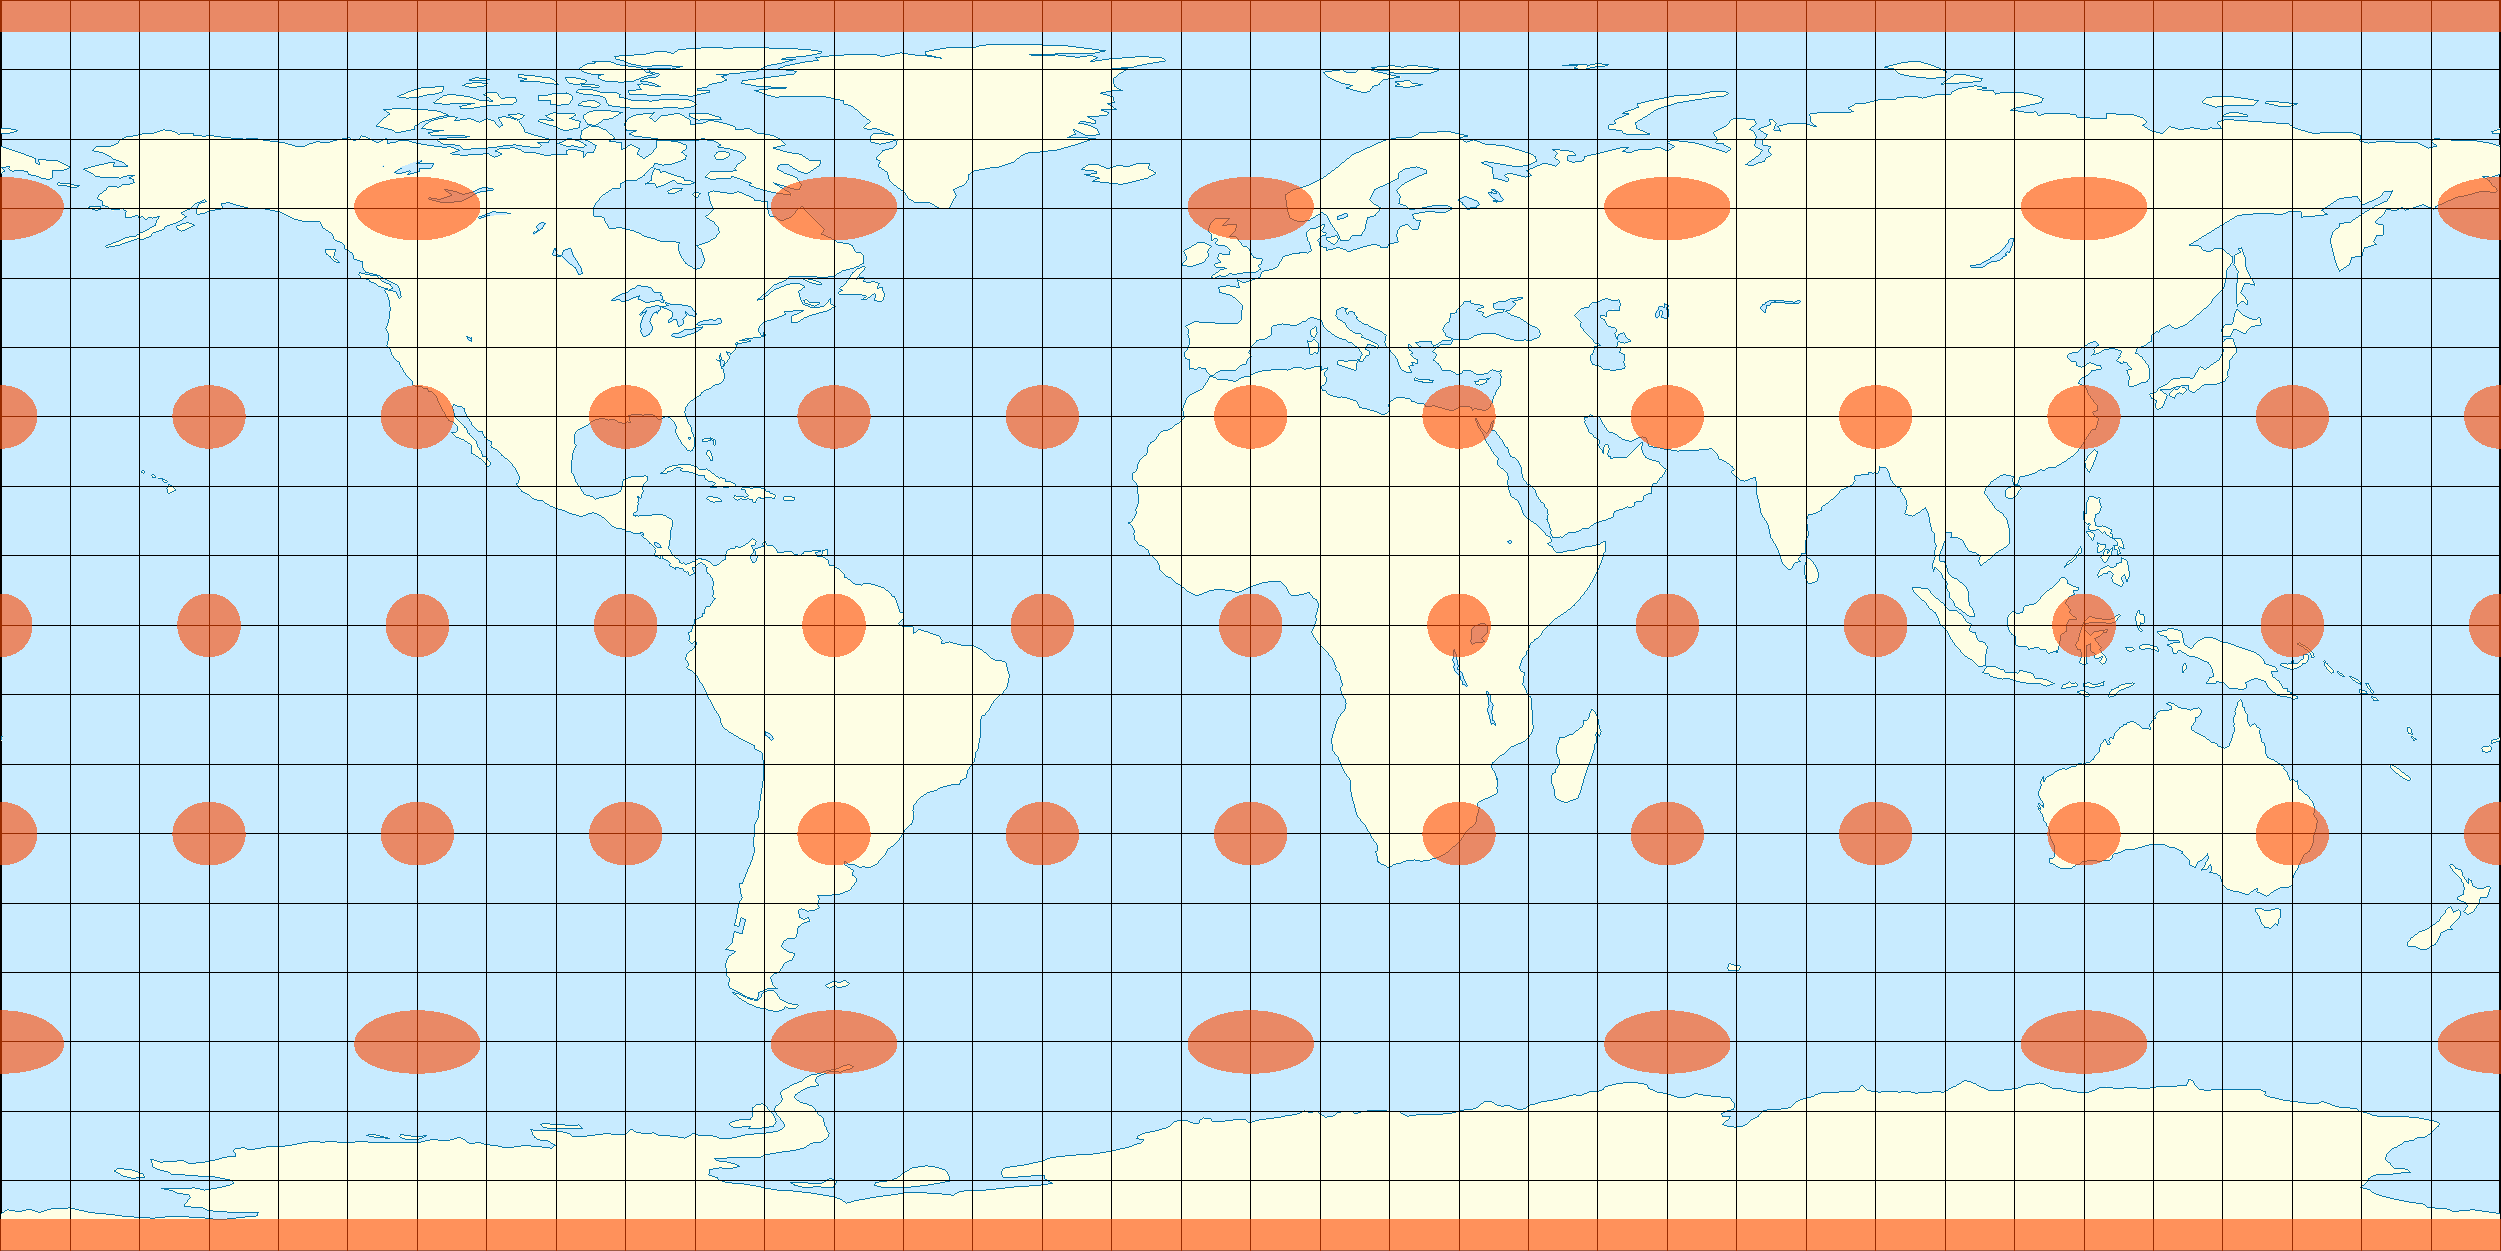
\includegraphics[width=\unitlength,page=1]{plattkarte.pdf}}%
						\end{picture}%
						\endgroup%
						\caption{Verzerrung durch die Plattkarten-Projektion}
						\label{fig:plattkarte}
					\end{figure}
				% end

				\paragraph{Mercator-Projektion}
					Die Mercator-Projektion
					\begin{align}
						x & = \varphi                      &
						y & = \mathrm{arctanh}(\sin\theta)
					\end{align}
					ist die verbreitetste Projektion, da sie winkeltreu ist und dadurch zur Navigation verwendet werden kann. Die Anwendung dieser Projektion auf \autoref{fig:tissot} ist in \autoref{fig:mercator} zu sehen.

					\begin{figure}
						\centering
						\includegraphics[width=0.6\linewidth]{mercator\IfDarkModeT{-dark}}
						\caption{Verzerrung durch die Mercator-Projektion}
						\label{fig:mercator}
					\end{figure}
				% end

				\paragraph{Winkel-Tripel}
					Durch die komplexe Winkel-Tripel-Projektion ist es möglich, eine Flächentreue Darstellung zu erhalten, welche allerdings weder Winkel- noch Längentreu ist. Die Anwendung dieser Projektion auf \autoref{fig:tissot} ist in \autoref{fig:winkeltripel} zu sehen.

					\begin{figure}
						\centering
						\def\svgwidth{\linewidth}
						%% Creator: Inkscape inkscape 0.92.5, www.inkscape.org
						%% PDF/EPS/PS + LaTeX output extension by Johan Engelen, 2010
						%% Accompanies image file 'winkeltripel.pdf' (pdf, eps, ps)
						%%
						%% To include the image in your LaTeX document, write
						%%   \input{<filename>.pdf_tex}
						%%  instead of
						%%   \includegraphics{<filename>.pdf}
						%% To scale the image, write
						%%   \def\svgwidth{<desired width>}
						%%   \input{<filename>.pdf_tex}
						%%  instead of
						%%   \includegraphics[width=<desired width>]{<filename>.pdf}
						%%
						%% Images with a different path to the parent latex file can
						%% be accessed with the `import' package (which may need to be
						%% installed) using
						%%   \usepackage{import}
						%% in the preamble, and then including the image with
						%%   \import{<path to file>}{<filename>.pdf_tex}
						%% Alternatively, one can specify
						%%   \graphicspath{{<path to file>/}}
						%%
						%% For more information, please see info/svg-inkscape on CTAN:
						%%   http://tug.ctan.org/tex-archive/info/svg-inkscape
						%%
						\begingroup%
						\makeatletter%
						\providecommand\color[2][]{%
							\errmessage{(Inkscape) Color is used for the text in Inkscape, but the package 'color.sty' is not loaded}%
							\renewcommand\color[2][]{}%
						}%
						\providecommand\transparent[1]{%
							\errmessage{(Inkscape) Transparency is used (non-zero) for the text in Inkscape, but the package 'transparent.sty' is not loaded}%
							\renewcommand\transparent[1]{}%
						}%
						\providecommand\rotatebox[2]{#2}%
						\newcommand*\fsize{\dimexpr\f@size pt\relax}%
						\newcommand*\lineheight[1]{\fontsize{\fsize}{#1\fsize}\selectfont}%
						\ifx\svgwidth\undefined%
							\setlength{\unitlength}{2250.00002604bp}%
							\ifx\svgscale\undefined%
								\relax%
							\else%
								\setlength{\unitlength}{\unitlength * \real{\svgscale}}%
							\fi%
						\else%
							\setlength{\unitlength}{\svgwidth}%
						\fi%
						\global\let\svgwidth\undefined%
						\global\let\svgscale\undefined%
						\makeatother%
						\begin{picture}(1,0.6111221)%
							\lineheight{1}%
							\setlength\tabcolsep{0pt}%
							\put(0,0){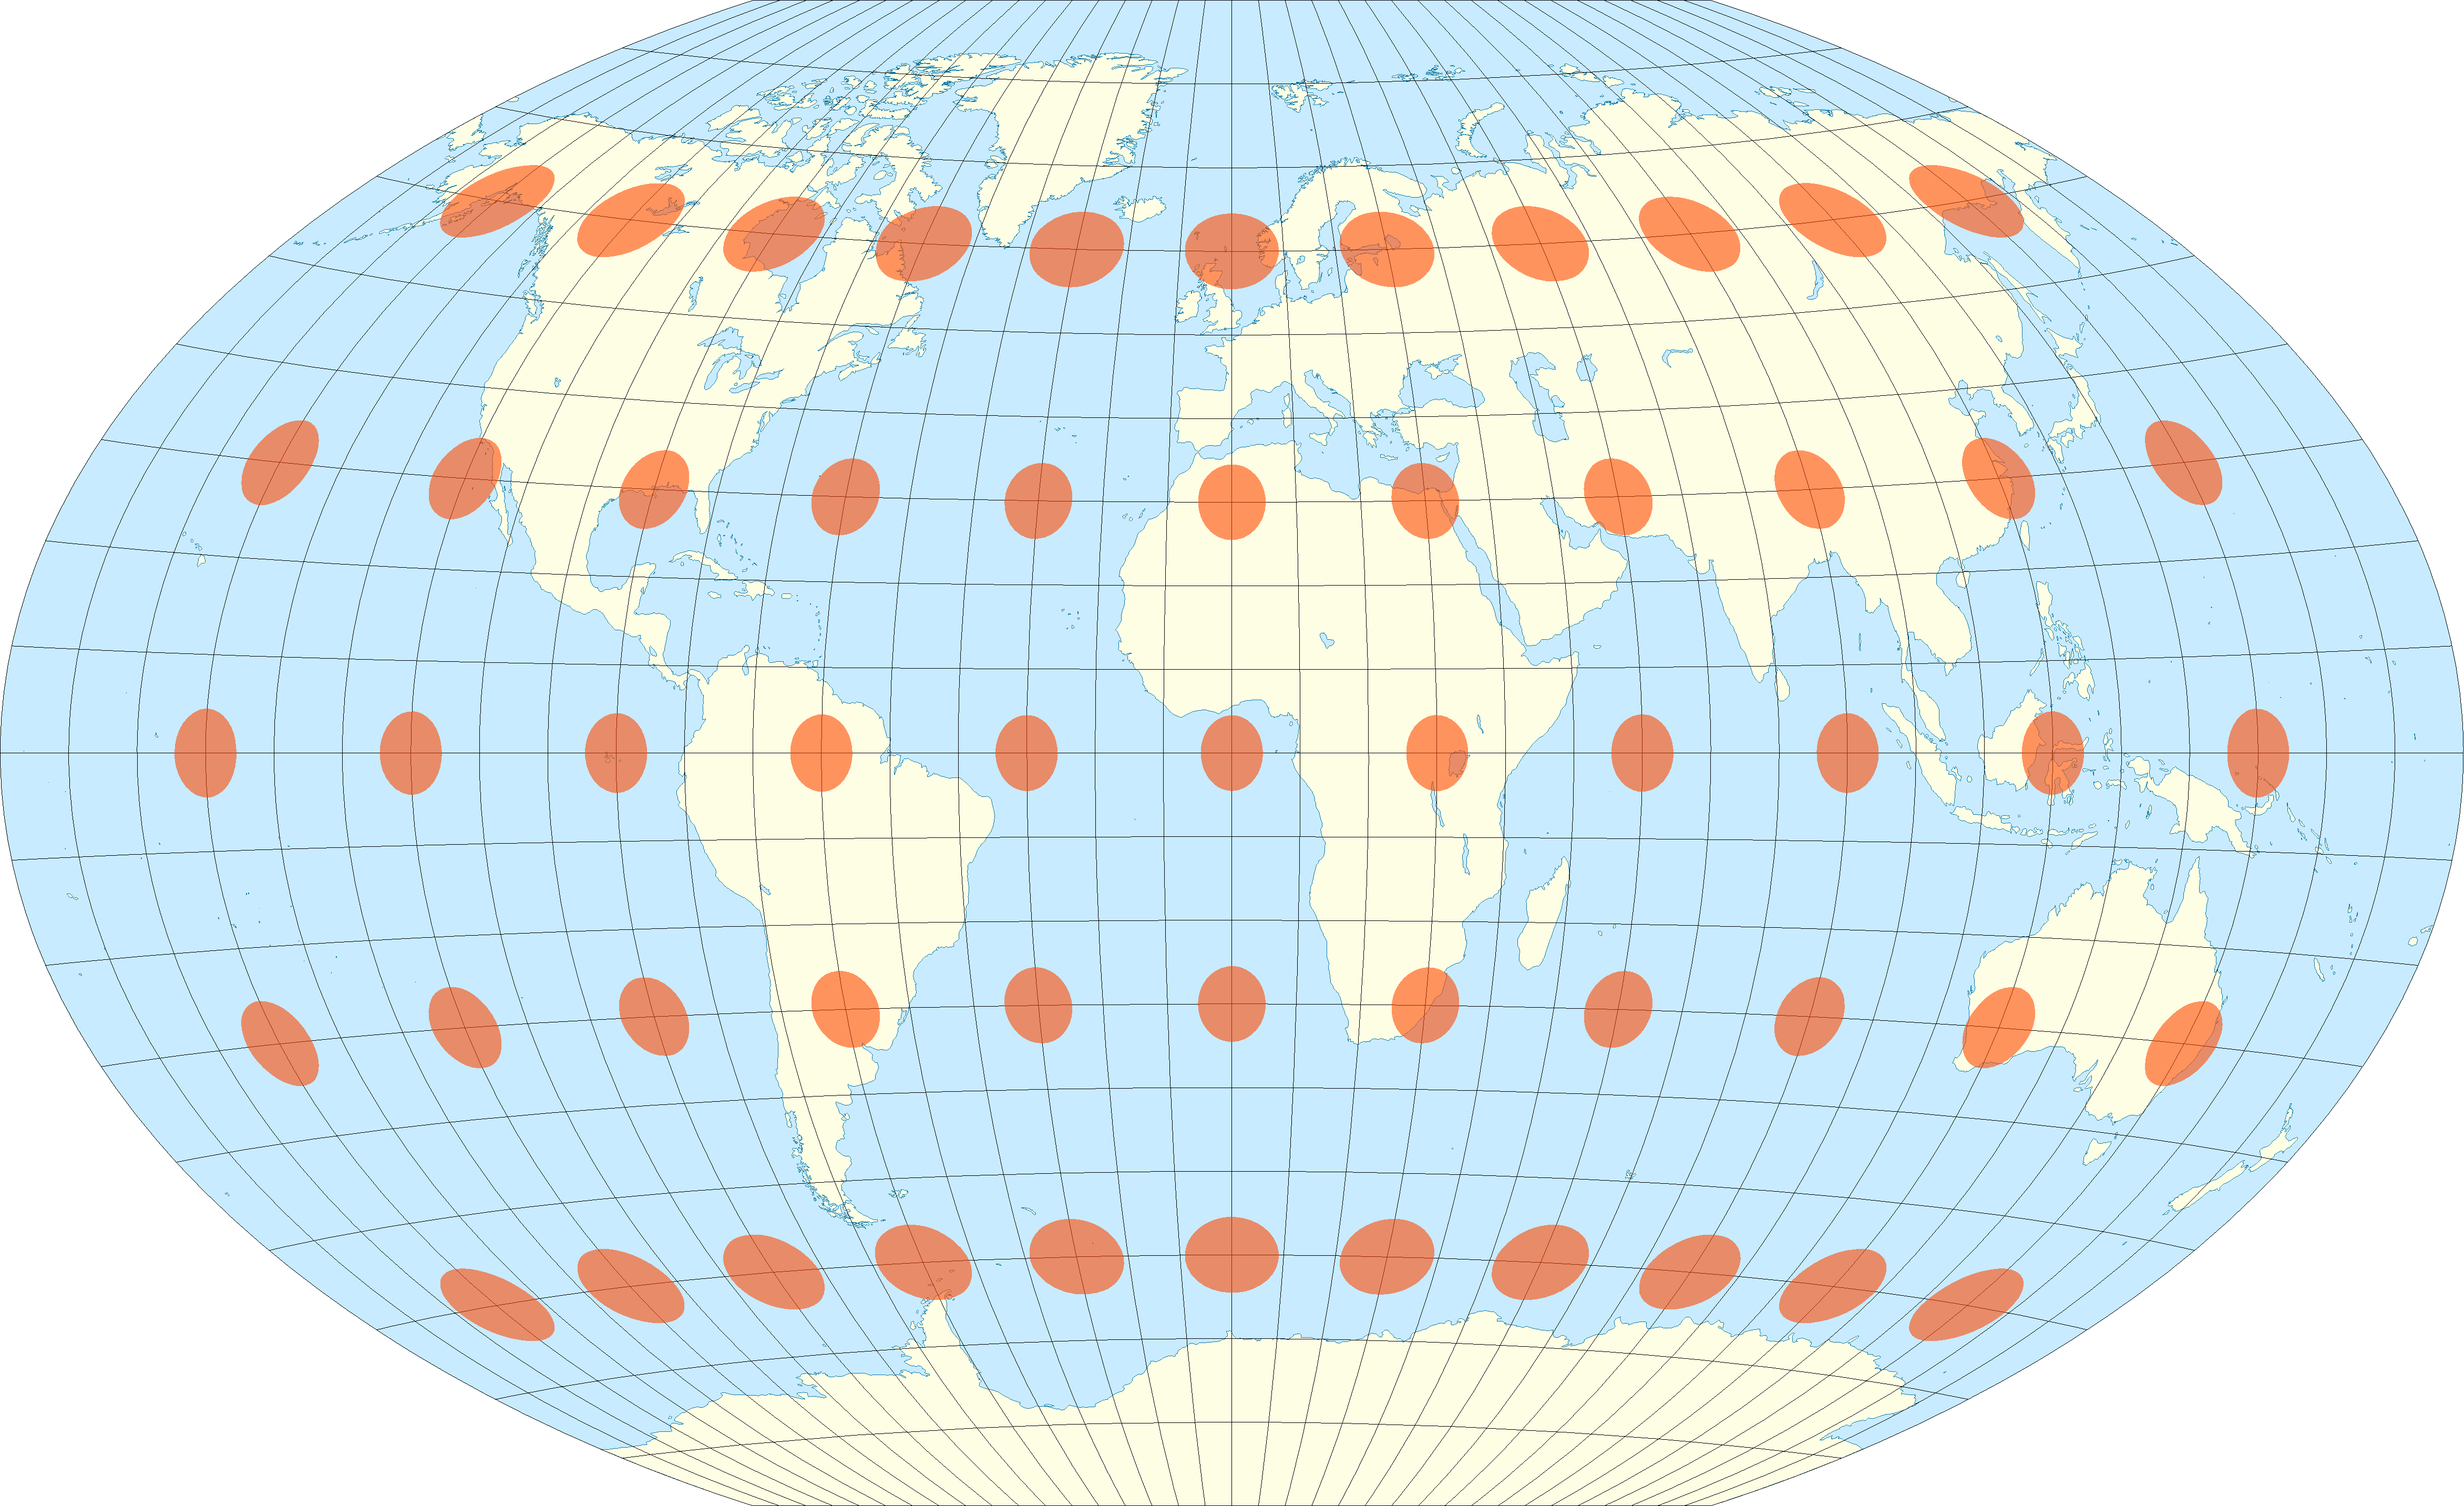
\includegraphics[width=\unitlength,page=1]{winkeltripel.pdf}}%
						\end{picture}%
						\endgroup%
						\caption{Verzerrung durch die Winkel-Tripel-Projektion}
						\label{fig:winkeltripel}
					\end{figure}
				% end
			% end

			\subsubsection{Verzerrte Darstellungen}
				Unter \emph{verzerrte Darstellung} wird eine Visualisierung verstanden, welche getreue Darstellungen bewusst aufgibt, um andere Eigenschaften hervorzuheben\footnote{Achtung: Die Darstellung einer weiteren Eigenschaft auf der Karte, \zB durch Farbe, führt nicht zu einer verzerrten Darstellung! Nur wenn die Darstellung einer Eigenschaft die Positionen der Orte verschiebt ist dies eine verzerrte Darstellung.}. Dabei werden meisten Winkel, Entfernungen und Flächen verzerrt und seltener die Nachbarschaft oder der Wiedererkennungswert. Ein Beispiel aus dem Alltag sind Liniennetzpläne einer U-Bahn, die primär eine Darstellung desselben ist, aber auch versucht, die Nachbarschaft eines Ortes beizubehalten. Dabei wird insbesondere die Entfernung zwischen den Orten verzerrt, um entweder mehr Stationen einfügen zu können oder lange Fahrtzeiten auszublenden.

				Eine weitere Art von verzerrten Karten sind Kartogramme, die eine geografische Karte verzerren. Ein Beispiel ist in \autoref{fig:worldmap} zu sehen. Um eine solche Karte zu erstellen wird ein Gitter über die "echten" Raumkoordinaten gelegt und die Knoten gewichtet. Dadurch werden benachbarte Gitterknoten in leere Bereiche gedrückt, bis eine monotone "Gewichtsverteilung" entsteht (dies kann unter anderem den Flächenbias reduzieren, da die Fläche nun tatsächlich die Daten abbildet). Zur Einteilung von Kartogrammen gibt es verschiedene Kriterien, \zB stetig/diskret und der Grad der Form- und Nachbarschaftserhaltung (dabei sollen auch "nicht-Nachbarschaften" erhalten bleiben). Als sehr weit gefasste Karte können dies auch Small Multiples sein, die grob in eine geografische Ordnung gebracht werden (\zB für jedes Bundesland eine Grafik).

				\begin{figure}
					\centering
					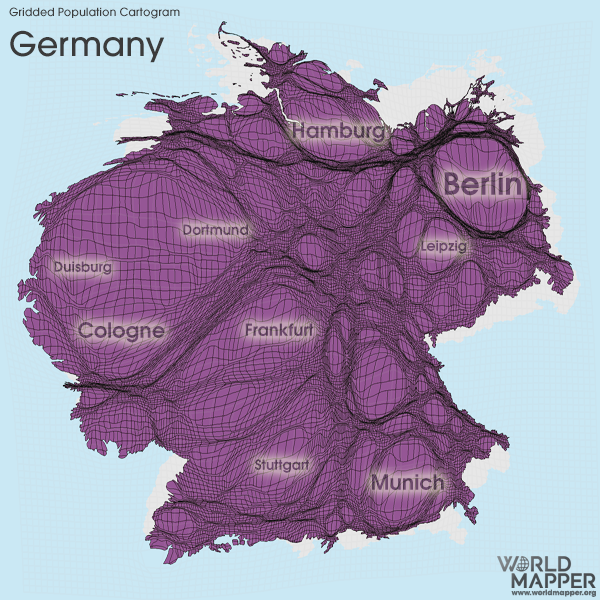
\includegraphics[width=0.6\linewidth]{worldmapper}
					\caption[Beispiel für eine verzerrte Karte]{Auf dieser verzerrten Karte wird die Wähler*innenpopulation der Bundestagswahl 2021 dargestellt, wobei die Karte so verzerrt wurde, dass sie die Wähler*innendichte darstellt (\dh eine Flächeneinheit enthält die gleiche Anzahl Wähler*innen unabhängig von dessen Position). Das Gitter wurde über die Karte gelegt um die Richtung der jeweiligen Ausdehnung hervorzuheben.}
					\label{fig:worldmap}
				\end{figure}
			% end
		% end

		\subsection{Nicht-Ortsbezogene Daten}
			Die Darstellung nicht-ortsbezogener Daten kann \zB sinnvoll sein, um die bestehenden Intuitionen auszunutzen. Das größte Problem ist dabei die Festlegung des Ortes, also die Abbildung der Daten auf zwei Koordinaten und die Auswahl relevanter Landmarken zur Orientierung. Für ersteres können sämtlich besprochenen Verfahren zur Dimensionsreduktion (\autoref{subsubsec:dimred}) und Graph-Layouting (\autoref{sec:visGraphen}) genutzt werden.

			Weitere Herausforderungen sind (eventuell) die Konstruktion einer Topographie, die im Hintergrund dargestellt werden kann und die Wahl geeigneter Metaphern um Informationen und Beziehungen effektiv und konsistent zu übersetzen.
		% end

		\subsection{Raum-Zeit Daten}
			Bei der Darstellung von orts- und zeitbezogenen Daten müssen drei Attribute (zwei für den Raum und eine für die Zeit) in einer Visualisierung untergebracht werden, welche sonst üblicherweise auf die Position abgebildet werden. Die einfachste Variante dafür ist ein 3D-Diagramm, was allerdings schnell unübersichtlich werden kann.

			Für andere Arten von Visualisierungen wird angenommen, dass Bewegung stetig im Raum sind (\dh Punkte dürfen verbunden werden) und durch Trajektorien beschrieben werden. Unter dieser Annahme ist es möglich, Bewegungsdaten nur zweidimensional Aufzutragen und die Bewegungsrichtung zu markieren (wenn es nicht zu viele Überschneidungen gibt oder Trajektorien gibt; wobei dies durch Interaktion und Bundling abgeschwächt werde kann). Soll die Geschwindigkeit dargestellt werden, kann dies \bspw über Farbe passieren.
		% end
	% end
% end

\chapter{Visual Analytics}
	In den vorherigen Kapitel wurde der erste Teil, die Informationsvisualisierung, behandelt. Dabei ging es darum, wie Daten dargestellt werden. In der Visual Analytics, diesem Kapitel, geht es hingegen darum, wie eine Visualisierung für die Analyse genutzt werden kann und umgekehrt. Die Informationsvisualisierung ist also nur eine Komponente. Allerdings ist sie mehr als nur eine Visualisierung von Ergebnissen, sondern die automatische Modellierung und die Visualisierung bestehen gleichberechtigt nebeneinander und werden für verschiedene Teilaufgaben verwendet.

	\section{Definition}
		Für die Visual Analytics gibt es im Grunde zwei große Definition, wobei die zweite sehr viel Allgemeiner ist:
		\begin{itemize}
			\item "Visual Analytics ist die Kombination automatischer Analysetechniken mit interaktiven Visualisierungen um große und komplexe Daten zu verstehen und auf deren Basis Entscheidungen treffen zu können." (Keim et al., 2008)
			\item "Visual Analytics ist die Wissenschaft des analytischen Schließens, unterstützt durch interaktive, visuelle Schnittstellen." (Thomas und Cook, 2005)
		\end{itemize}
		Diese beiden Definitionen und ihre Bedeutung werden nun genauer beleuchtet.

		\subsection{Definition nach Keim et al.}
			Die erstere, ältere, vereint zwei wichtige Vorgänger der Visual Analytics, die \emph{Informationsvisualisierung}\footnote{"Nutzung von computerunterstützten, interaktiven, visuellen Repräsentierungen abstrakter Daten mit dem Ziel, das Erkenntnisvermögen zu verbessern" (Card et al., 1999)} und die \emph{Knowledge Discovery (in Databases)}\footnote{"nicht-trivialer Prozess für die Suche nach validen, neuen, potentiell relevanten und nutzbaren Mustern in Datenbeständen" (Fayyad et al., 1996)} (KDD). Um diese Definition im Detail zu verstehen, ist es zunächst wichtig, das KDD-Modell zu verstehen.

			\subsubsection{Der Knowledge Discovery Prozess und das KDD-Modell}
				Das KDD-Modell stellt, ähnlich wie der Informationsvisualisierungsprozess, den Prozess der \emph{Knowledge Discovery}, also dem Entdecken von Wissen, in einer einfachen Pipeline dar (siehe \autoref{fig:kdd}). Im Folgenden werden die einzelnen Schritte des Modells im Detail beschrieben:
				\begin{enumerate}
					\item Im ersten Schritt (\emph{Kennenlernen der Anwendungsdomäne}) muss die Anwendungsdomäne im Detail kennen gelernt werden. Dies bedeutet, dass die Daten und die Fragestellung gesichtet werden müssen. Des weiteren wird die Relevanz der Daten sowie die der Zwischenergebnisse und die Analyse beurteilt und die Fragestellung der Anwendung wird in die Analyse übersetzt. Hierbei können bereits kleinere Visualisierungen angewendet werden, \zB um die Rohdaten anzuschauen.
					\item Im zweiten Schritt (\emph{Auswahl der Daten}) müssen die Daten zu Weiterverwendung selektiert werden. Dies geschieht auf verschiedensten Kriterien, \zB Relevant, Repräsentativität, Vollständigkeit ("Sauberkeit"), Verfügbarkeit und eventuellen Kosten.
					\item Anschließend müssen die Daten, wie bei der Informationsvisualisierung, vorverarbeitet werden (\emph{Datenvorverarbeitung}). Dabei können alle aus \autoref{sec:dataTransformation} bekannten Verfahren angewendet werden.
					\item Im vierten Schritt wird die Data-Mining-Aufgabe bestimmt (\emph{Bestimmung der Data-Mining-Aufgabe}), \dh ob ein Clustering-, Klassifikations, Regressions- oder ein anderes Problem vorliegt.
					\item Basierend auf der im vierten Schritt identifiziert Aufgabe wird nun ein passendes Verfahren gewählt (\emph{Auswahl des Data-Mining-Verfahrens}). Hierfür stehen hunderte Verfahren zur Verfügung, von denen in \autoref{sec:dataMining} einige vorgestellt werden.
					\item Vor Anwendung des Verfahrens müssen die Daten eventuell erneut vorverarbeitet und an die Anforderungen der Methode angepasst werden (\emph{Datentransformation und Reduktion}). Dieser Schritt ist neben der ursprünglichen Vorverarbeitung der aufwendigste Schritt und kann \zB Verfahren zur Dimensionsreduktion beinhalten.
					\item Im siebten Schritt wird das Data-Mining-Verfahren tatsächlich angewendet. Dies inkludiert die Auswahl passender Parameter und Qualitätskriterien. Das Ergebnis sind Muster und/oder Modelle.
					\item Im abschließenden Schritt werden die Ergebnisse gesichtet, getestet und zur Vermittlung an den*die Anwender*in aufbereitet (insbesondere werden die Ergebnisse in den Kontext der Aufgabe gesetzt). Es ist alternativ auch möglich, die Daten (automatisiert) weiter zu verwenden.
				\end{enumerate}

				\begin{figure}
					\centering
					\tikzKdd
					\caption{Das Knowledge Discovery Prozess-Modell}
					\label{fig:kdd}
				\end{figure}
			% end

			\subsubsection{Gemeinsamkeiten zwischen dem KDD-Modell und dem Visualisierungsprozess}
				Beide Modelle -- das KDD-Modell und der Visualisierungsprozess -- sind Datenflussmodelle, bei denen die Schritte interaktiv und iterativ ab, \dh die Schritte können wiederholt werden und das Wissen am Ende der jeweiligen Pipeline wird nicht (vollständig) automatisch generiert. Weitere Gemeinsamkeiten sind die Vorverarbeitung und die Interpretation/Evaluation durch den Menschen mit dem Ziel des (Aufgaben-bezogenen) Erkenntnisgewinns. Die charakteristischen Schritte des jeweiligen Prozesses sind die visuelle Abbildung, View Transformation und das Ergebnis als "Bild" bei der Informationsvisualisierung und der Einsatz von Data-Mining-Verfahren im KDD-Modell, wobei die Darstellung der Ergebnisse nicht strikt definiert ist.
			% end
		% end

		\subsection{Definition nach Thomas und Cook}
			Die zweite Definition von Visual Analytics als \emph{Wissenschaft des analytischen Schließens} ist sehr viel Allgemeiner und beschreibt dabei die Herleitung von Entscheidungen aus empirischen Daten, die Falsifikation/Bestätigung von Hypothesen und die Entwicklung von Methoden zur Herleitung (\bspw Data-Mining, Simulation, Präsentation, etc.). Das übergreifende Ziel ist dabei die nachvollziehbare Verknüpfung aller elementaren Daten. Eine Illustration dieses Konzepts mit einzelnen Schritten ist in \autoref{fig:cook} zu sehen. Technologien der Visual Analytics bewegen sich dabei auf zwei Achsen zwischen der Findung eines Modells und der Visualisierung sowie den Ebenen des Modells von Thomas und Cook (siehe \autoref{fig:va}).

			\begin{figure}
				\centering
				\begin{tikzpicture}[<->, every node/.style = { draw, rectangle, minimum height = 0.75cm, minimum width = 5cm }]
					\node (a) {Szenario, Entscheidung};
					\node [below = 0.75 of a] (b) {Hypothesen, Empfehlungen};
					\node [below = 0.75 of b] (c) {Argumente, Modelle};
					\node [below = 0.75 of c] (d) {Muster};
					\node [below = 0.75 of d] (e) {Elementare Daten};

					\draw (a) to (b);
					\draw (b) to (c);
					\draw (c) to (d);
					\draw (d) to (e);
				\end{tikzpicture}
				\caption{Illustration der Schritte der "Wissenschaft des analytischen Schließens"}
				\label{fig:cook}
			\end{figure}

			\begin{figure}
				\centering
				\includegraphics[width=\linewidth]{va\IfDarkModeT{-dark}}
				\caption[Die zwei Achsen der Visual Analytics]{Die zwei Achsen der Visual Analytics\\Quelle: Vorlesungsfolien}
				\label{fig:va}
			\end{figure}
		% end
	% end

	\section{Das Visual Analytics Prozessmodell}
		Bereits im KDD-Prozess werden Visualisierungen für die Sichtung von (Zwischen-) Ergebnissen genutzt, wobei die Verfahren häufig nebeneinander und strikt getrennt verwendet werden. In der Visual Analytics wird diese strikte Trennung aufgebrochen und stattdessen eine direkte Verbindung hergestellt (siehe \autoref{fig:direkteVerbindung}). Diese \emph{direkte Verbindung} ist das Herzstück der modernen Visual Analytics, während die "alte" Vorgehensweise nur die indirekte Verbindung ausweist. Es kann im neuen Modell \zB die Interaktion mit einer Visualisierung das Modell beeinflussen.

		Da sich über eine Reiteration jede direkte Kopplung auch als eine indirekte Kopplung realisieren kann, wirkt die Unterscheidung zunächst arbiträr. Diese kann klar definiert werden: Findet zwischen zwei Techniken ein direkter Datenfluss oder -austausch statt, so ist die Kopplung \emph{direkt}, sonst \emph{indirekt}. Bei einer indirekten Kopplung muss der*die Nutzer*in zwischen dem Output und dem erneuten Input also händisch eingreifen. Bei einer direkten Kopplung genügt es hingegen, die Daten neu zu laden ohne irgendwie einzugreifen. Im Idealfall ist dies sogar transparent, sodass nur mit der Visualisierung gearbeitet werden muss.

		\begin{figure}
			\centering
			\begin{tikzpicture}[->, cmp/.style = { draw, rectangle, minimum height = 0.75cm, minimum width = 3cm }]
				\node (eingabe) {Eingabe};
				\node [cmp, right = 1cm of eingabe] (daten) {Daten};
				\node [cmp, right = 2cm of daten, yshift =  1.25cm] (visualisierung) {Visualisierung};
				\node [cmp, right = 2cm of daten, yshift = -1.25cm] (modell) {Modell};
				\node [cmp, right = 2cm+3cm+2cm of daten] (erkenntnis) {Erkenntnis};
				\draw (eingabe) to (daten);
				\draw (daten.east) to[out = 0, in = 180] (visualisierung.west);
				\draw (daten.east) to[out = 0, in = 180] (modell.west);
				\draw (visualisierung.east) to[out = 0, in = 180] (erkenntnis.west);
				\draw (modell.east) to[out = 0, in = 180] (erkenntnis.west);
				\draw [<->, TUDa-9c] (visualisierung) to node[fill = white]{\textbf{Direkte Verbindung}} (modell);
				\coordinate [below = 3.5 of erkenntnis] (a);
				\draw [dashed] (erkenntnis) to (a) -| coordinate(b) (eingabe);
				\path (a) to node[above]{Indirekte Verbindung} (b);
				\draw (visualisierung.east) to[out = 0, in = 90, looseness = 3] node[above, yshift = 0.2cm]{Informationsvisualisierung} (visualisierung.north);
				\draw (modell.east) to[out = 0, in = -90, looseness = 3] node[below, yshift = -0.3cm]{Knowledge Discovery} (modell.south);
			\end{tikzpicture}
			\caption{Das Visual Analytics Prozessmodell}
			\label{fig:direkteVerbindung}
		\end{figure}
	% end

	\section{Stärken und Schwächen von Mensch und Maschine}
		Da das Hauptziel der Visual Analytics die Verbesserung von automatischen Verfahren durch Visualisierung und anders herum ist, muss zunächst verstanden werden, was die Stärken und Schwächen von Mensch und Maschine ist und wo ein automatisches Verfahren dem Menschen oder ein Mensch dem automatischen Verfahren helfen kann. Dabei ist die eigentliche zentrale Frage
		\begin{center}
			Was ist ein Muster?
		\end{center}
		Diese Frage wird von verschiedenen Menschen und automatischen Verfahren sehr unterschiedlich beantwortet und ist, da automatische Verfahren insbesondere Muster finden sollen, sehr relevant um Verbesserungen und Hilfestellungen zu identifizieren.

		Im Rahmen des KDD-Modells wurde die folgende Definition eines Musters vorgeschlagen: "Ausdruck in einer formalen Sprache oder ein Modell, das eine Teilmenge aller Datensätze beschreibt" (Fayyad et al., 1996). In anderen Worten ist ein Muster also eine nicht zufällige Teilmenge von Daten (\zB formal ausgedrückt durch SQL-Queries, algebraische Ausdrücke oder periodische Folgen als Teilmenge aller Ziffernfolgen). Diese Definition setzt allerdings eine formale Beschreibung eines Musters voraus, es gibt allerdings auch Daten, die keiner formalen Definition genügen, aber allgemein auch als Muster anerkannt sind, \zB Design Patterns in der Softwareentwickler, die Menge aller Bauwerke, die "Haus" genannt werden, die Menge aller Bekannten, die als "Freunde" bezeichnet werden, die Menge aller Musikstücke, die einer Person gefallen, uvm.. Diese Muster sind für die Datenanalyse oft interessanter, da sie real existierende Dinge darstellen. Allerdings sind sie auch um ein vielfaches schwerer, da ein Mensch es oftmals nicht schafft, eine formale Definition zu finden.

		Eine weitere Definition eines Musters, die insbesondere in der Informationsvisualisierung relevant ist, ist: "Ein visuelles Muster ist ein \emph{subjektiver} Sinneseindruck, der Informationen über \emph{mehrere} Elemente eines Bildes zusammenfasst". Nach dieser Definition muss sich ein Muster also nicht unbedingt wiederholen, noch muss es zusammenhängend oder formal definiert sein.

		Unabhängig von der genauen Definition kann sich allerdings auf einige Eigenschaften von Mustern geeinigt werden, die sowohl in der Informationsvisualisierung als auch im KDD-Modell gelten:
		\begin{enumerate}
			\item Ein Muster ist eine Teilmenge einer Grundmenge (\zB die Menge aller Bauwerke).
			\item Ein Muster hat \emph{mehr als ein} Element und enthält \emph{nicht alle} Elemente.
			\item Ein Muster wird nicht als Zufall erfasst/berechnet/gesehen/gelernt/vermutet/etc..
		\end{enumerate}
		Dabei gibt es Modell- und nicht-Modellbasierte Muster. Ein Modell kann dabei verschieden ausgeprägt sein, \bspw ein Beschreibungsmodell, welches es ermöglicht, Muster zu unterscheiden oder ein Prognosemodell, welches es ermöglicht, auch vorher unbekannte Instanzen zuzuordnen. Bei der Knowledge Discovery werden Muster dabei fast immer zusammen mit einem Modell erzeugt, welches dieses Muster beschreibt.

		Ein Überblick über die verschiedenen und gemeinsamen Eigenschaften eines Musters in der Informationsvisualisierung und im KDD-Prozess ist in \autoref{tab:muster} gegeben.

		\begin{table}
			\centering
			\begin{tabular}{l|l}
				\toprule
				\textbf{Informationsvisualisierung}         & \textbf{Knowledge Discovery}  \\ \midrule
				Sinneseindruck                              & Ausdruck in formaler Sprache  \\
				ohne Modell definiert                       & durch ein Modell spezifiziert \\
				räumlich begrenzter Bereich des Sichtfeldes & (lesbar)                      \\
				subjektiv                                   & objektiv                      \\
				nicht formalisiert                          & reproduzierbar                \\
				nicht (direkt) kommunizierbar               & "nachweisbar nicht zufällig"  \\
				\multicolumn{2}{c}{Zusammenfassung mehrere Datensätze zu einem Artefakt}    \\ \bottomrule
			\end{tabular}
			\caption{Verschiedene/Gemeinsame Eigenschaften eines "Musters" in Informationsvisualisierung und Knowledge Discovery}
			\label{tab:muster}
		\end{table}

		\subsection{Mensch vs. Maschine}
			Wenn ein Mensch ein Muster erkennen soll, so ist eine geeignete Visualisierung notwendig, da Menschen primär in Bildern Muster erkennen. Dadurch können auch Muster gefunden werden, die vorher nicht spezifiziert wurden und es kann die Erkennung komplexester Muster gelernt werden. Daraus folgt allerdings, dass die Ergebnisse stark von dem*der Anwender*in abhängen, nicht direkt nutzbar und deterministisch sind. Soll hingegen eine Maschine ein Muster erkennen, so ist ein formaler Algorithmus notwendig. Die Entwicklung eines solchen Algorithmus ist jedoch schwierig und grenzt den Suchraum bereits durch das Design stark ein. Allerdings ist das Ergebnis eine formale, nutzbare Beschreibung des Musters. Diese Divergenz in den Anforderungen hat verschiedene Vor- und Nachteile, die sich in den Schwächen von Mensch und Maschine widerspiegeln. Eine Übersicht dieser ist in \autoref{tab:staerken} gegeben. In den folgenden Abschnitten werden die Schwächen genauer beleuchtet, da diese zu den Kernpunkten der Visual Analytics führen.

			\begin{table}
				\centering
				\begin{tabular}{l|l}
					\toprule
					\textbf{Stärken des Menschen}                      & \textbf{Stärken der Maschine}         \\ \midrule
					flexible, robuste Wahrnehmung                      & Kontrollierbarkeit                    \\
					Mustererkennung unter schwierigsten Bedingungen    & Wiederholbarkeit                      \\
					Wahrnehmung ungewöhnlicher/unerwarteter Ereignisse & großer Arbeitsspeicher                \\
					Datenunsicherheit                                  & Deduktives Schließen                  \\
					Kreativität                                        & Schnelligkeit                         \\
					Langzeitgedächtnis, Weltwissen                     & Präzision                             \\
					Urteilskompetenz                                   & Zuverlässigkeit                       \\
					(Induktives Schließen)                             & Multitasking                          \\
					Abduktives Schließen (Hypothesenbildung)           & Ausdauer                              \\ \midrule
					\textbf{Schwächen des Menschen}                    & \textbf{Schwächen der Maschine}       \\ \midrule
					kleines Arbeitsgedächtnis                          & Rauschen                              \\
					sequentielle, sprachliche Verarbeitung             & Mehrdeutigkeit                        \\
					hochdimensionalen Daten                            & Datenunsicherheit                     \\
					geringe Ausdauer                                   & Formale Beschreibung notwendig        \\
					Abhängigkeit von äußeren Einflüssen                & sehr begrenze Anpassung an neue Reize \\
					Nichtreproduzierbarkeit                            & \emph{sehr} hochdimensionale Daten    \\
					Abduktives Schließen (Falsche Prämissen)           &
				\end{tabular}
				\caption{Stärken und Schwächen von Mensch und Maschine}
				\label{tab:staerken}
			\end{table}

			\subsubsection{Schwächen des Menschen}
				Das Arbeitsgedächtnis eines Menschen ist sehr klein und kann zur selben Zeit nur drei bis fünf Informationselement bereit halten. Dadurch können komplexe Zusammenhänge nicht ohne Hilfsmittel zusammengeführt und erkennt werden, was die Interpretation von Mustern beeinflusst. Ebenso sind die Ergebnisse nichtreproduzierbar, da Sinneseindrücke nicht sprachlich fixiert und formalisiert sind. Eine Formalisierung wird erst nach der Interpretation "künstlich" eingefügt. Da das Denken außerdem in 2D/3D verankert ist, können Menschen im Allgemeinen schlecht mit hochdimensionalen Daten umgehen, da die hier auftretenden Effekten der Intuition widersprechen und dadurch schwer vorstellbar sind.
			% end

			\subsubsection{Schwächen der Maschine}
				Die Schwächen einer Maschine sind, annähernd komplementär zu den Schwächen eines Menschen. So kann eine Maschine \bspw schlecht mit Mehrdeutigkeiten umgehen und erstellt eher eine Beschreibung eines sehr komplexen Musters statt drei einfache Muster zu erkennen. Außerdem können Datenpunkte sogar zu mehreren Mustern gehören, was das Problem nochmal komplexer macht. Des weiteren sind Maschinen schlecht darin, mit Rauschen und Unsicherheiten umzugehen und falsche Daten führen eher zu komplexeren Modellen statt dem Eliminieren einzelner Datenpunkte als Ausreißer. Ferner schränkt bereits die Wahl des Data-Mining-Verfahrens die erkennbaren Muster ein: Kann ein Modell \bspw gut Rechtecke beschreiben, wird die Beschreibung eines Kreises schwer und umgekehrt.

				Zusammengefasst werden viele dieser Symptome als \emph{Okchams Dilemma:}
				\begin{center}
					"Keine formale Sprache ist in der Lage, in \emph{jedem} Fall gleichzeitig das genauste \emph{und} einfachste Modell zu repräsentieren."
				\end{center}
			% end
		% end

		\subsection{Ähnlichkeit}
			Eine der Hauptkomponenten bei der Mustererkennung (insbesondere dem Finden von Gruppierungen) ist die Definition einer \emph{Ähnlichkeit}. Die Definition einer solchen Ähnlichkeit und die entsprechende Anordnung ist allerdings extrem schwer und baut bei Menschen häufig auf das Objekt selbst und Vorwissen und Interessen des*der Nutzers*Nutzerin auf. Daher ist die Ähnlichkeit auch häufig nicht deterministisch\dots~Für Data-Mining-Verfahren muss die Ähnlichkeit häufig als ein \emph{Distanzmaß} \( \mathrm{dist}(\vec{x}, \vec{y}) \) zwischen zwei Datenpunkten \(x\) und \(y\) definiert werden. Dies kann \zB die \emph{Manhatten-}, \emph{Euklidische-} oder \emph{Maximums-Distanz} (in dieser Reihenfolge):
			\begin{align}
				d_1(\vec{x}, \vec{y})      & = \sum_i \lvert x_i - y_i \rvert &
				d_2(\vec{x}, \vec{y})      & = \sqrt{\sum_i (x_i - y_i)^2}    &
				d_\infty(\vec{x}, \vec{y}) & = \max_i \lvert x_i - y_i \rvert
			\end{align}
			Viele andere Distanzmaße können in der \emph{Enzyklopädie der Distanzen} (ISBN-13: 978-3-662-52844-0) gefunden werden.

			Eine andere Möglichkeit zur Distanzrepräsentation ist die explizite Auflistung dieser in einer Matrix. Diese \emph{Ähnlichkeitsmatrix} enthält dann alle Distanzen für jedes Punktepaar. Während dieser Ansatz Vorwissen auch ohne explizite mathematische Modellierung abbilden kann, damit sehr flexibel ist und die Datenpunkte auch keine Attribute benötigen, kann er einige Problem hervorrufen. Zunächst steigt der Speicherverbrauch quadratisch mit der Anzahl der Datenpunkte. Des weiteren ist nicht garantiert, dass die so definierte Ähnlichkeit tatsächlich eine Metrik ist (Dreiecksungleichung), weshalb manche Verfahren zusammenbrechen können. Außerdem ist ein Clustering so möglicherweise schon durch den Menschen vorgegeben und die Stärken der Maschine werden nicht verwendet.

			Die erste Aufgabe zur Anwendung von Data-Mining-Verfahren besteht also in der Wahl einer geeigneten Ähnlichkeitsmetrik, die die Anforderungen und Fragestellungen des*der Fachexperten*Fachexpertinnen möglichst gut abbildet. Dabei kann es hilfreich sein, die Expert*innen zunächst zu befragen, \bzw sie Daten manuell sortieren zu lassen, um eine Idee für die relevanten Aspekte zu bekommen. Anschließend sollte auch beim durchlaufen des KDD-Modells immer Rücksprache gehalten und Zwischenergebnisse diskutiert werden. So kann es \bspw passieren, dass eine Diskretisierung oder Entrauschung wichtige Details entfernt, sodass das angeschlossene Modell gar keine korrekten Antworten mehr geben kann. Es sollte also immer die formale Ähnlichkeit in Form einer Formel mit der informellen Ähnlichkeit in Form der Meinung eines*einer Expert*in sichergestellt werden, wobei die (Zwischen-) Ergebnisse visualisiert werden müssen.
		% end
	% end

	\section{Automatische Verfahren}
		\label{sec:dataMining}

		Um die Verbesserung automatischer Verfahren behandeln zu können, ist es zunächst hilfreich, eine Idee davon zu bekommen, wie diese Verfahren arbeiten. Dabei gehen die meisten Verfahren ähnliche Schritte durch, die in \autoref{fig:autoVerfahren} gezeigt sind. Die meisten Verfahren werden dabei zur Extraktion von Mustern und Erstellung von Modellen genutzt. Im Folgenden werden einige Grundbegriffe und Verfahren behandelt, denen im weiteren Verlauf dieses Kapitels einige Erweiterungen hinzugefügt werden, um sie mit Visualisierung und Interaktion zu verbinden.

		\todo{Visual Analytics: Automatische Verfahren} \emph{Ich habe diesen Abschnitt erst einmal ausgelassen, da ich sehr knapp in der Zeit bin und das meiste eh schon bekannt ist aus anderen Zusammenfassungen und Veranstaltungen (siehe \zB \href{https://fabian.damken.net/summaries/cs/elective/iws/dmml}{\emph{Data Mining und Maschinelles Lernen}}\footnote{\url{https://fabian.damken.net/summaries/cs/elective/iws/dmml}} oder \href{https://fabian.damken.net/summaries/cs/elective/vc/statml}{\emph{Statistical Machine Learning}}\footnote{\url{https://fabian.damken.net/summaries/cs/elective/vc/statml}}).}

		\begin{figure}
			\centering
			\begin{ivvaIntegration}
			\end{ivvaIntegration}
			\caption[Grundlegende Schritte automatischer Verfahren]{Darstellung der grundlegenden Schritte von automatischen Verfahren. Das Zwischenergebnis hat dabei häufig, aber nicht immer, die gleiche Form wie das Ergebnis, wird allerdings iterativ verändert. Hat es dir gleiche Form, so können die selben Visualisierungstechniken für das Zwischenergebnis wie für das Ergebnis angewendet werden.}
			\label{fig:autoVerfahren}
		\end{figure}

		\subsection{Grundbegriffe}
			\todo{Visual Analytics: Automatische Verfahren: Grundbegriffe; 12.16, 12.18}  Folien: 12.16, 12.18

			\subsubsection{Clustering und Dimensionsreduktion}
				\todo{Visual Analytics: Automatische Verfahren: Grundbegriffe: Clustering und Dimensionsreduktion; 11.18, 11.19, 11.21, 11.22, 11.23, 11.24, 11.28}  Folien: 11.18, 11.19, 11.21, 11.22, 11.23, 11.24, 11.28
			% end

			\subsubsection{Klassifikation}
				\todo{Visual Analytics: Automatische Verfahren: Grundbegriffe: Klassifikation; 12.13, 12.14, 12.15, 12.17}  Folien: 12.13, 12.14, 12.15, 12.17
			% end

			\subsubsection{Overfitting}
				\todo{Visual Analytics: Automatische Verfahren: Grundbegriffe: Overfitting; 12.33, 12.34, 12.35, 12.36}  Folien: 12.33, 12.34, 12.35, 12.36
			% end
		% end

		\subsection{Clustering}
			\todo{Visual Analytics: Automatische Verfahren: Clustering; 11.94}  Folien: 11.94

			\subsubsection{k-Means}
				\todo{Visual Analytics: Automatische Verfahren: Clustering: k-Means; 10.63, 10.64, 10.65, 10.66, 10.67}  Folien: 10.63, 10.64, 10.65, 10.66, 10.67
			% end

			\subsubsection{Semi-Supervised Clustering}
				\todo{Visual Analytics: Automatische Verfahren: Clustering: Semi-Supervised Clustering; 11.49, 11.50}  Folien: 11.49, 11.50
			% end

			\subsubsection{Hierarchisches Clustering}
				\todo{Visual Analytics: Automatische Verfahren: Clustering: Hierarchisches Clustering; 11.71, 11.72, 11.73, 11.74, 11.75}  Folien: 11.71, 11.72, 11.73, 11.74, 11.75
			% end

			\subsubsection{Noch mehr Clusteringverfahren (DBScan)}
				\todo{Visual Analytics: Automatische Verfahren: Clustering: Noch mehr Clusteringverfahren (DBScan); 11.79, 11.80, 11.81, 11.82}  Folien: 11.79, 11.80, 11.81, 11.82
			% end
		% end

		\subsection{Dimensionsreduktion}
			\todo{Visual Analytics: Automatische Verfahren: Dimensionsreduktion; 11.83, 11.84, 11.94}  Folien: 11.83, 11.84, 11.94

			\subsubsection{Feature Selektion}
				\todo{Visual Analytics: Automatische Verfahren: Dimensionsreduktion: Feature Selektion; 10.68, 10.69, 10.70, 10.71}  Folien: 10.68, 10.69, 10.70, 10.71
			% end
		% end

		\subsection{Klassifikation}
			\todo{Visual Analytics: Automatische Verfahren: Klassifikation; 12.57, 12.58, 12.60, 12.61, 12.62, 12.75, 12.81}  Folien: 12.57, 12.58, 12.60, 12.61, 12.62, 12.75, 12.81

			\subsubsection{Entscheidungsbäume}
				\todo{Visual Analytics: Automatische Verfahren: Klassifikation: Entscheidungsbäume; 12.20, 12.21, 12.22, 12.23, 12.31}  Folien: 12.20, 12.21, 12.22, 12.23, 12.31

				\paragraph{Beispiel: Optimierung}
					\todo{Visual Analytics: Automatische Verfahren: Klassifikation: Entscheidungsbäume: Beispiel: Optimierung; 12.25, 12.26}  Folien: 12.25, 12.26
				% end

				\paragraph{Beispiel: Qualitätsmaße}
					\todo{Visual Analytics: Automatische Verfahren: Klassifikation: Entscheidungsbäume: Beispiel: Qualitätsmaße; 12.27, 12.28, 12.29, 12.30}  Folien: 12.27, 12.28, 12.29, 12.30
				% end
			% end

			\subsubsection{Stützvektormaschinen}
				\todo{Visual Analytics: Automatische Verfahren: Klassifikation: Stützvektormaschinen; 12.67, 12.68, 12.69, 12.70, 12.71}  Folien: 12.67, 12.68, 12.69, 12.70, 12.71
			% end

			\subsubsection{k-Nächste Nachbarn}
				\todo{Visual Analytics: Automatische Verfahren: Klassifikation: k-Nächste Nachbarn; 12.72, 12.73, 12.74}  Folien: 12.72, 12.73, 12.74
			% end

			\subsubsection{Weitere Verfahren}
				\todo{Visual Analytics: Automatische Verfahren: Klassifikation: Weitere Verfahren; 12.76, 12.77, 12.78, 12.79}  Folien: 12.76, 12.77, 12.78, 12.79
			% end
		% end
	% end

	\section{Automatische Verfahren für die Visualisierung}
		In diesem Abschnitt werden einige Techniken behandelt, um Visualisierungen jenseits der Standard-Pipeline durch automatische Verfahren zu verbessern. Dabei wird immer die folgende Struktur beibehalten: Zunächst wird (in jedem der folgenden Abschnitte) ein Problem einer Visualisierung beschrieben und anschließend, in den Unterabschnitten, eine oder mehrere Lösungsmethoden vorgestellt. Dabei bauen die Ideen auf der in \autoref{fig:direkteVerbindung} beschriebenen \emph{direkten Verbindung} zwischen automatisierten Verfahren und Visualisierungen auf, wobei praktisch jeder Teil des Informationsvisualisierungsprozesses interaktiv und teilautomatisch verbessert werden kann und damit Ansatzpunkt für Techniken der Visual Analytics ist. Die grundlegende Idee ist dabei immer, dass Visualisierungen nicht nur als \emph{Terminaloperation} gesehen werden sollten, sondern als Schritte, die auch Daten produzieren können.

		Abschließend an alle folgenden Abschnitte wird in \autoref{subsec:autoVisZsm} eine Übersicht über die vorgestellten Verfahren gegeben.

		\subsection{Zu viele Daten}
			Visualisierungen haben vor allem dann große Schwierigkeiten, wenn der Bildschirmplatz nicht ausreicht zur Darstellung aller Daten oder das menschliche Arbeitsgedächtnis nicht ausreicht, um die Daten angemessen zu verarbeiten. Die Daten können dann nicht "einzeln" zu Informationen verarbeitet werden und ein Teil der enthaltenen Informationen geht verloren.

			Ansatzpunkte zur Verbesserung sind \zB eine Reduktion der Datenmenge (\zB durch Sampling, Aggregation/Clustering oder Filtern der "relevanten" Elemente) oder ein "Bereinigen" der Visualisierung (\zB durch visuelle Aggregation, hervorheben der "relevanten" Daten oder geschicktes Layouting). Viele dieser Punkte wurden bereits bei der Informationsvisualisierung behandelt, siehe dazu \autoref{sec:bigdata}.

			\subsubsection{Sampling}
				Beim \emph{Sampling} wird die Datenmenge durch Ziehung (üblicherweise zufälliger) Beispiele so verkleinert, dass sie für eine Visualisierung noch sinnvoll ist. Das zentrale Problem ist die Entscheidung, wie viele Samples notwendig sind, um eine zentrale Aussage der Daten nicht zu verfälschen. Ein Interaktiosansatz ist hier den*die Anwender*in selbst entscheiden zu lassen, wann genug Daten angezeigt werden\footnote{Dies kann aber wiederum zu ungewollten Biases führen; vgl. \(p\)-Hacking.}.
			% end

			\subsubsection{Aggregation}
				Bei der \emph{Aggregation} werden mehrere Datenelemente zu Mengen zusammengefasst und diese Mengen visualisiert.
			% end

			\subsubsection{Clustering}
				\emph{Clustering} dient der Vorverarbeitung und generiert Cluster-IDs, die dann als "normal" Daten weiterverwendet werden können.
			% end

			\subsubsection{Filtern}
				Beim \emph{Filtern} werden Gewichtungen für die einzelnen Datenpunkte nach \emph{degree-of-interest} berechnet und entsprechend nur die höchste angezeigt. Durch spätere Nutzerinteraktion wird dann ein \emph{Fokus} beschrieben, nach dem die Daten neu gewichtet oder andere Daten angezeigt werden können
			% end
		% end

		\subsection{Zu viele Dimensionen}
			Während die Visualisierung von drei Dimensionen schon schwer ist, ist die Visualisierung von vier und mehr Dimensionen noch nicht einmal mehr vorstellbar. Daher stoßen Visualisierungstechniken hier an technische und menschliche Grenzen.

			Ansatzpunkte zur Verbesserung sind \zB Dimensionsreduktion, Feature Selektion und Feature Sortierung. Viele dieser Verfahren wurden bereits bei der Informationsvisualisierung behandelt, siehe dazu \autoref{sec:highdim}.

			\subsubsection{Dimensionsreduktion}
				Bei der \emph{Dimensionsreduktion} wird versucht, Daten in einer hohen Dimension auf eine niedrigere Dimension abzubilden und so verlustbehaftet zu "Komprimieren". Bekannte Techniken sind hier \zB PCA, LDA, MDS und SOM.
			% end

			\subsubsection{Feature (Subset) Selektion}
				Da eine Visualisierung nur eine gewisse Anzahl Features/Attribute darstellen kann, wird bei der \emph{Feature Selektion} versucht, diejenigen Features/Attribute zu finden, die maximal viel Informationen beinhalten. Dies sind im Allgemeine Features, die statistisch unabhängig sind, also keine redundanten Daten enthalten. Des weiteren können Duplikate, also Featurevektoren, die "zu ähnlich" sind, entfernt werden.

				Insbesondere bei Visualisierungen, die stark von der Sortierung der Attribute abhängen (wie Parallele Koordinaten oder Matrixvisualisierungen) kann eine Feature Selektion sinnvoll sein.
			% end
		% end

		\subsection{Zu viele Ergebnisse}
			Da die Ergebnisse einer Visualisierung informell sind und verschiedene Nutzer*innen verschiedene Ergebnisse durch Interaktion produzieren, werden sehr viele Resultate produziert und gehen über die Zeit vergessen Des weiteren sind sie nicht direkt vergleichbar.

			Ansatzpunkte zur Verbesserung sind \zB Organisationswerkzeuge zur Abstraktion und Vergleich/Bewertung/Austausch der Ergebnisse oder Historie-Mechanismen zur Speicherung der durchgeführten Aktionen. Diese sind allerdings im Bereich der Visualisierung noch wenig erforscht.

			\subsubsection{Ergebnismanagement}
				Im \emph{Ergebnismanagement} wird das Szenario betrachtet, das ein*e Nutzer*in Daten über mehrere Stunden hinweg analysiert und nebenbei interessante Muster markiert. Da ein Mensch sich nicht alle diese Muster merken kann, sollen die relevanten Muster identifiziert, gespeichert und Bezüge zwischen ihnen hergestellt werden. Ein direkter Ansatz ist alle Muster zu speichern (als Mengen) und diese anschließend als neuen Datentyp in einem neuen Datensatz zu interpretieren und visualisieren.
			% end

			\subsubsection{Historie-Mechanismen}
				\emph{Historie-Mechanismen} betrachten das gleiche Szenario wie Ergebnismanagement-Tools, \dh die Analyseergebnisse werden über längere Zeit aufgezeichnet. Die Ergebnisse beinhalten dabei Muster, Visualisierungseinstellungen und Notizen, sodass eine Historie sichtbar wird. Eine Darstellungsform ist \zB ein Baum ähnlich zu einem Commit-Tree in Git.
			% end
		% end

		\subsection{Apophänie}
			\emph{Apophänie} beschreibt, dass Menschen häufig in allen möglichen Datenanhäufungen Gesichter erkennen, obwohl diese nicht vorhanden sind. Allgemein ist es ein Problem von Visualisieren, wenn Muster wahrnehmbar sind, die gar keine sind. Eine visuelle Auffälligkeit implizit noch keine statistische Auffälligkeit!

			\subsubsection{Zufall}
				Im Allgemeinen sind Menschen schlecht darin zu erkennen und/oder zu akzeptieren, dass Daten zufällig sind. Des weiteren konstruieren Menschen Hypothesen und Zusammenhänge häufig nur aus wenigen, meist einem, Sample (\zB Kaufempfehlungen von Freunden oder Einschätzungen des Verhaltens Fremder). Deshalb müssen die Ergebnisse von Visualisierungen durch statistische Tests validiert werden, wobei es allerdings keine eindeutige Beziehung zwischen der Visualisierung und dem dazu passenden Test gibt, \dh die Null-Hypothese muss bekannt und simuliert sein.

				Die Ergebnisse eines statistischen Tests können in die Visualisierung eingebunden werden, um klar zu machen, welche Ergebnisse signifikant sind und welche nicht. Dabei ist das Testverfahren allerdings im Allgemeinen nicht automatisch wählbar!
			% end

			\subsubsection{Alternative Erklärungen}
				Ein weiteres Problem liegt in der Generierung von Hypothesen: Menschen sind häufig schlecht in der Lage dazu, alternative Erklärungen zu einem gegebenen Phänomen zu finden.
			% end
		% end

		\subsection{Zu viele Parameter}
			Ein weiteres Problem von Visualisierungen liegt in der Anzahl der Parameter bei Interaktionen. Hat eine Visualisierung zu viele Parameter, so liegt es nahe, dass ein*e Nutzer*in diese dazu nutzt, das erwartete Resultat absichtlich hervorzuheben statt wirklich in den Daten zu explorieren. Außerdem sind verschiedene Visualisierungen und Ergebnisse schwer vergleichbar und die Interaktion muss gelernt werden.

			Ansatzpunkte zur Verbesserung sind \zB eine Automatische Steuerung mit automatischer Suche nach guten Parametern oder eine Nutzer*innenführung mit Parameterempfehlungen.

			\subsubsection{Automatische Parameterselektion}
				Um die Interaktionsparameter automatisch zu setzen, müssen mehrere Parameterkombinationen generiert und getestet werden. So ist es potentiell möglich, optimale Parameter zu finden.
			% end

			\subsubsection{Intelligent Visual Analytics Queries}
				Bei \emph{Intelligent Visual Analytics Queries} wird der Prozess der Interpretation der Visualisierung, Suchen der Einstellungen in der Oberfläche und einstellen der Parameter abgekürzt. Dies geschieht durch die Extraktion relevanter Muster aus der Interaktion mit den Daten, woraus eine automatische Steuerung abgeleitet wird.
			% end
		% end

		\subsection{Übersicht über die vorgestellten Verfahren}
			\label{subsec:autoVisZsm}

			\begin{itemize}
				\item Innerhalb der Transformationen: Sampling, Aggregation, Clusterung und Filtering
				\item Bei zu vielen Dimensionen: Dimensionsreduktion und Feature (Subset) Selektion
				\item Bei zu vielen Ergebnisse: Ergebnismanagement und Historie-Mechanismen, um vergangene Einstellungen zu speichern
				\item Apophänie entgegenwirken: Einblendung von Daten zur statistischen Signifikanz und statistischer Testergebnisse
				\item Bei zu vielen Parameter für die Interaktion: Automatische (Vor-) Einstellung der Parameter und Intelligen Visual Analytics Queries
			\end{itemize}
		% end
	% end

	\section{Visualisierungen für Automatische Verfahren}
		In dem vorherigen Abschnitt wurden Verfahren für die Verbesserung von Visualisierungen durch automatische Verfahren behandelt. In diesem Abschnitt geht es nun um den umgekehrten Fall, also die Verbesserung automatischer Verfahren durch Visualisierung. Dabei werden die Verfahren im Rahmen der in \autoref{fig:autoVerfahren} vorgestellten allgemeinen Struktur automatischer Verfahren behandelt und versucht, jeden einzelnen Schritt (Daten, Verfahren, Parameter, Zwischenergebnis, Bewertung und das Ergebnis) zu visualisieren, \bzw visuelle Verfahren einzusetzen. In der Praxis werden dabei häufig mehrere der im Folgenden vorgestellten Strategien zeitgleich ver- und teilweise sogar für mehrere Verfahren gleichzeitig angewendet.

		Wie im vorherigen Abschnitt wird in jedem der folgenden Abschnitte zunächst ein Problem automatischer Verfahren und dann, in den Unterabschnitten, einige Lösungsmethoden auf Basis von Visualisierungen vorgestellt. Abschließend wird in \autoref{subsec:visAutoZsm} ein Überblick über die vorgestellten Verfahren und ihre Einordnung in das Modell aus \autoref{fig:autoVerfahren} gegeben.

		\subsection{Ergebnis Unsichtbar}
			Häufig ist das Ergebnis eines Data-Mining-Verfahrens, das gefundene Modell, nicht sichtbar und das neue Wissen kann nicht "gelesen" oder interpretiert werden, da es häufig zu komplex ist.

			\subsubsection{Modellvisualisierung}
				In der \emph{Modellvisualisierung} wird ein Modell, welches von einem Data-Mining-Verfahren gefunden wurde, als Datensatz betrachtet und visualisiert. Dabei kann die ganze Fülle an Methoden und Techniken aus der Informationsvisualisierung verwendet werden. Für manche Modelle gibt es sogar eine "natürliche" Visualisierung, \zB bei Markov-Netzwerken und Entscheidungsbäumen. Es gibt jedoch auch Fälle, in denen neue Visualisierungen entworfen werden müssen.
			% end
		% end

		\subsection{Zu viele Ergebnisse}
			Wie auch bei der Visualisierung liefern auch automatische Verfahren häufig zu viele Ergebnisse, die es zu Interpretieren und zu Bewerten gilt (ist das Muster "richtig" oder "falsch"). Dabei soll unter anderem geklärt werden, warum Elemente ein Muster bilden, worin sich zwei Muster unterscheiden und welche Muster nützlich sind. Aufgrund der vielen Ergebnisse ist dies allerdings nur schwerlich "manuell" (durch explizite Sichtung der Ergebnisse) zu bewerkstelligen.

			\subsubsection{Musterexploration}
				Ein Lösungsansatz ist die \emph{Musterexploration}, bei der es mehrere Optionen gibt: Bei der \emph{Detailvisualisierung} wird eine "normale" Visualisierung der Daten verwendet werden, in der die zu einem Muster gehörenden Datenpunkte hervorgehoben werden. Bei einer \emph{abstrakten} Visualisierung wird ein Muster als ein Datum behandelt und diese Visualisiert, \bspw in einem Scatterplot, wobei ähnliche Muster nahe beieinander bleiben. Zur Ähnlichkeit kann \bspw der Jaccard-Index \( \mathrm{Jaccard}(A, B) = \lvert A \cap B \rvert / \lvert A \cup B \rvert \), \dh die Anzahl gemeinsamer Elemente, verwendet werden. Eine Kombination abstrakter und detailreicher Visualisierung kann \zB durch Small Multiple/Glyphen geschehen, die aus Basis der Abstraktion in einem Scatterplot angeordnet werden. Das Layout sagt dabei aus, welche Muster ähnlich sind und die Detailansicht zeigt, welche Eigenschaften diese Elemente haben.

				Alternativ können die Muster auch direkt als Mengen dargestellt werden, \zB Hierarchie die Muster zusammenfasst, die Teilmengen anderer Muster sind. Diese Darstellung ähnelt sehr dem Verfahren eines Entscheidungsbaums.
			% end
		% end

		\subsection{Effekt von Parameter unvorhersehbar}
			In einem Data-Mining-Verfahren werden üblicherweise eine ganze Reihe von Parametern an gegeben vorausgesetzt, deren Einfluss auf das Ergebnis allerdings oftmals nicht intuitiv oder schwer zu sehen ist. Die Suche nach guten Parametern ist daher häufig "Trial and Error" und wird noch dadurch erschwert, dass die Parameter sich häufig gegenseitig beeinflussen. Während hierfür eine ganze fFülle an automatischen Verfahren und Frameworks (\zB Optuna\footnote{\url{https://optuna.org}}) entwickelt wurden, sind auch interaktive und auf Visualisierungen basierende Lösungen denkbar.

			\subsubsection{Black-Box-Integration}
				Bei der \emph{Black-Box-Integration} wird versucht, einen direkten visuellen Bezug der Ergebnisse zu den Parametern herzustellen. Dafür wird die Parameterauswahl interaktiv gestaltet, das Verfahren ausgeführt und die Ergebnisse angezeigt. Die finalen Parameter können dann anhand des Ergebnisses gewählt werden. Das Verfahren heißt \emph{Black-Box}, da das Modell selbst nicht sichtbar ist, sondern nur die Ergebnisse (oder Qualitätskriterien) angezeigt werden. Dies ist das erste Verfahren, welches mehrere Komponenten eines automatischen Systems darstellt und mit diesen interagiert.
			% end
		% end

		\subsection{Expert*innenwissen bleibt unberücksichtigt}
			Die meisten automatischen Verfahren, insbesondere unüberwachte (\emph{unsupervised}) Methoden, haben Probleme, Expert*innenwissen einzubeziehen. Dies kann jedoch sehr sinnvoll sein, da Expert*innen die Daten häufig besser kennen als Softwareentwickler*innen. Durch die nicht-Einbeziehung finden die Verfahren häufig nur einfache Zusammenhänge und damit oft im Kontext der Aufgabe unwichtige Zusammenhänge. Denn einfache Zusammenhänge waren vermutlich vorher schon bekannt, \dh das Verfahren unterstützt nicht.

			\subsubsection{Visual Input Editing}
				Bei \emph{Visual Input Editing} werden die Eingabedaten des Verfahrens (visuell) editiert, um bekanntes Wissen abzubilden. Dabei muss die Visualisierung allerdings die Anwendung des Wissens erleichtern. Dabei sind drei grundlegende Verfahren, \bzw Arten der vermittelten Informationen, zu unterscheiden:
				\begin{itemize}
					\item Eine beispielhafte Implementierung ist dem Algorithmus zu zeigen, wie ein*e Expert*in \emph{urteilt}. Dazu müssen die Verfahren modifiziert werden, \bspw zu semi-überwachtem Clustering, wo der*die Expert*in nur nach einem Urteil \bzgl paarweiser Ähnlichkeit befragt wird.
					\item Alternativ kann der*die Expert*in auch befragt werden, wie er*sie die Daten ordnet. Dazu können die Objekte \bspw durch Drag\&Drop innerhalb eines Bildes angeordnet werden, was über den Abstand innerhalb des Bildes eine Ähnlichkeit definiert. Zur Reduktion der Datenmenge ist es dabei sinnvoll, nur einige Samples anzuzeigen (sonst bräuchte man das Verfahren nicht) und zu generalisieren.
					\item Eine weitere Möglichkeit ist dem Algorithmus zu zeigen, wie ein*e Expert*in die Daten "sieht". Dabei werden wieder einige Samples der Daten angezeigt und ein*e Expert*in zieht Linien durch diese Daten, um sie in Bereich zu trennen. Dadurch wird dann eine Abstandsfunktion induziert.
				\end{itemize}
				Bei all diesen Verfahren ist die gewählte Visualisierung entscheidend dafür, ob der Ansatz funktioniert. Es sollte deshalb eine "gewohnte" Darstellung verwendet werden. Es ist außerdem zu unterscheiden, ob Details angezeigt werden (\bspw als Glpyhen oder Small Multiples) oder ob nur die Verteilung visualisiert wird.
			% end
		% end

		\subsection{Ergebnisse sind häufig nicht Optimal}
			Die meisten automatischen Verfahren finden nicht die global optimale Lösung, sondern nur eine \emph{lokale}. Dies ist ein inhärentes Problem von Data-Mining-Verfahren, da diese auf komplexen Optimierungsproblem aufbauen (vgl.~Layouting für allgemeine Graphen).

			\subsubsection{White-Box-Integration}
				Üblicherweise erzeugen automatische Verfahren direkt Ergebnisse als Black-Box. Bei der \emph{White-Box-Integration} werden zusätzlich die Zwischenergebnisse visualisiert, um einen Eindruck der laufen Optimierung zu bekommen. Beispielsweise können bei k-Means die Zentroide und deren Einfluss auf die benachbarten Punkte über die Iterationen hinweg visualisiert werden. Dabei kann das Verfahren jederzeit angehalten werden, um die Punkte manuell zu verschieben oder neue Zentroide hinzuzufügen. Bei White-Box-Integrationen ist also sichtbar, wie das Verfahren arbeitet und basiert auf einer Visualisierung des Modells oder der Muster. Leider erlauben nur sehr weniger Verfahren eine detaillierte White-Box-Analyse, da entweder die Analyse oder die Optimierung zu komplex sind.

				Ein großes Problem von Clustering-Verfahren tritt auf, wenn die Cluster sehr unterschiedliche Formen haben (\zB runde, eckige und lang gezogene Cluster in den selben Daten). k-Means kann sogar ausschließlich runde Cluster finden! Eine beispielhaftes Verfahren, in dem White-Box-Integration angewendet werden kann, sind Self-Organizing Maps (SOMs). Die Daten werden dabei in ein Gitter angeordnet und nach Ähnlichkeit sortiert. Zur Integration werden auf einer Karte die Startpunkte festgelegt (und fix gehalten), sodass sich die Karte um diese Fixpunkte herum anordnet. Dabei gibt es jedoch Einschränkungen, wenn die SOM eine Projektion aus einem hochdimensionalen Raum darstellt: Wie kann festgestellt werden, dass die Projektion nicht (perfekt) funktioniert? Ein Indikator ist, wenn einige Zellen der SOM wie Rauschen aussehen, während gut sortierte Zellen nur aussehen wie massives Overplotting ähnlicher Daten. Dies ist Teil der \emph{visuellen Verifikation} (siehe \autoref{subsubsec:vmv}).
			% end
		% end

		\subsection{Verbindung zwischen Daten und Ergebnis ist Intransparent}
			Eigentlich sind die Daten und das Ergebnis nur unterschiedliche Darstellungen des gleichen Sachverhalts, da letzteres ja auch ersteren extrahiert wird. Bei vielen Data-Mining-Verfahren ist dieser Zusammenhang jedoch intransparent und nicht nachvollziehbar (das Modell ist nicht \emph{interpretier-} und \emph{erklärbar}).

			\subsubsection{Model-Data-Linking}
				Im \emph{Model-Data-Linking} wird versucht, ein Zusammenhang zwischen den Eingabedaten und den Ergebnissen herzustellen. Dabei darf das Ergebnis allerdings nicht überall von den Daten beeinflusst werden, \dh die Daten sind im Modell lokalisierbar und das Modell ist in den Daten lokalisierbar. Dabei werden Modell- und Datenvisualisierung verbunden zu einer einzigen Visualisierung, in denen die dargestellten visuellen Elemente durch räumliche Nähe oder Interaktion (Brushing und Linking) mit einander verknüpft werden.

				Für ein hierarchisches Clustering kann \zB die Reihenfolge der Cluster in einem Dendrogramm, der Informationsgewinn durch die jeweiligen Teilung (durch die Höhe) und die Ähnlichkeit der Cluster (durch räumliche Nähe) visualisiert werden. Dabei ist die horizontale Anordnung allerdings sehr komplex. Die Daten können dann unter dem Dendrogramm angezeigt werden (\bspw als Heatmap).

				Eine andere Option ist die Kombination mit Musterexploration, bei denen eine Visualisierung des Modells mit einer Mustervisualisierung verknüpft wird. In obigem Beispiel würde die Heatmap dann durch Abstraktionen von den Clustern, den Mustern, ersetzt werden.
			% end
		% end

		\subsection{Trennung von Mustern und Rauschen}
			Ein weiteres Problem automatisierter Verfahren ist die Trennung von Mustern und Rauschen sowie die Trennung von unterschiedlichen Mustern. Die nicht-Fähigkeit, diese voneinander zu unterscheiden führt häufig zu Overfitting und "Kompromisslösungen", bei denen alle Muster mäßig gut beschrieben werden, statt ein einzelnes Muster "perfekt" zu beschreiben.

			\subsubsection{Visual Input Editing}
				Eine Lösung, wie bereits bei der Einbeziehung von Expert*innenwissen behandelt wurde, ist \emph{Visual Input Editing.} Dabei wird die Arbeit auf Mensch und Maschine aufgeteilt, \dh der Mensch ist für die Erkennung von Mustern zuständig, während die Maschine sich um die Modellierung "einfacher" Muster kümmert. Die Idee ist dabei, dass der Mensch das Muster Markiert und die Originallabels durch "entrauschte" ersetzt werden. Das Muster wird also Interaktiv (\bspw durch Anklicken von Datenpunkten) definiert und so in das Verfahren gegeben. Dieser Ansatz funktioniert für alle Klassifikationsverfahren unter der Voraussetzung, dass die Visualisierung tatsächlich alle Klassen zeigt.
			% end
		% end

		\subsection{Modelliert das Verfahren das korrekte Muster?}
			Durch die bereits erwähnte intransparenz von automatischen Verfahren ist es ebenfalls nicht möglich zu prüfen, ob tatsächlich das korrekte Muster modelliert wurde, unter anderem da Verfahren nicht beliebige Muster (gleich) gut modellieren können.

			\subsubsection{Modell-Daten-Interaktion}
				Eine Lösung ist die \emph{Modell-Daten-Interaktion} als Erweiterung des \emph{Model-Data-Linking}. Dabei werden die Ergebnisse des Modells mit dem "ursprünglichen" Muster der Eingabedaten visuell verglichen. Daraufhin können die ausgewählten Daten angepasst werden, bis das Verfahren das korrekte Muster identifiziert.
			% end
		% end

		\subsection{Undifferenzierte Bewertung}
			Das letzte Problem, welches hier behandelt wird, ist dass die Bewertung innerhalb automatischer Verfahren im Allgemeinen undifferenziert ist. Dies liegt daran, dass ein Verfahren immer schlecht darin ist, sich selbst zu bewerten und blind die gleichen Bewertungsmetriken für alle Daten und Klassen anwendet. Dadurch können systematische Fehler nicht erkannt werden und die Fehler werden unterschiedlich stark gewichtet. Des Weiteren können Fehler schlecht lokalisiert werden.

			\subsubsection{Visuelle Modellverifikation}
				\label{subsubsec:vmv}

				In der \emph{visuellen (Modell-) Verifikation} wird versucht zu validieren, ob ein Modell systematische Fehler macht oder sich die Fehler in bestimmten Klassen/Daten häufen. Dazu wird zunächst ein Qualitätsmaß definiert, welches den Unterschied zwischen den tatsächlichen und den modellierten Daten beschreibt (diese Bewertung kann nominal, ordinal oder quantitativ sein). Eine häufige Wahl ist die Anzahl falsch klassifizierter Beispiele, welche allerdings schlecht für die Suche nach Verbesserungsmöglichkeiten geeignet ist. Eine verfeinerte Darstellung liefert hingegen die Konfusionsmatrix, in der die Fehler verschiedener Klassen verglichen werden. Zusätzlich können verschiedene Fehlerarten unterschiedlich gewichtet werden, um das Verfahren zu verbessern. Bei dieser Gewichtung fließt Weltwissen des*der Expert*in ein.

				Ebenfalls möglich ist eine Visualisierung der Fehler"landschaft", indem das Bewertungskriterium als weiteres Datenattribut aufgefasst wird. Ein Spezialfall sind Residuen-Plots, die die Abweichungen in einem Mosaik-Plot zusammen mit der statistischen Signifikanz darstellen.

				Wird durch die visuelle Verifikation ein systematischer Fehler entdeckt, sollte das Verfahren angepasst werden!
			% end
		% end

		\subsection{Überblick über die vorgestellten Methoden}
			\label{subsec:visAutoZsm}

			Eine Übersicht über die vorgestellten Integrationsvarianten von Visualisierungen in automatische Verfahren ist in \autoref{fig:integrationsvarianten1} und \ref{fig:integrationsvarianten2} gegeben.

			\begin{figure}
				\centering
				\begin{subfigure}[t]{0.49\linewidth}
					\centering
					\begin{ivvaIntegration}
						\node [right = 1 of ergebnis] (viz1) {Viz};
						\draw (ergebnis) -- (viz1);
					\end{ivvaIntegration}
					\caption{\textbf{Modellvisualisierung}\\Problem: Ergebnis unsichtbar\\Ziel: Ergebnisse verständlich darstellen}
				\end{subfigure}
				\hfill
				\begin{subfigure}[t]{0.49\linewidth}
					\centering
					\begin{ivvaIntegration}
						\node [right = 1 of ergebnis] (viz1) {Viz};
						\draw (ergebnis) -- (viz1);
					\end{ivvaIntegration}
					\caption{\textbf{Musterexploration}\\Problem: Musterbewertung\\Ziel: Gemeinsamkeiten/Unterschiede erkennen}
				\end{subfigure}
				\\[0.5cm]
				\begin{subfigure}[t]{0.49\linewidth}
					\centering
					\begin{ivvaIntegration}
						\node [right = 1 of daten] (viz1) {Viz};
						\node [right = 1 of ergebnis] (viz2) {Viz};
						\draw (daten) -- (viz1);
						\draw (ergebnis) -- (viz2);
						\draw [<->] (viz1) -- (viz2);
					\end{ivvaIntegration}
					\caption{\textbf{Model-Data-Linking}\\Problem: Bezug zw. Daten/Ergebnis unsichtbar\\Ziel: Ergebnisse plausibel machen}
				\end{subfigure}
				\hfill
				\begin{subfigure}[t]{0.49\linewidth}
					\centering
					\begin{ivvaIntegration}
						\node [right = 1 of daten] (viz1) {Viz};
						\node [right = 1 of ergebnis] (viz2) {Viz};
						\draw [<->] (daten) -- (viz1);
						\draw (ergebnis) -- (viz2);
						\draw [<->] (viz1) -- (viz2);
					\end{ivvaIntegration}
					\caption{\textbf{Modell-Daten-Interaktion}\\Problem: Bewertung des Verfahrens ist schwierig\\Ziel: Vergleich mit visuellem Muster}
				\end{subfigure}
				\caption[Übersicht über die Integrationsvarianten (Teil 1/2)]{Übersicht über die Integrationsvarianten (Teil 1/2). Ein Pfeil in eine Richtung (\(\rightarrow\)) beschreibt eine "normale" Interaktion, die Dinge innerhalb der Visualisierung ändert. Beidseitige Pfeile (\(\leftrightarrow\)) beschreiben Interaktionen, die auch außerhalb der Visualisierung in andere Verfahren eingreift.}
				\label{fig:integrationsvarianten1}
			\end{figure}
			\begin{figure}
				\centering
				\begin{subfigure}[t]{0.49\linewidth}
					\centering
					\begin{ivvaIntegration}
						\node [right = 1 of parameter] (viz1) {Viz};
						\node [right = 1 of bewertung] (viz2) {Viz};
						\node [right = 1 of ergebnis] (viz3) {Viz};
						\draw [<->] (parameter) -- (viz1);
						\draw (bewertung) -- (viz2);
						\draw (ergebnis) -- (viz3);
						\draw (viz2) -- (viz3);
						\draw (viz2) -- (viz1);
					\end{ivvaIntegration}
					\caption{\textbf{Black-Box-Integration}\\Problem: Effekt von Parameter unvorhersagbar\\Ziel: Neue Parameter effizient testen}
				\end{subfigure}
				\hfill
				\begin{subfigure}[t]{0.49\linewidth}
					\centering
					\begin{ivvaIntegration}
						\node [right = 1 of daten] (viz1) {Viz};
						\node [right = 1 of zwErgebnis] (viz2) {Viz};
						\node [right = 1 of bewertung] (viz3) {Viz};
						\draw (daten) -- (viz1);
						\draw [<->] (zwErgebnis) -- (viz2);
						\draw (bewertung) -- (viz3);
						\draw (viz2) -- (viz1);
						\draw (viz2) -- (viz3);
					\end{ivvaIntegration}
					\caption{\textbf{White-Box-Integration}\\Problem: Optimierung ist schwierig\\Ziel: Verbesserung durch Eingriff des Menschen}
				\end{subfigure}
				\\[0.5cm]
				\begin{subfigure}[t]{0.49\linewidth}
					\centering
					\begin{ivvaIntegration}
						\node [right = 1 of daten] (viz1) {Viz};
						\draw [<->] (daten) -- (viz1);
					\end{ivvaIntegration}
					\caption{
						\textbf{Visual Input Editing}\\
						Problem A: Keine Einbeziehung von Weltwissen\\
						Problem B: Unterscheidung Mustern/Rauschen\\
						Ziel A: Wissen in die Analyse einbringen\\
						Ziel B: Stärken des Menschen einsetzen
					}
				\end{subfigure}
				\hfill
				\begin{subfigure}[t]{0.49\linewidth}
					\centering
					\begin{ivvaIntegration}
						\node [right = 1 of daten] (viz1) {Viz};
						\node [right = 1 of bewertung] (viz2) {Viz};
						\node [right = 1 of ergebnis] (viz3) {Viz};
						\draw (daten) -- (viz1);
						\draw [<->] (bewertung) -- (viz2);
						\draw (ergebnis) -- (viz3);
						\draw (viz2) -- (viz3);
						\draw (viz2) -- (viz1);
					\end{ivvaIntegration}
					\caption{\textbf{Visuelle Modellverifikation}\\Problem: Autom. Bewertung undifferenziert\\Ziel: Detaillierte Diagnose}
				\end{subfigure}
				\caption[Übersicht über die Integrationsvarianten (Teil 2/2)]{Übersicht über die Integrationsvarianten (Teil 1/2). Ein Pfeil in eine Richtung (\(\rightarrow\)) beschreibt eine "normale" Interaktion, die Dinge innerhalb der Visualisierung ändert. Beidseitige Pfeile (\(\leftrightarrow\)) beschreiben Interaktionen, die auch außerhalb der Visualisierung in andere Verfahren eingreift.}
				\label{fig:integrationsvarianten2}
			\end{figure}
		% end
	% end
% end

\chapter{Kognitive Psychologie}
Während in den vorherigen Kapiteln der Fokus auf den technischen Details der Visualisierung und Visual Analytics lag, geht es in diesem Kapitel um die Grundlagen der kognitiven Psychologie sowie der Wahrnehmung. Das Ziel dieses Kapitels ist den Unterschied zwischen einer handwerklich fehlerfreier und einer hilfreichen und nützlichen Visualisierung zu verstehen. Dabei werden Visualisierungen aus Sicht der menschlichen Informationsverarbeitung und mentaler Modelle betrachten (vgl.~\autoref{sec:wahrnehmung}). Des weiteren werden Aspekte der Evaluation und Design-Studien gegeben und wie mit dem menschlichen Faktor umgegangen werden kann.

\section{Kognitive Psychologie}
Die kognitive Psychologie ist als Forschungsgebiet noch relativ jung (ca.~1950) und hat sich aus dem \emph{Behaviourismus}, der Betrachtung des äußerlich beobachtbarem menschlichen Verhaltens, abgespalten. Das Forschungsfeld hat dabei zu Fortschritten in der Informationstheorie, der künstlichen Intelligenz, der Linguistik und der Neurowissenschaft geführt. Früher Experimente der Informationsverarbeitung legen nahe, dass Menschen eine kognitive Aufgabe in kleine Schritte zerlegen, die sequentiell ausgeführt werden (siehe \zB \autoref{fig:infoverarb}). Seit den 70er-Jahren werden dabei stärker reale Situationen, übergreifende Theorien der Kognition und Gehirnmechanismen betrachtet. Das Ziel der kognitiven Psychologie ist also "das Verstehen der Funktionsweise, Stärken und Schwächen des menschlichen Nervensystems". Das Gehirn wird dabei als Zusammensetzung verschiedener abgegrenzter Bereiche betrachtet, die unterschiedlichen Funktionen dienen (\zB auditiver Cortex und Wernicke-Sprachzentrum). Dabei ist die visuelle Wahrnehmung bereits gut verstanden (siehe \autoref{sec:wahrnehmung}) während die kognitiven Aspekte zur Problemlösung nur sehr punktuell verstanden werden. Ein zentrales Konzept ist dabei das Wahrnehmungsmodell von Ware (siehes \autoref{subsec:wahrnehmungWare}), welches die Wahrnehmung in drei Schritte, die parallele Verarbeitung elementarer visueller Merkmale, die Segmentierung des wahrgenommenen Bildes und die sequentielle, zielgerichtete Verarbeitung aufteilt.

\begin{figure}
	\centering
	\begin{tikzpicture}[->, align = center, cmp/.style = { draw, rectangle, inner sep = 0.2cm }]
		\node (a) {\(9\)};
		\node [cmp, right = 1 of a] (b) {Wahrneh-\\mung des\\Reizes};
		\node [cmp, right = 1 of b] (c) {\( 9 \overset{?}{=} 3 \)};
		\node [cmp, right = 1 of c] (d) {\( 9 \overset{?}{=} 9 \)};
		\node [cmp, right = 1 of d] (e) {\( 9 \overset{?}{=} 6 \)};
		\node [cmp, right = 1 of e] (f) {Entschei-\\dungs-\\findung};
		\node [cmp, right = 1 of f] (g) {Generie-\\rung der\\Antwort};
		\node [right = 1 of g] (h) {Ja};
		\draw (a) to (b);
		\draw (b) to (c);
		\draw (c) to (d);
		\draw (d) to (e);
		\draw (e) to (f);
		\draw (f) to (g);
		\draw (g) to (h);
	\end{tikzpicture}
	\caption[Schrittweise Informationsverarbeitung]{Beispiel für die schrittweise Verarbeitung der Aufgabe "Ist \(9\) in \((3, 9, 6)\) enthalten?"}
	\label{fig:infoverarb}
\end{figure}

\subsection{Aufmerksamkeit}
	Ein zentraler Bestandteil der Wahrnehmung ist die \emph{Aufmerksamkeit.} Dieser kommen dabei drei Aufgaben zu:
	\begin{itemize}
		\item \emph{Planen/Kontrollieren:} Konzentration auf eine Handlung, \zB um diesen Text zu schreiben oder zu lesen; willentlich/\emph{endogen}
		\item \emph{Überwachen:} Überwachung der Umwelt, \zB um auf eine Klingel reagieren zu können; automatisch/\emph{exogen}
		\item \emph{Selektieren:} Trennung relevanter und irrelevanter Informationen, \zB um den Text der laufenden Musik nicht wahrzunehmen; meist exogen
	\end{itemize}
	Die \emph{Aufmerksamkeit} wird kognitiv als temporäre Verbindung zwischen Wahrnehmungssystemen (Sensorik), motorischen Systemen und "höheren" kognitiven Systemen (Gedächtnis, Planung, etc.) behandelt. Die jeweiligen Systeme werden entsprechend der Anforderungen selektiert (so ist das motorische System zum Laufen \bspw nicht relevant, um diesen Text zu schreiben). Die meisten Systeme sind dabei für sich unabhängig, wodurch verschiedene System an verschiedenen Aufgaben parallel arbeiten können (\zB Laufen und Reden). Allerdings arbeiten viele der Systeme seriell, \dh innerhalb der Systeme kann nicht parallelisiert werden und die Aufgaben müssen verschränkt ausgeführt werden (dies betrifft insbesondere Informationen auf Stufe~3 des Wahrnehmungsmodells von Ware).

	Bei der visuellen Aufmerksamkeit gibt es ebenfalls die willentliche (\emph{dorsale}) und automatische (\emph{ventrale}) Wahrnehmung. Dabei kann sie durch visuelle und auditive Hinweise gelenkt werden, wobei die Aufmerksamkeit beeinflusst, welche Inhalte wahrgenommen werden. Während dies den Suchprozess beschleunigt, kann es dazu führen, dass einige Elemente nicht wahrgenommen werden ("Tunnelblick").
% end

\subsection{Gedächtnis und Wissensrepräsentation}
	Eine weitere zentrale Komponente zur Verständnis des Menschen und der kognitiven Prozesse ist das Gedächtnis. Dieses ist eine interne Repräsentation und besteht aus mehreren Strukturen, dem sensorischen Speicher, dem Arbeits- und dem Langzeitgedächtnis. Durch Aufmerksamkeit werden Informationen aus dem sensorischen Speicher in das Arbeitsgedächtnis geholt, während durch Memorisierung ("Auswendiglernen") die Inhalte aus dem Arbeitsgedächtnis in das Langzeitgedächtnis übertragen werden. Dabei gibt es drei Phasen: Die Lernphase (Enkodierphase), die Behaltenphase (Retentionsphase) und die Abrufphase (Testphase). Zum Speichern von Daten im Gedächtnis muss das Wissen repräsentiert werden, was auf die \emph{Wissensrepräsentation} führt.

	In der \emph{Wissensrepräsentation} gibt es drei grundlegende Unterscheidungen und Ansätze: Den Klassischen, ähnlichkeitsbasierten und theoriebasierten Ansatz. Im klassischen Ansatz wird angenommen, dass es eine eindeutige Kategorisierung gibt während der ähnlichkeitsbasierten Ansatz auf der Idee der \emph{Familienähnlichkeit} basiert. Dabei sind die Kategorien unscharf abgegrenzt. Im theoriebasierten Ansatz werden Kategorien und Attribute sowie Beziehungen zwischen diesen betrachtet.

	In der Visual Analytics und Informationsvisualisierung muss zum effizienten Wissenstransfer dieses an das Vorwissen des*der Nutzers*Nutzerin angepasst werden, \bspw durch Anlehnung von visuellen Elementen und Metaphern an dessen*ihre Erfahrungswelt. Dies trifft insbesondere bei der Nutzung von und Metaphern mit Bezug auf (Land-) Karten zu, da die Erzeugung von mentalen Landkarten extrem ausgeprägt ist. Diese Techniken fallen unter die \emph{deklarativen} Methoden. \emph{Nicht-deklarative} Techniken hingegen bauen auf dem prozeduralen Gedächtnis und Anlehnung an existierende Bewegungsmuster bei der Interaktion auf. Auch kann perzeptuelles Wissen genutzt werden, \dh die Fähigkeit, bereits verarbeitete Objekte erneut zu verarbeiten.
% end

\subsection{Denken, Entscheiden, Urteilen}
In diesem Abschnitt werden die grundlegenden Prozesse des logischen Denkens und der Entscheidungsfindung behandelt. Dabei war logisches Denken schon früh ein Aspekt der kognitiven Forschung. Dabei gibt es drei große Methoden, nach denen logische Schlüsse gezogen werden unterschieden: \emph{deduktives}, \emph{abduktives} und \emph{induktives} Schließen. Mittlerweile geht die Forschung allerdings davon aus, dass menschliches Denken nicht "logisch" im mathematischen Sinne der Logik ist. Andere Ansätze sind \zB Probabilistisches Schließen ("wenn A gilt, ist B \enquote{wahrscheinlich}"), Erlaubnisbezogenes Schließen ("wenn A gilt, dann \enquote{sollte} B gelten") oder situative Entscheidungsfindung.

\paragraph{Deduktives Schließen}
Bei deduktiven Schlussfolgerungen werden auf Basis von einigen \emph{Prämissen} zwingend geltende \emph{Konklusionen} hergeleitet (\bspw durch modus ponens oder modus tollens).

\paragraph{Abduktives Schließen}
	Bei abduktiven Schlussfolgerunden werden auf Basis gegebener Tatsachen (empirischen Ergebnissen) allgemeine Regeln (Hypothesen) abgeleitet. Diese müssen dadurch allerdings noch nicht zwangsweise gelten.

	\paragraph{Induktives Schließen}
		Bei induktiven Schlussfolgerungen werden ebenfalls Hypothesen aufgestellt, allerdings wird keine Ursache formuliert. Die Induktion steht damit gegenteilig zur Deduktion, bei der die Prämissen ohne Ursachen gegeben sind.

		\subsubsection{Entscheidungsfindung und Framing}
			Ein wichtiges Phänomen bei der Entscheidungsfindung und dem Transfer von Botschaften ist das \emph{Framing.} Im Framing wird eine Aussage absichtlich oder unabsichtlich so ausgedrückt, dass sie zwar nicht falsch ist, aber die zentrale Aussage in einen ganz bestimmten Rahmen setzt.

			Laut einer Studie von Anderson (2001) entstehen ein Großteil der menschlichen Fehler bei Schlussfolgerungen im Übersehen alternativer Prämissen. Dem kann durch geschickte visuelle Hilfestellungen zur Vermeidung logischer und analytischer Fehler entgegen gewirkt werden. Hierfür ist das Verständnis der Rolle von Framing besonders wichtig, da insbesondere bei Visualisierungen die Informationen in einen (wortwörtlichen) Rahmen gesetzt werden. Die Visualisierungen sollten daher akribisch und methodisch evaluiert werden.
		% end

		\subsubsection{Problemlösung}
			Bei der \emph{Problemlösung} ist das Ziel im Allgemeinen nicht sofort erreichbar, sondern muss über mehrere Zwischenschritte erreicht werden. \emph{Denken} ist dabei die Simulation und Manipulation eines mentalen Modells der Umgebung im Kopf, wodurch verschiedenste Szenarien durchprobiert werden können. Um ein neues Problem zu verstehen, müssen daher mehrere Schritte durchlaufen werden: Erzeugung eines neuen mentalen Modells, Repräsentation des Ist- und Soll-Zustands, Verständnis der Differenz zwischen diesen sowie die Suche nach und Anwendung von Operatoren, um das Ziel zu erreichen.

			In der Visual Analytics gibt es dabei verschiedenst schwere Probleme, bei denen es nicht zwangsweise einen klar definierten Soll-Zustand gibt. Ebenfalls sind, bei sehr komplexen Problem, die Operationen unbekannt. Die explorative Analyse und unklare Soll-Zustände kämpfen also immer mit sehr großen Problem- und Suchräumen. Zur Unterstützung des Problemlösungsprozesses ist es daher hilfreich zu verstehen, wie verschiedene kognitive und motorische Aktivitäten ausgeführt werden und wie visuell-interaktive Operationen etabliert werden können, die kognitive Aktivitäten widerspiegeln.
		% end

		\subsubsection{Expert*innenfähigkeiten}
			Expert*innen haben üblicherweise viel Erfahrung mit einer Domäne durch ausgiebiges Üben und Lösen immer anspruchsvollerer Probleme. Um Fähigkeiten zu erwerben, müssen dabei drei Phasen durchlaufen werden:
			\begin{enumerate}
				\item Kognitive Phase (deklaratives Wissen)
				\item Assoziative Phase (Verbindung relevanter Wissenselemente, Produktionsregeln, prozedurales Wissen)
				\item Autonome Phase (Prozedur wird immer automatisierter und schneller, immer weniger Aufmerksamkeit benötigt)
			\end{enumerate}
			Das Verständnis von Expert*innenfähigkeiten ist dabei essentiell für das Design von Visualisierungen, da nur unter Beachtung dessen und unter Einbehaltung etablierter Repräsentationen und Operatoren eine effektive Visualisierung erstellt werden kann.
		% end
	% end

	\subsection{Mentale Modelle}
		Ein zentrales Konzept der kognitiven Psychologie ist die Entwicklung von und Arbeit mit mentalen Modellen. Mentale Modelle sind Modelle, die durch Metaphern und intuitive Bedeutungen nicht mehr mental übersetzt werden müssen. Beispielsweise nutzen zahlreiche Baumvisualisierungen verschiedenste Metaphern, um einfach verstanden zu werden (\bspw "enthalten sein in" bei der TreeMap und "steht über/unter einem anderen Element" bei Node-Link-Diagrammen; siehe \autoref{fig:mentalemodelle}). Das erste "echte" mentale Modell wurde von Douglas Engelbart in Form der Computermaus erfunden: Die zwei-dimensionalen Bewegungen mit der Maus werden direkt in die Bewegung auf der Bildschirmoberfläche übersetzt, wodurch keine mentale Übersetzung der Bewegung notwendig ist.

		Mentale Modelle haben einige klassische Charakteristika:
		\begin{enumerate}
			\item Mentale Modelle sind unvollständig \\
				Sie sind einfacher als formale Modelle und zeichnen sich durch eine pragmatische Nutzung kognitiver Ressourcen aus.
			\item Mentale Modelle haben unscharfe Grenzen
			\item Mentale Modelle sind instabil \\
				Sie können vergessen werden oder der Mensch entwickelt sich so weiter, dass das Modell nicht mehr anwendbar ist.
			\item Mentale Modelle sind "unwissenschaftlich" \\
				Auch wenn ein Nutzungsmuster objektiv unnötig oder nicht optimal ist, wird dieses beibehalten, wenn sich der*die Nutzer*in daran gewöhnt hat.
			\item Mentale Modelle sind inkohärent \\
				Beispielsweise baut die Kenntnis von Menüstrukturen in Programmen auf externen "Pointern" auf anstatt den ganzen Pfad zu kennen. Es wird Wissen an den Computer "delegiert".
		\end{enumerate}
		Mentale Modelle sind also vereinfachter, subjektive Repräsentationen von realen Prozessen. Der Vereinfachung dient dabei dazu, dass die Handhabung auch mit dem sehr begrenzten Arbeitsgedächtnis eines Menschen funktioniert (\zB durch Reduktion quantitativer Beziehungen auf qualitative und Verkleinerung von Stichproben). Durch die Bildung von Analogien und Metaphern greifen mentale Modelle dabei auf bekannte Sachverhalte zurück (\zB "Gehirn" als "Computer", "Transistoren" als "Lichtschalter", "Atome" als "Sonne und Planeten", "Visual Analytics" als "Werkzeugkasten").

		In der Diskussion und Forschung um mentale Modelle gibt es aktuell zwei Denkrichtungen:
		\begin{enumerate}
			\item Es sind nicht die mentalen Modelle ausschlaggebend, sondern die (externen) visuellen Formalismen.
			\item Der Fokus sollte nicht exklusiv auf der externen Kognition liegen, sondern die Betrachtung mentaler Modelle ist essentiell um effektive Nutzbarkeit zu erreichen.
		\end{enumerate}
		In der Visual Analytics ist der gängige Einsatz von mentalen Modellen, die Eigenschaften dieser \emph{interne} Repräsentation und der \emph{externe} Repräsentation (die Visualisierung) zu Vergleichen und die Unterstützung der Visualisierung beim Denken zu untersuchen. Dabei wird durch Interaktion mit der Visualisierung das mentale Modell immer weiter angepasst, bis die Lösung eines Problems direkt "abgelesen" werden kann.

		\begin{figure}
			\centering
			\includegraphics[width=0.8\linewidth]{mentalemodelle\IfDarkModeT{-dark}}
			\caption[Beispiele für mentale Modelle bei Baumvisualisierungen]{Beispiele für mentale Modelle bei Baumvisualisierungen. Das obige Modell (die TreeMap, links) stellt intuitiv "enthalten-in"-Beziehungen dar, während die untere Visualisierung intuitiv "über/unter"-Beziehungen darstellt.\\Quelle: Ziemkiewicz und Kosara, 2008: "The Shaping of Information by Visual Metaphors"}
			\label{fig:mentalemodelle}
		\end{figure}

		\subsubsection{Interaktion}
			\todo{Kognitive Psychologie: Kognitive Psychologie: Mentale Modelle: Interaktion; 13.59, 13.60, 13.61, 13.62}
		% end

		\subsubsection{Mensch-Orientierte Interaktion}
			\todo{Kognitive Psychologie: Kognitive Psychologie: Mentale Modelle: Mensch-Orientierte Interaktion; 13.63, 13.64}
		% end
	% end
% end

\section{Evaluation und Design-Studien} % 13.66, 13.85
Durch die Evaluation von Visualisierungen und Visual Analytics-Techniken kann deren Effektivität, Effizienz und die Nutzer*innenzufriedenheit ermittelt werden. Dazu sind allerdings realistische Daten, Aufgaben und Szenarien notwendig. In diesem Abschnitt werden einige Verfahren zur Gestaltung solcher Evaluationen und Studien behandelt, wobei es allerdings keine beliebige allgemein anwendbare Methode gibt, sondern die genaue Gestaltung immer im konkreten Fall bestimmt werden muss. Im Allgemeinen ist es Allerdings nötig, die folgenden Fragen zu beantworten:
\begin{itemize}
	\item \eqmakebox[eval][l]{Was\textsuperscript{1}?} ein interessanter Effekt / ein bestimmter Vorteil einer Technik
	\item \eqmakebox[eval][l]{Warum?} Ziel der Evaluation
	\item \eqmakebox[eval][l]{Wann?}  Zeitpunkt im Entwicklungsprozess
	\item \eqmakebox[eval][l]{Wie?}   Evaluationsmethode oder -technik
	\item \eqmakebox[eval][l]{Wen?}   Auswahl der Teilnehmenden
	\item \eqmakebox[eval][l]{Wo?}    Ort der Studie
	\item \eqmakebox[eval][l]{Was\textsuperscript{2}?} Ergebnisse der Studie
	\item \eqmakebox[eval][l]{Wer?}   Erwartungen an den*die Evaluator*in
\end{itemize}
Ein großes Problem -- und gleichzeitig der Zweck -- der Evaluation ist der menschliche Faktor. Denn: Jeder Mensch ist anders, hat (abgesehen von Stufe 1 des Wahrnehmungsmodells von Ware) andere Wahrnehmungsfähigkeiten, Ablenkungsresistenzen, Konzentrationsfähigkeiten und kognitive Fähigkeiten. Daher benötigen die Ergebnisse einer Evaluation immer eine gewisse Interpretation.

\subsection{Testmethoden}
	Zur Durchführung einer Evaluation gibt es verschiedenste Testmethoden, von denen einige in \autoref{fig:testmethoden} aufgezeigt sind. Die Kriterien zur Selektion einer Methode sind dabei \bspw Verallgemeinerbarkeit, benötigte Präzision und benötigter Realismus. Diese sind, was schon in \autoref{fig:testmethoden} angedeutet ist, nicht alle gleichzeitig erfüllbar. Zusätzlich ist im Allgemeinen davon auszugehen, dass eine Messung das Ergebnis verändert, sei es durch den Aufbau der Studie oder dadurch, dass die gleiche Person nicht mehrfach "verwendet" werden kann, da sie bei der ersten Durchführung etwas gelernt hat. Im Folgenden werden nun einige der Testmethoden detaillierter behandelt.

	\begin{figure}
		\centering
		\includegraphics[width=0.8\linewidth]{evaluation\IfDarkModeT{-dark}}
		\caption[Verschiedenste Testmethoden für Evaluationen]{Verschiedenste Testmethoden für Evaluationen\\Quelle: Vorlesungsfolien}
		\label{fig:testmethoden}
	\end{figure}

	\paragraph{Laborexperiment}
		In einem \emph{Laborexperiment} ist der*die Proband*in eine "Laborratte", wobei die Umgebung stark kontrolliert und die Aufgabe fokussiert ist. Die Analyse ist dabei quantitativ und statistisch und wird -- aus der Natur der Dinge -- häufig mit Studierenden durchgeführt. Dadurch können zwar sehr präzise, aber nur unrealistische Daten gewonnen werden.
	% end

	\paragraph{Nutzer*innenstudie}
		Bei einer \emph{Nutzer*innenstudie} ist der*die Proband*in ein geladener Gast und die Evaluation wird geführt. Durch Beobachtung und Interviews werden dabei sowohl qualitative als auch quantitative Daten gewonnen. Diese Art der Studie ist erneut sehr präzise, allerdings auch sehr aufwendig und nur mit einer begrenzen Anzahl Expert*innen durchführbar (da es nicht so viele gibt).
	% end

	\paragraph{Feldstudie}
		In einer \emph{Feldstudie} gibt es keine einzelnen Proband*innen, sondern es wird eine "normale" Gruppe Menschen im Alltag beobachtet. Die Aufgaben werden dabei nicht mehr von einem*einer Evaluator*in erstellt, sondern von einem*einer Expert*in. Die Studie kann dabei auch langfristig unter Führung eines offenen Protokolls angelegt sein. Durch die Beobachtung "von außen" ist sie minimal invasiv und realistisch. Feldstudien sind allerdings extrem aufwendig, nicht zuletzt durch den eventuell langen Zeitraum, über den die Studie durchgeführt wird.
	% end
% end

\subsection{Evaluation im Nested Model (nach Munzner)}
	Das \emph{Nested Model} wurde von Munzner entwickelt und beschreibt vier Ebenen, wobei jede Ebene eigene Fragestellungen und Methodiken verlangt (siehe \autoref{fig:nestedModel}). Während früher der Fokus auf den Techniken lag, liegt er heute eher auf dem Problem. Typische Fragen der aktuellen Forschung sind \zB Falsche Fragestellungen, Vermischung der einzelnen Stufen und Unpassende Schlussfolgerungen zu den gestellten Fragen. Zur Auswahl der korrekten Testmethode (vorherigen Abschnitt) hängt also von der betrachteten Ebene ab, \dh für unterschiedliche Ebenen müssen unterschiedliche Methoden genutzt werden: Für eine High-Level-Evaluation ist der Einfluss der realen Welt erwünscht, während für Low-Level-Evaluation möglichst wenig beeinflusst und maximal kontrollierbar sein sollte, um eine hohe Präzision zu erreichen.

	\begin{figure}
		\centering
		\begin{tikzpicture}[align = center, cmp/.style = { minimum height = 1.5cm, minimum width = 7cm }]
			\def\xdiff{0.2cm};
			\def\ydiff{0.2cm};
			\node [cmp] (a) {\textbf{Domäne}\\Gefahr: Abweichendes Problem};
			\node [cmp, below = 0 of a] (b) {\textbf{Abstraktion}\\Gefahr: Falsche Problemabstraktion};
			\node [cmp, below = 0 of b] (c) {\textbf{Visuelle Kodierung und Interaktion}\\Gefahr: Ineffektive Kommunikation};
			\node [cmp, below = 0 of c] (d) {\textbf{Algorithmen}\\Gefahr: Unzureichende Performanz};
			\coordinate (A) at (d.north west);
			\coordinate (B) at (d.south east);
			\draw (A) rectangle (B);
			\coordinate [xshift = -\xdiff] (A) at (c.north west);
			\coordinate [xshift = \xdiff, yshift = -\ydiff] (B) at (d.south east);
			\draw (A) rectangle (B);
			\coordinate [xshift = -2*\xdiff] (A) at (b.north west);
			\coordinate [xshift = 2*\xdiff, yshift = -2*\ydiff] (B) at (d.south east);
			\draw (A) rectangle (B);
			\coordinate [xshift = -3*\xdiff] (A) at (a.north west);
			\coordinate [xshift = 3*\xdiff, yshift = -3*\ydiff] (B) at (d.south east);
			\draw (A) rectangle (B);
		\end{tikzpicture}
		\caption{Nested Model von Munzner}
		\label{fig:nestedModel}
	\end{figure}
% end

\subsection{Iterativer Designprozess}
Der \emph{iterative Designprozess} ist eine Art "Checklist", die aus zahlreichen (schlechten) Erfahrungen von Informationsvisualisierungsprojekten hervorgegangen ist und dabei die größten Design-"Pitfalls" aufdeckt. Die einzelnen Schritte sind dabei:
\begin{enumerate}
	\item \emph{Learn}
	\item \emph{Winnow}
	\item \emph{Cast}
	\item \emph{Discover}
	\item \emph{Design}
	\item \emph{Implement}
	\item \emph{Deploy}
	\item \emph{Reflect}
	\item \emph{Write}
\end{enumerate}
Im folgenden werten stichpunktartig die Details dieser Schritte ausgeführt. Bei der Anwendung des Modells sollten die Schritte dabei nicht von vorne nach hinten abgearbeitet werden, sondern es sollte immer zu vergangenen Schritten zurückgekehrt und eventuelle Anpassungen getroffen werden.

\paragraph{1. Schritt: Learn}
Was existiert bereits in dem Forschungsbereich?
\begin{itemize}
	\item Typische "State-of-the-Art"-Analyse
	\item Aktuelle Forschung
	\item Designprinzipien
\end{itemize}

\paragraph{2. Schritt: Winnow}
Auswahl der Partner*innen/Auftraggeber*innen, mit denen zusammengearbeitet werden soll.
\begin{itemize}
	\item Rechtliche Aspekte (Datenschutz)
	\item Gemeinsame Zielsetzung vs. "Hidden Agenda"
	\item Zeitliche Investitionen in Diskussion und Abstimmung
\end{itemize}

\paragraph{3. Schritt: Cast}
Bestimmen der Kollaborationsrollen (unter anderem).
\begin{itemize}
	\item Fachexpert*in -- der*die Endnutzer*in des entstehenden Werkzeugs (es ist gut, wenn man diese*n kennenlernt!)
	\item "Gatekeeper*in" -- stellt Ressourcen zur Verfügung (oder blockiert diese)
	\item Übersetzer*in -- Vermittler*in zwischen den Domänensprachen
\end{itemize}

\paragraph{4. Schritt: Discover/Problemabstraktion}
Übersetzung aus der Fachdomäne.
\begin{itemize}
	\item Typische Anforderungsanalyse
\end{itemize}

\paragraph{5. Schritt: Design}
Erzeugung von potentiellen Designs.
\begin{itemize}
	\item Große Bandbreite möglicher initialer Vorschläge
	\item Eingrenzen mit den Anwender*innen
\end{itemize}

\paragraph{6. Schritt: Implement}
Umsetzung der Designs.
\begin{itemize}
	\item Rapid Prototyping -- "throw-away-prototyping"
\end{itemize}

\paragraph{7. Schritt: Deploy}
	Test der Umsetzung in der Praxis

	\paragraph{8. Schritt: Reflect}
		Bewertung der Designmethode.
		\begin{itemize}
			\item Welches Wissen wurde in der Methode gewonnen?
			\item Suche nach verallgemeinerbaren Prozessen und Methoden
				\begin{itemize}
					\item Erstellung von methodischen Richtlinien
					\item Entwicklung von Begriffen und Abstraktionen
				\end{itemize}
		\end{itemize}

		\paragraph{9. Schritt: Write}
			Dokumentation der (wissenschaftlichen) Arbeit.
			\begin{itemize}
				\item Problematisch: Vermischung technischer Beiträge mit Evaluation (Bias)
			\end{itemize}
		% end
	% end
% end
